%
% Learn LaTeX in 30 minutes
% https://de.sharelatex.com/learn/Learn_LaTeX_in_30_minutes
%


%
% LaTeX documentclass options illustrated
% https://texblog.org/2013/02/13/latex-documentclass-options-illustrated/
%
\documentclass[
	%draft,
	11pt,
	a4paper,
	twoside,
	titlepage,
	openright,
	ngerman
]{scrbook}


\usepackage[utf8]{inputenc}
\usepackage[T1]{fontenc}
\usepackage{lmodern}
\usepackage{comment}
\usepackage[ngerman]{babel}
\usepackage[autostyle]{csquotes}
%\usepackage{showframe}
%\usepackage[a4paper,showframe]{geometry}
\usepackage[a4paper]{geometry}
\usepackage[onehalfspacing]{setspace}
%
% fix widows (Hurenkinder) and orphans (Schusterjungen)
% http://mirror.hmc.edu/ctan/macros/latex/contrib/nowidow/nowidow.pdf
%
%\usepackage[defaultlines=2,all]{nowidow}
%
% use color package and define fh logo colors
%
%\usepackage{color}
%	\definecolor{fh-black}{RGB}{0,0,0}
%	\definecolor{fh-white}{RGB}{255,255,255}
%	\definecolor{fh-turquoise}{RGB}{0,177,172}
%
% Quelltexte (Programmlistings)
% Listings caption [duplicate]
% 		- https://tex.stackexchange.com/questions/54819/listings-caption
%
\usepackage{listings}
  \renewcommand{\lstlistingname}{Auflistung}
%
% Wie kann ich hyperlinks mit \url umbrechen lassen?
% http://texwelt.de/wissen/fragen/5361/wie-kann-ich-hyperlinks-mit-url-umbrechen-lassen
% Mit der Verwendung der Option hyphens wird der Umbruch nach einem Bindestrich aktiviert.
%
\usepackage[hyphens]{url}
%
%
%
\usepackage[breaklinks,colorlinks,linkcolor=black,urlcolor=black,citecolor=black]{hyperref}
	\hypersetup
	{
		pdftitle    = {Range-Only Simultaneous Localization and Mapping mittels Ultra-Wideband},
		pdfsubject  = {},
		pdfauthor   = {Albert Kasdorf},
		pdfkeywords = {Range-Only Simultaneous Localization and Mapping, RO-SLAM, Ultra-Wideband, UWB},
		pdfcreator  = {pdflatex},
		pdfproducer = {LaTeX with hyperref}
	}
%
% bibtex vs. biber and biblatex vs. natbib
%	- https://tex.stackexchange.com/questions/25701/bibtex-vs-biber-and-biblatex-vs-natbib
% The biblatex Package - Programmable Bibliographies and Citations
% 	- http://ftp.math.purdue.edu/mirrors/ctan.org/macros/latex/exptl/biblatex/doc/biblatex.pdf
% Biblatex citation order
%	- https://tex.stackexchange.com/questions/51434/biblatex-citation-order
% 		- sorting=ydnt: Sort by year (descending), name, title.
%		- sorting=none: Do not sort at all. All entries are processed in citation order.
%
\usepackage[backend=biber,style=numeric-comp,sorting=none]{biblatex}
	\addbibresource{quellen.bib}
	\defbibfilter{papersonly}{not type=online and not type=manual}
%
% How can I use @author, @date, and @title after maketitle?
% https://tex.stackexchange.com/questions/27710/how-can-i-use-author-date-and-title-after-maketitle
%
\usepackage{titling}
	\title{Range-Only Simultaneous Localization and Mapping mittels Ultra-Wideband}
	\author{Albert Kasdorf}
%
% siunitx — A comprehensive (SI) units package
% http://www.bakoma-tex.com/doc/latex/siunitx/siunitx.pdf
% Dezibel Milliwatt: dBm
%	- https://de.wikipedia.org/wiki/Leistungspegel
%
\usepackage[mode=text]{siunitx}
	\sisetup{locale=DE, range-phrase=--, product-units=single, binary-units=true}
	\DeclareSIUnit{\mAh}{mAh}
	\DeclareSIUnit{\belmilliwatt}{Bm}
	\DeclareSIUnit{\dBm}{\deci\belmilliwatt}
\usepackage{graphicx}
  \graphicspath{ {bilder/} }
\usepackage{eso-pic}
%\usepackage{tikz}
%	\usetikzlibrary{positioning}
%	\usetikzlibrary{calc}
%	\usetikzlibrary{decorations.markings}
%	\usetikzlibrary{fit}
\usepackage{float}
%
%
%
\usepackage[headsepline]{scrlayer-scrpage}
	\clearpairofpagestyles
	\chead{\headmark}
	%\cfoot*{\pagemark}
	\ohead{\pagemark}
	\setkomafont{pageheadfoot}{\sffamily}
	\setkomafont{pagination}{}
	\setkomafont{chapter}{\Huge\bfseries}
	\renewcommand*{\chapterformat}{%
  		\enskip\mbox{\scalebox{3}{\thechapter\autodot}}}
	\renewcommand\chapterlinesformat[3]{%
		\parbox[b]{\textwidth}{\hrulefill#2}\par%
		#3\par\bigskip
		\hrule}
%	\renewcommand\chapterlinesformat[3]{%
%  		\begin{center}#2\end{center}\par%
%  		\begin{center}#3\end{center}\par\bigskip}
%
% List of Figures, List of tables in toc
% https://tex.stackexchange.com/questions/299306/list-of-figures-list-of-tables-in-toc
%
\usepackage[nottoc]{tocbibind}
\usepackage[toc,page]{appendix}
	\renewcommand{\appendixname}{Anhang}
	\renewcommand{\appendixtocname}{Anhang}
	\renewcommand{\appendixpagename}{Anhang}
%
% Generating dummy text/blindtext with LaTeX for testing
% https://texblog.org/2011/02/26/generating-dummy-textblindtext-with-latex-for-testing/
%
\usepackage{blindtext}
%
% Add source to figure caption
% https://tex.stackexchange.com/questions/95029/add-source-to-figure-caption
%
\usepackage{caption}
	\newcommand{\source}[1]{\caption*{Quelle: {#1}} }
	%\newcommand{\source}[1]{\caption*{\hfill Quelle: {#1}} }
	%\newcommand{\source}[1]{\vspace{-3pt} \caption*{ Quelle: {#1}} }
%
%
%
\usepackage{wrapfig}
%
%
%
\usepackage[bottom]{footmisc}
%
%
%
\usepackage{subcaption}
%
%
%
\usepackage[toc,acronyms,nonumberlist,nopostdot]{glossaries}
	\makeglossaries
	\loadglsentries{0_glossar}
%
% Euro Symbol
%
\usepackage{eurosym}
%
% Combine rows or columns in a tabular.
%
\usepackage{multirow}
%
% https://www.rpi.edu/dept/arc/training/latex/LaTeX_symbols.pdf
%
\usepackage{wasysym}
%
% Drehen einer Tabelle über die sidewaystable Umgebung.
%
\usepackage{rotating}
%
% LATEX Mathematical Symbols
% https://reu.dimacs.rutgers.edu/Symbols.pdf
% https://en.wikibooks.org/wiki/LaTeX/Mathematics
%
\usepackage{amssymb}
%
% Some packages from other authors may have problems with KOMA-Script.
% Package scrhack contains all those improvement proposals for
% other packages. This means, scrhack redefines macros of packages
% from other authors! The redefinitions are only activated, if
% those packages were loaded. Users may prevent scrhack from
% redefining macros of individual packages.
%
\usepackage{scrhack}


%
% VIII Beispiel für den Aufbau einer Bachelorarbeit
% https://www.tu-chemnitz.de/hsw/psychologie/professuren/owpsy/Service/Leitfaden-Bachelorarbeiten.pdf
%
\begin{document}

	\frontmatter
 
	%
% http://tobiw.de/tbdm/titelseiten
%
% Ligatur
% https://de.wikipedia.org/wiki/Ligatur_(Typografie)
% https://de.wikibooks.org/wiki/LaTeX-Kompendium:_Ligaturen
% https://tex.stackexchange.com/questions/145488/how-can-i-separate-an-fl-ligature-in-libertine
% 
\begin{titlepage}
	\newlength
	\logoheight
	\settoheight
	\logoheight{
\includegraphics[]{fh_logo_right_black.pdf}}
	\AddToShipoutPicture*{
		\makebox[\paperwidth][r]{
			\raisebox{\dimexpr(\paperheight-\height-20mm)}
			{
\includegraphics[]{fh_logo_right_black.pdf}}
		}
	}
	\newgeometry{margin=20mm,bottom=25mm}
	\thispagestyle{empty}

	\vspace*{\fill}
	\centering
	\normalsize
	Fachhochschule Aachen\par
	Fachbereich Elektrotechnik und Informationstechnik\par
	Ingenieur-Informatik\par
	\vspace{0.5cm}
	Bachelorarbeit\par
	%\vspace{0.25cm}	
	\Huge
	\thetitle\par
	\normalsize
	\vspace{0.5cm}
	Albert Kasdorf\par
	geb. am 29.12.1984 in Pawlodar\par
	Matr.-Nr.: 3029294\par
	%\vspace{0.5cm}
	%März -- Juli 2017\par
	%01.03.2017 bis 31.07.2017\par
	\vspace{0.5cm}
	Gutachter:\par
	Prof. Dr. rer. nat. Alexander Ferrein\par
	Dr. Stefan Schif"|fer\par
	\vspace{\fill}
\end{titlepage}
	\cleardoublepage
	
	% front matter
	%\input{abstract}

	%
% Einführung in LATEX
% http://www.it-designers-gruppe.de/uploads/media/20130911_LaTeXFerienkurs2013_Skript.pdf
%

% Ein Kapitel das nicht mitgezählt wird beginnen
\chapter*{Eidesstattliche Erklärung}

% Diese Seite soll keine Kopf-/Fußzeile enthalten
\thispagestyle{empty}

%Hiermit erkläre ich, dass ich die vorliegende Arbeit selbstständig angefertigt habe. Es wurden nur die in der Arbeit ausdrücklich benannten Quellen und Hilfsmittel benutzt. Wörtlich oder sinngemäß übernommenes Gedankengut habe ich als solches kenntlich gemacht.

Ich versichere hiermit, dass ich die vorliegende Arbeit selbständig verfasst und keine anderen als die im Literaturverzeichnis angegebenen Quellen benutzt habe.

Stellen, die wörtlich oder sinngemäß aus veröffentlichten oder noch nicht veröffentlichten Quellen entnommen sind, sind als solche kenntlich gemacht.

Die Zeichnungen oder Abbildungen in dieser Arbeit sind von mir selbst erstellt worden oder mit einem entsprechenden Quellennachweis versehen.

Diese Arbeit ist in gleicher oder ähnlicher Form noch bei keiner anderen Prüfungsbehörde eingereicht worden.

% Etwas Abstand setzen
\vspace{1cm}

% Bereich für Datum, Name und Unterschrift
\begin{center}
\begin{tabular}[h]{lp{2cm}p{5.5cm}}
Aachen, \today & & \\
\cline{1-1}\cline{3-3}
Ort, Datum& & Albert Kasdorf\\
\end{tabular}
\end{center}
	%\setcounter{tocdepth}{4}
	\tableofcontents
	
	%\printglossary[title=Glossar,toctitle=Glossar]
	%\printglossary[
	%	type=\acronymtype,
	%	title=Abkürzungsverzeichnis,
	%	toctitle=Abkürzungsverzeichnis]
	%\printglossary[type=symbols]
	
	\listoffigures
	\listoftables
	
	\mainmatter
	
	\begin{comment}
- \cite{kurth2003experimental}
	- Many tasks for which robots are seemingly well-suited require a high level of precision in localization before such application can occur in the eld. For ex-ample, a robot delivering mail in an oÆce building, moving plants in a greenhouse, or mapping an under-ground mine needs to maintain an accurate estimate of its location.
	- Originally intended as a means to track assets and people in an environment equipped with special RF transponders [13], we invert the paradigm by xing the tags in the environment and moving a transponder with a robot. In this paradigm, as the robot moves, it periodically sends out a query, and any tags within range respond by sending a reply.
	- The ad-vantage of such a method is that it does not require line of sight between tags and the mobile robot, mak-ing it useful in many environmental conditions that fail optical methods.
	- Note that, since each tag transmits a unique ID number, distance readings are automatically associated with the appropriate tags, so the data association problem is solved trivially.
	
\end{comment}



\chapter{Einführung [todo]}

Mit dem vorliegenden Artikel sollen die Einsatzmöglichkeiten der seriellen Kommunikation mit Peripheriegeräten mittels \gls{spi} verdeutlicht werden.

Das \gls{spi} ist ein in den frühen 1980er Jahren von Motorola entwickeltes Bus-System mit einem „lockeren“ Standard für einen synchronen seriellen Datenbus (Synchronous Serial Port), mit dem digitale Schaltungen nach dem Master-Slave-Prinzip miteinander verbunden werden können.

\begin{figure}[h]
    \centering
    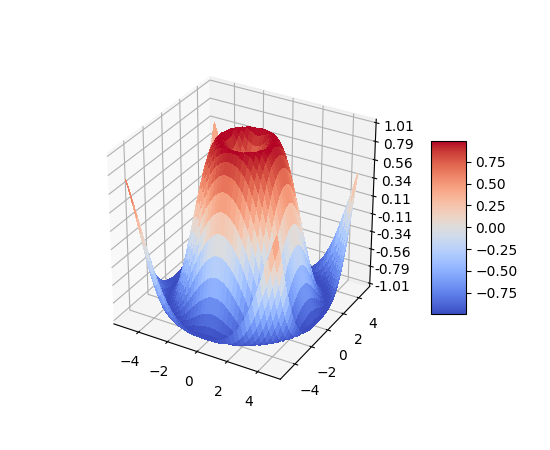
\includegraphics[width=0.25\textwidth]{surface3d_demo4}
    \caption{a nice plot}
    \label{fig:mesh1}
\end{figure}
 
As you can see in the figure \ref{fig:mesh1}, the function grows near 0. Also, in the page \pageref{fig:mesh1} is the same example.

The table \ref{table:1} is an example of referenced \LaTeX elements.
 
%LaTeX Warning: `!h' float specifier changed to `!ht'.
%\begin{table}[h!]
\begin{table}[!ht]
\centering
\begin{tabular}{||c c c c||} 
 \hline
 Col1 & Col2 & Col2 & Col3 \\ [0.5ex] 
 \hline\hline
 1 & 6 & 87837 & 787 \\ 
 2 & 7 & 78 & 5415 \\
 3 & 545 & 778 & 7507 \\
 4 & 545 & 18744 & 7560 \\
 5 & 88 & 788 & 6344 \\ [1ex] 
 \hline
\end{tabular}
\caption{Table to test captions and labels}
\label{table:1}
\end{table}

\section{Aufgabenstellung [todo]}

\section{Motivation [todo]}

\section{Zielsetzung [todo]}

\section{Gliederung [todo]}

\section{???Problemstellung?? [todo]}

In der Zeit vor den Navigationsgeräten wurden auf deutschen Straßen noch regelmäßig faltbare Straßenkarten von den Beifahrern verwendet um den Fahrer den Weg zu weisen. Bevor eine Straßenkarten verwendet werden kann, muss diese Erstellt werden. Dieser Prozess ist unter dem Begriff Kartenerstellung (engl. Mapping) bekannt. Der Detailgrad hängt dabei stark vom Verwendungszweck ab. Der erste Schritt nach dem entfalten der Straßenkarten bestand in der Lokalisierung (engl. Localization), also der Bestimmung der ungefähren Fahrzeugposition und dem Ziel der Reise auf der Straßenkarte. Darauf aufbauend wurde vom Beifahrer dann eine Route zwischen der aktuellen Fahrzeugposition und dem Ziel geplant und während der Fahrt weiter verfolgt, was auch als Pfad-Planung (engl. Path-Planning) bekannt ist.

Genauso wie der menschliche Agent muss auch jeder mobile Roboter für sich diese grundlegende Frage beantworten können. \glqq Wo bin ich?\grqq{}, \glqq Wo bin ich bereits gewesen?\grqq, \glqq Wohin gehe ich?\grqq{} und \glqq Welcher ist der beste Weg dahin?\grqq{}\cite{murphy2000introduction}.

Außerhalb von geschlossenen Räumlichkeiten (engl. Outdoor) erfolgt die Lokalisierung in der Regel mittels GPS, unter der Voraussetzung das eine ungehinderte Verbindung zu den GPS-Satelliten möglich ist. Die Lokalisierung ist in diesem Fall sehr einfach, da die GPS Koordinaten eindeutig sind und das Kartenmaterial bereits im gleichen Koordinatensystem vorliegt.

Innerhalb geschlossener Räumlichkeiten (engl. Indoor), wie in öffentlichen Gebäuden, Logistikhallen oder auch in Bergwerken, ist eine Lokalisierung mittels GPS nicht mehr möglich. Erschwerend kommt dazu, dass es in der Regel zu diesen Räumlichkeiten keine öffentlich verfügbaren Karten gibt oder diese sich wie im letzten Beispiel häufig ändern. Aus diesem Problemfeld haben sich Algorithmen für die Simultane Lokalisierung und Kartenerstellen (engl. Simultaneous Localization and Mapping (SLAM)) entwickelt.

Häufig werden SLAM Algorithmen verwendet um aus Kamerabildern oder \SI{360}{\degree} Abstandsmessungen eine Karte der Umgebung zu erstellen und sich in der gleichen zu lokalisieren. Der Fokus dieser Arbeit liegt jedoch auf den reinen Entfernungsbasieren SLAM (engl. Range Only SLAM (RO--SLAM)) Algorithmen. Hierbei werden nur die Informationen der Eigenbewegung und die Entfernungen zu mehreren, vorher unbekannten, Basisstationen genutzt um sich selbst zu Lokalisieren und eine Karte mit den Positionen der Basisstationen zu erstellen.
	\begin{comment}
------------------------------------------------------------------------------------------
\end{comment}
\chapter{Grundlagen [todo]}


\begin{comment}
------------------------------------------------------------------------------------------
- Der Überblick und Vergleich der verschiedenen Abstandsbestimmungsverfahren erfolgt über eine klassische Literatursuche, siehe \cite{herranz2010studying, zekavat2011handbook}.

	- TDoA, ToF, ToA, AoA, Signal Strength(SS), received signal strength (RSS) , OneWayRanging, TWR
- Wie lange dauert es bis eine Nachricht ausgetauscht worden ist?
	- Beispiel mit einer konkreten Entfernung?
- Wie schnell drifted ein Quarz in einem µc?
	- What is the ppm in the crystal oscillator?
	- https://electronics.stackexchange.com/questions/15851/what-is-the-ppm-in-the-crystal-oscillator
	
\cite{herranz2010studying}
	- Studying of WiFi range-only sensor and its application to localization and mapping systems
\cite{zekavat2011handbook}
	- Handbook of position location: Theory, practice and advances

- \cite{liu2007survey}
	- Survey of wireless indoor positioning techniques and systems (3151)
	- These may be classified based on: 1) the location positioning algorithm, i.e., the method of determining location, making use of various types of measurement of the signal such as Time Of Flight (TOF), angle, and signal strength;
	- Triangulation uses the geometric properties of triangles to estimate the target location. It has two derivations: lateration and angulation.
	- Lateration estimates the position of an object by measuring its distances from multiple reference points. So, it is also called range measurement techniques. Instead of measuring the distance directly using received signal strengths (RSS), time of arrival (TOA) or time difference of arrival (TDOA) is usually measured, and the distance is derived by computing the attenuation of the emitted signal strength or by multiplying the radio signal velocity and the travel time. Roundtrip time of flight (RTOF) or received signal phase method is also used for range estimation in some systems.
	- Angulation locates an object by computing angles relative to multiple reference points. In this survey, we focus on the aforementioned measurements in the shorter range, low-antenna, and indoor environment.
	- TOA: The distance from the mobile target to the measuring unit is directly proportional to the propagation time. In order to enable 2-D positioning, TOA measurements must be made with respect to signals from at least three reference points, as shown in Fig. 1 [4]. For TOA-based systems, the one-way propagation time is measured, and the distance between measuring unit and signal transmitter is calculated. In general, direct TOAresults in two problems. First, all transmitters and receivers in the system have to be precisely synchronized. Second, a timestamp must be labeled in the transmitting signal in order for the measuring unit to discern the distance the signal has traveled.
		- A straightforward approach uses a geometric method to compute the intersection points of the circles of TOA. The position of the target can also be computed by minimizing the sum of squares of a nonlinear cost function, i.e., least-squares algorithm [4], [5].
	- TDOA: The idea of TDOA is to determine the relative position of the mobile transmitter by examining the difference in time at which the signal arrives at multiple measuring units, rather than the absolute arrival time of TOA. For each TDOA measurement, the transmitter must lie on a hyperboloid with a constant range difference between the two measuring units.
		- Wikipedia: Ein Hyperboloid ist im einfachsten Fall eine Fläche, die durch Rotation einer Hyperbel um eine ihrer Achsen entsteht.
		- A 2-D target location can be estimated from the two intersections of two or more TDOA measurements, as shown in Fig. 2. Two hyperbolas are formed from TDOA measurements at three fixed measuring units (A, B, and C) to provide an intersection point, which locates the target P.
	- RSS-Based (or Signal Attenuation-Based) Method: The above two schemes have some drawbacks. For indoor environments, it is difficult to find a LOS channel between the transmitter and the receiver. Radio propagation in such environments would suffer from multipath effect. The time and angle of an arrival signal would be affected by the multipath effect; thus, the accuracy of estimated location could be decreased. An alternative approach is to estimate the distance of the mobile unit from some set of measuring units, using the attenuation of emitted signal strength. Signal attenuation-based methods attempt to calculate the signal path loss due to propagation. Theoretical and empirical models are used to translate the difference between the transmitted signal strength and the received signal strength into a range estimate, as shown in Fig. 3.
		- Due to severe multipath fading and shadowing present in the indoor environment, path-loss models do not always hold.
	- RTOF: This method is to measure the time-of-flight of the signal traveling from the transmitter to the measuring unit and back, called the RTOF (see Fig. 1). For RTOF, a more moderate relative clock synchronization requirement replaces the above synchronization requirement in TOA. Its range measurement mechanism is the same as that of the TOA. The measuring unit is considered as a common radar. A target transponder responds to the interrogating radar signal, and the complete roundtrip propagation time is measured by the measuring units. However, it is still difficult for the measuring unit to know the exact delay/processing time caused by the responder in this case. In long-range or medium-range systems, this delay could be ignored if it is small, compared with the transmission time. However, for short-range systems, it cannot be ignored.
	- Received Signal Phase Method: The received signal phase method uses the carrier phase (or phase difference) to estimate the range. This method is also called phase of arrival (POA) [2].
		- As long as the transmitted signal’s wavelength is longer than the diagonal of the cubic building, i.e., 0 < φi < 2π, we can get the range estimationDi = (cφi)/(2πf).
		- It needs an LOS signal path, otherwise it will cause more errors for the indoor environment.
	- Angulation Techniques (AOA Estimation): In AOA, the location of the desired target can be found by the intersection of several pairs of angle direction lines, each formed by the circular radius from a base station or a beacon station to the mobile target. As shown in Fig. 5, AOA methods may use at least two known reference points (A, B), and twomeasured angles θ1, θ2 to derive the 2-D location of the target P. Estimation of AOA, commonly referred to as direction finding (DF), can be accomplished either with directional antennae or with an array of antennae. The advantages of AOA are that a position estimate may be determined with as few as three measuring units for 3-D positioning or two measuring units for 2-D positioning, and that no time synchronization between measuring units is required. The disadvantages include relatively large and complex hardware requirement(s), and location estimate degradation as the mobile target moves farther from the measuring units. For accurate positioning, the angle measurements need to be accurate, but the high accuracy measurements in wireless networks may be limited by shadowing, by multipath reflections arriving from misleading directions, or by the directivity of the measuring aperture. Some literatures also call AOA as direction of arrival (DOA). For more detailed discussions on AO
	- UWB is based on sending ultrashort pulses (typically <1 ns), with a low duty cycle (typically 1 : 1000). On the spectral domain, the system, thus, uses an UWB (even >500 MHz wide). UWB location has the following advantages [32]. Unlike conventional RFID systems, which operate on single bands of the radio spectrum, UWB transmits a signal over multiple bands of frequencies simultaneously, from 3.1 to 10.6 GHz.
		- At the same time, the signal passes easily through walls, equipment and clothing. However metallic and liquid materials cause UWB signal interference. Use of more UWB readers and strategic placement of UWB readers could overcome this disadvantage. Short-pulse waveforms permit an accurate determination of the precise TOA and, namely, the precise TOF of a burst transmission from a short-pulse transmitter to a corresponding receiver [33], [32]. UWB location exploits the characteristics of time synchronization of UWB communication to achieve very high indoor location accuracy (20 cm). So it is suitable for high-precision real-time 2-D and 3-D location. 3-D location positioning can be performed by using two different measuringmeans: TDOA, which ismeasuring the time difference between a UWB pulse arriving at multiple sensors, and AOA.
		
- \cite{gezici2005localization}
	- Localization via ultra-wideband radios: a look at positioning aspects for future sensor networks (1922)
	- Depending on the positioning technique, the angle of arrival (AOA), the signal strength (SS), or time delay information can be used to determine the location of a node [20]. The AOA technique measures the angles between a given node and a number of reference nodes to estimate the location, while the SS and time-based approaches estimate the distance between nodes by measuring the energy and the travel time of the received signal, respectively.
	- An AOA-based positioning technique involves measuring angles of the target node seen by reference nodes, which is done by means of antenna arrays.
		- The AOA approach is not suited to UWB positioning for the following reasons. First, use of antenna arrays increases the system cost, annulling the main advantage of a UWB radio equipped with low-cost transceivers. More importantly, due to the large bandwidth of a UWB signal, the number of paths may be very large, especially in indoor environments. Therefore, accurate angle estimation becomes very challenging due to scattering from objects in the environment.
	- SS: Relying on a path-loss model, the distance between two nodes can be calculated by measuring the energy of the received signal at one node. This distance-based technique requires at least three reference nodes to determine the 2-D location of a given node, using the well-known triangulation approach depicted in Figure 2 [20]. To determine the distance from SS measurements, the characteristics of the channel must be known. Therefore, SS-based positioning algorithms are very sensitive to the estimation of those parameters.
	- Time-based positioning techniques rely on measurements of travel times of signals between nodes. If two nodes have a common clock, the node receiving the signal can determine the time of arrival (TOA) of the incoming signal that is time-stamped by the reference node.
		- Since the achievable accuracy under ideal conditions is very high, clock synchronization between the nodes becomes an important factor affecting TOA estimation accuracy. Hence, clock jitter must be considered in evaluating the accuracy of a UWB positioning system [25].
		- If there is no synchronization between a given node and the reference nodes, but there is synchronization among the reference nodes, then the time-difference-of-arrival (TDOA) technique can be employed [20]. In this case, the TDOA of two signals traveling between the given node and two reference nodes is estimated, which determines the location of the node on a hyperbola, with foci at the two reference nodes. Again a third reference node is needed for localization. In the absence of a common clock between the nodes, round-trip time between two transceiver nodes can be measured to estimate the distance between two nodes [26], [27].
- \cite{decawave2014rtls}
	- Real time location systems - An Introduction
	- There are a number of different methods of implementing RTLS using wireless schemes but they effectively devolve into two basic types of scheme:
		 Those based on radio signal strength – commonly referred to as Received Signal Strength Indication or RSSI schemes.
		 Those based on the measurement of Time – where the time it takes the radio signal to travel between transmitter and receiver is measured using one or more of a variety of different techniques and then knowing the speed of light the distance can be calculated.
	- Signal Strength Based Schemes
		- These schemes involve measuring the signal strength of the arriving radio signal at the receiver. Knowing the power at which the signal was transmitted from the transmitter, the propagation characteristics of that particular radio signal in air and with some a priori knowledge of the environment it is possible to calculate approximately where the transmission originated based on how attenuated it is at the receiver.
		- We will not consider these schemes any further here since time-based schemes using Ultra Wideband can achieve a far more accurate result.
	- 3.2 Time Based Schemes
		- These are all referred to as time-based schemes because they are all based on the accurate measurement of the propagation time of a radio signal from one location to another or the difference in arrival time of a radio signal at different locations.
		- Time of Flight: All time of flight based systems work on the basis of determining the time it takes for a radio signal to propagate from a transmitter to a receiver. Once this time is known accurately then the distance between the transmitter and the receiver can be determined since the speed of propagation of radio waves in air is known.
			- Calculating the point of intersection between these three circles (tri-lateration) gives the position of the tag B. If the absolute location of the anchors is know in 2D or 3D space then the absolute location of the tagged object is also known.
		- Time Synchronized Transmitter and Receiver: In this case the tagged object (transmitter) and the Anchor (receiver) are synchronized in time. In this scheme the tag (B) broadcasts a message to all of the anchors simultaneously (P1, P2 & P3) at a known time (or with the transmit time embedded in the message). Each anchor receives the message and because it knows when the message was transmitted, when it was received and because all times are relative to a common time-base it can calculate the time of flight and therefore the distance.
			- The drawback with this system is that it requires all elements of the system to be time synchronized. This is difficult enough in the case of anchors, as we’ll see later, but is extremely difficult to do in the case of mobile tags. For that reason, this system is seldom used.
		- Unsynchronized Transmitter and Receiver: In this case the tagged object communicates with each of the fixed anchors in what’s called a two-way ranging exchange. The tag and each anchor exchange timing information so that the anchor can calculate the time-of-flight of the signal from the tag to the anchor without the necessity for tag and anchor to be synchronized in time. Once each anchor has this information, a location engine can calculate the position of the tagged object.
			- This requires that the tag be capable of receiving as well as transmitting which means that this method generally consumes more power than the Time Difference of Arrival solution we’ll see in the next section.
				 The anchor transmits a message to the tag and records the time the message left its antenna (let’s call it t1).
				 The tag receives the message and sends back a reply.
				 The anchor records the time it receives the reply (let’s call it t2)
				 The anchor then calculates the time difference Tr = t2 – t1
				 The anchor then calculates the distance using the formula d = cTr/2, where c is the speed of light.
			- This is what’s known as Two Way Ranging.
		- Time Difference of Arrival: In this scheme three or more readers are positioned in known locations around the area in which tagged items are to be located. Each of these readers is time synchronized to the others.
			- As shown in Figure 6 a tagged object (B) transmits a message that is received by all the readers (P1, P2 and P3 in the diagram shown here). Because radio waves travel at a constant speed, depending on the position of the tagged object, the message will arrive at some of the anchors before others. The time of arrival of the message at each reader is noted by the reader.
			- Since all three readers are time-synchronized, the difference in the time of arrival at each of the three readers gives information about the location of the tag B
			- Using a mathematical technique known as multi-lateration it is then possible to derive the position of the tag
			- Since the tag only transmits and does not receive, this is also known as One Way ranging but is not possible with only one reader since it relies on the difference in the arrival times at several readers to calculate the location
			- The most important system issue here is that the anchors must be synchronized in time. Any error in the synchronization of time in the anchors translates directly to an error in the reported location. When you think that 1ns = approx 30cm then it’s clear that synchronization needs to be to the sub-nanosecond level. Traditionally this has been achieved by wiring clock signals from a central clock distribution point to all the anchors and compensating for delays in the distribution cabling. As you can imagine this makes system installation very expensive. DecaWave have developed a wireless synchronization scheme that allows the anchors to be synchronized to the required level of accuracy without extra cables.
		- Angle of Arrival (AoA): Angle of Arrival involves determining the angle at which the radio signal from the tag arrives at the anchor relative to a predefined direction.
			- This scheme is generally implemented using an array of antennas in the anchor.
			- If the tag is at some angle to the array then the incident signal will reach one antenna in the array first followed by the next and so on.
			- Assuming these arrival times can be measured accurately then a measure of the angle of arrival can be made.
			- Angle of Arrival schemes don’t deal particularly well with multipath propagation between the transmitter and the receiver antenna array and so are best suited to Line of Sight scenarios.
			
- \cite{decawave2015twr}
	- The implementation of two-way ranging with the DW1000
	- In this application note two-way ranging (TWR) scheme as used by Decawave’s example application (DecaRanging) is described. TWR is a basic concept to calculate the distance between two objects by determining the time of flight (TOF) of signals travelling between them.
	- The DW1000 uses mathematical and electronic techniques to implement a very precise clock. By recording the state of this clock when certain events occur during DW1000 transmission and reception of the radio wave signals, the DW1000 has the ability to ‘timestamp’ those events.
	- DW1000 based TWR
		- The initiator transmits a radio message to the responder and records its time of transmission (transmit timestamp) t1. The responder receives the message and transmits a response (a radio message) back to the initiator after a particular delay treply. The initiator then receives this response and records a receive timestamp t2.
		- If we assume the speed of radio waves through air is the same as the speed of light c, then the distance between the initiator and responder can be calculated by,
		- there are a number of sources of error due to clock drift and frequency drift [4]. Asymmetric double sided TWR method is used in Decawave’s implementation. It reduces the error due to clock and frequency drift.
	- Discovery and Ranging phase message exchanges
- \cite{decawave2016dw1kusermanual}
	- Single-sided two-way ranging (SS-TWR)
	- Double-sided two-way ranging (DS-TWR)
		- The four messages of DS-TWR, shown in Figure 37, can be reduced to three messages by using the reply of the first round-trip measurement as the initiator of the second round-trip measurement.
	- Error
		- Where the clock in device A runs at ka times the desired frequency and the clock in device B runs at kb times the desired frequency and both ka & kb are close to 1.
		- To give some idea of the size of this error, if devices A and B have clocks where each are 20 ppm away (the worst case specification) from the nominal clock in directions which make their combined error additive and equal to 40 ppm, then ka and kb might both be 0.99998 or 1.00002.
		- Even with a relatively large UWB operating range of say 100 m, the TOF is just 333 ns, so the error is 20 × 10-6 × 333 × 10-9 seconds, which is 6.7 × 10-12 seconds or 6.7 picoseconds which is approximately 2.2 mm.

	
\end{comment}
\section{Verfahren für die Reichweiten-Bestimmung [todo]}

% Wikipedia: Lateration (lat. lateral = seitlich) oder Trilateration ist ein Messverfahren zur Positionsbestimmung eines Punktes. Während die Triangulation auf der Vermessung dreier Winkel basiert, beruht die Trilateration auf Entfernungs- bzw. Abstandsmessungen zu drei Punkten. https://de.wikipedia.org/wiki/Lateration



\subsection{Two Way Ranging}
\subsection{Symmetric Double-Sided Two-Way Ranging (SDS-TWR)}








\begin{comment}
------------------------------------------------------------------------------------------
- Theorie: Wahrscheinlichkeitsverfahren
	- Positionsschätzer in Form einer Wahrscheinlichkeitsverteilung über den Zustandraum.
	- Kalman fitering
		- Multivariate Gaussian distribution (Mehrdimensionale Normalverteilung)
		- \url{https://de.wikipedia.org/wiki/Mehrdimensionale_Normalverteilung}
		- Kompakte Beschreibung der Normalverteilung über den Erwartungswert $\mu$ und die Kovarianzmatrix $\Sigma$ ($\mu$ und $\sigma^2$)
		- \url{https://matheguru.com/stochastik/normalverteilung.html}
	- Markov methods
		- Probability Grid
		- Robot--Position ist diskretisiert
		- Nutzen von Bayes Rule um Grids zu kombinieren/neuerzeugen
	- Monte Carlo Lokalisierung
		- Multimodal Distribution for position estimation
		- Important Sampling
\end{comment}
\section{Wahrscheinlichkeitstheorie [todo]}


\begin{comment}
------------------------------------------------------------------------------------------
- Theorie: Lokalisierungsprobleme
	- Statische Lokalisierung
		- Akkurate Schätzung seiner globalen Position anhand der Sensordaten
		- Annahme: Umgebungskarte der Landmarken ist vorhanden
	- Position Tracking/Positionsverfolgung
		- Initiale Position ist gegeben
		- Verfogenden der Roboterposition
		- Annahme: Umgebungskarte der Landmarken ist vorhanden
	- SLAM
		- Verwenden der Sensordaten um sich zu Lokalisierung...
		- und eine Karte der Landmarken zu erzeugen.
		- Bisher Winkel und Entferung zu einer Landmarke gegeben
			- Computer Vision, Structure from Motion
		- Hier nur die Entfernung
\end{comment}
\section{Bayes/Kalman/Partikel Filter [todo]}


\begin{comment}
------------------------------------------------------------------------------------------
- \cite{kalman1960new}
- \cite{kurth2003experimental}
	- Originally introduced in 1960, the Kalman lter assumes a multivariate Gaussian distribution [6]. The Kalman lter has the advantage that the representation of the distribution is compact; a Gaussian distribution can be represented by a mean and a covariance matrix. The robot's pose estimation is maintained as a Gaussian distribution and sensor data from dead reckoning and landmark observations is fused to obtain a new position distribution.
	- Our results with Kalman ltering require an under-standing of the characteristics of the noise present in ranges reported by the radio tags. We gain this by look-ing at the probability distribution functions for each tag measurement.
	- We obtain the PDFs as follows: for every reported measurement, we nd the true range to the robot when that distance was reported. We do this by comparing the known location of the reporting tag to the times-tamped true location of the robot when the report was received.
	- the covariance matrix, which describes the uncertainty and correlation of the terms in the state estimate.
	- However, when the same initial noisy tag locations are used with Test 2, our SLAM technique fails to converge. Since the Kalman lter uses a linearization of the nonlinear range measurements, if the linearized estimate is too far away from the truth, the lter may be unable to recover and will diverge.
	-

\end{comment}
\section{Kalman Filter [todo]}




\begin{comment}
------------------------------------------------------------------------------------------
- \cite{kurth2003experimental}
	- Recent extensions of Kalman ltering allow for non-Gaussian, multimodal probability distributions through multiple hypothesis tracking. The result is a more versatile estimation technique that still preserves many of the computational advantages of the Kalman filter.
\end{comment}
\subsection{Extended Kalman Filter [todo]}

% Linearisierung


\begin{comment}
------------------------------------------------------------------------------------------
\end{comment}
\section{Partikel Filter [todo]}

\begin{comment}
------------------------------------------------------------------------------------------
- \cite{kurth2003experimental}
	- Monte Carlo localization, or particle ltering, provides a method of representing multimodal distri-butions for position estimation [4, 12], with the ad-vantage that the computational requirements can be scaled. The main advantage of these methods is their ability to recover robustly from a poor initial condition.
\end{comment}
\subsection{Monte Carlo [todo]}

\cite{fox1999monte}, 

\begin{comment}
------------------------------------------------------------------------------------------
Rao-Blackwellized Particle Filtering
https://people.eecs.berkeley.edu/~pabbeel/cs287-fa12/slides/RBPF.pdf
\end{comment}
\subsection{Rao-Blackwellized [todo]}


\begin{comment}
------------------------------------------------------------------------------------------
- \cite{kurth2003experimental}
	- We are currently developing a batch localization method, which considers all the data collected by the robot and nds the best path estimate given all the data. Although time consuming computationally, this will produce the theoretically optimal result obtainable from the collected data; we can then evaluate the results of our online localization method by comparing to this optimal solution.
\end{comment}
\section{Batch optimization [todo,optional]}


\begin{comment}
------------------------------------------------------------------------------------------
- \cite{kurth2003experimental}
	- Additionally, we will extend the batch method to produce a variable dimension lter, as used by Deans for the case of bearing-only sensors [3], which would consider some window of previous robot states and optimize the position estimates based on the data in that window.
\end{comment}
\section{Variable Dimension Filter [todo,optional]}


\begin{comment}
------------------------------------------------------------------------------------------
Embodied Localisation and Mapping
http://elib.suub.uni-bremen.de/edocs/00103537-1.pdf

- \cite{sarkka2013bayesian}
	- Bayesian filtering and smoothing
- \cite{kurth2003experimental}
	- The Kalman lter approach described in Section 5 can be reformulated for the SLAM problem. To perform SLAM, we include position estimates for each tag in the state, producing a state vector of the form: q(k) = [xk; yk; k; xb1; yb1 ; :::; xbn; ybn]T , where n is the number of beacons.
\end{comment}
\section{SLAM [todo]}

% Zuerst wird die Position geschätzt und danach die Positionen der Landmarken.


\begin{comment}
------------------------------------------------------------------------------------------
\end{comment}
\section{ROS [todo]}
	%
% Forschungsstand:
%
% - Welche wissenschaftlichen Erkenntnisse liegen zu dem Thema bereits vor?
% - Grundsätzlich gibt es zwei Möglichkeiten, einen Forschungsstand zu schreiben: Entweder ordnen Sie Ihren Literaturüberblick nach Themenkomplexen oder Sie geben einen rein chronologischen Überblick über die wichtigsten Publikationen.
% - Auf keinen Fall sollten Sie den Forschungsstand zu voll packen. Es geht nicht darum, dem Leser zu zeigen, was Sie alles studiert haben (wie fleißig Sie waren), sondern um einen kompakten Überblick über die wichtigste Literatur.
% - Wichtig: Listen Sie die Literatur nicht nur auf, sondern erklären Sie, welchen Beitrag die jeweilige Publikation zum Erkenntnisgewinn geleistet hat. Also, zum Beispiel: Was hat der Autor als Erster erkannt oder hinterfragt? Es muss ja einen Grund geben, weshalb Sie die betreffende Publikation unter die Meilensteine reihen – und den sollten Sie dem Leser deutlich machen.
%
% Ferrein:
% - 4-5 Seiten in der Bachelorarbeit (deutlich umfangreicher als im Exposé)
% - Was unterscheidet meinen Ansatz von den anderen verhandenen Ansätzen?
%

\begin{comment}
------------------------------------------------------------------------------------------
- Informationen aus dem Expose
	- Einen guten Überblick über die Eigenschaften der Drahtlosen-Protokolle (engl. Wireless Protocols) Bluetooth, UWB, ZigBee und WiFi liefert die Arbeit \cite{lee2007comparative} von \citeauthor{lee2007comparative}.
	- In \cite{smith1987closed} wird das grundlegende Prinzip erklärt um aus mehreren bekannten Sensoren die Position eines beweglichen Empfängers zu berechnen.
	- Der theoretische Hintergrund des SLAM--Verfahrens wird in \cite{dissanayake2001solution} vorgestellt. Zusätzlich wird bewiesen das die Unsicherheit bei der Kartenerstellung und Lokalisierung eine untere Schranke erreicht.
	- \citeauthor{kantor2002preliminary} stellen in Ihrer Arbeit \cite{kantor2002preliminary} ein Lokalisierungsverfahren vor, welches die Roboterposition anhand von Entfernungsmessungen zu vorher bekannten Landmarken bestimmen kann. Im letzten Abschnitt wird SLAM--Verfahren vorgestellt, welches über einen Kalman--Filter die Unsicherheit der Landmarkenposition modellieren kann.
	- Die Autoren \citeauthor{blanco2008pure} gehen in ihren Arbeiten \cite{blanco2008pure, blanco2008efficient} einen Schritt weiter und bestimmen die unbekannte Roboterposition sowie die unbekannten Landmarkenpositionen. Hierzu nutzen Sie im ersten Schritt einen Partikelfilter (engl. Particle Filter) bis die Schätzung eine ausreichende Genauigkeit erreicht hat um dann im zweiten Schritt über einen Kalman--Filter ein Positionsverfolgung (engl. Position Tracking) durchzuführen.
	- Die Arbeit \cite{ledergerber2015robot} von \citeauthor{ledergerber2015robot} gehen auf die Roboterlokalisierung unter Verwendung einer One-Way Ultra-Wideband Kommunikation ein. Dieses hat den Vorteil, das mit sehr wenigen Landmarken eine große Anzahl von Roboter lokalisiert werden kann.
	
	- The Cartesian EKF described above operates in the Cartesian space, we formulate our problem in polar coordinates.
	
	- The use of this parameterization derives motivation from the polar coordinate system, where annuli, crescents and other ringlike shapes can be easily modeled. This parameterization is called Relative Over Parameterized (ROP) because it over parameterizes the state relative to an origin.

	- EKF -> Polar EKF -> Multi-Hypothesis Filter
	
	- Partikel Filter
\end{comment}


\begin{comment}
------------------------------------------------------------------------------------------
\end{comment}
\chapter{Stand der Forschung und Technik [rework]}

In diesem Kapitel wird ein chronologischer Überblick über die wichtigsten Publikationen zum Thema \Gls{roslam} geliefert. Jeder Autor verwendet eine etwas andere Terminologie, auch wenn es sich im Kern um die gleiche Sache handelt. Daher werden in diesem Kapitel die Begriffe Anker, Tag und Beacon synonym verwendet.


\begin{comment}
------------------------------------------------------------------------------------------
- \cite{kantor2002preliminary}
- Preliminary results in range-only localization and mapping (189)
- Section 2
	- Statische Lokalisierung
		- Vorherige Sensorinformationen und Positionsschätzung werden nicht genutzt.
		- Annahme: Position der Beacons ist bekannt und fix.
	- Markovian probability grids
	- Mit fehlerfreien Messungen ist die Positionsbestimmung trivial
	- Entfernungsmessung mit einem erwarteten Fehler von 6 feet, also 1,82 meter. (1Fuß==30cm)
	- 1. Characterizing Range Measurements
		- Erstellen einer Verteilungsfunktion für die Entfernungsmessung
		- experimentel bestimmt
		- Diskrete Messungen in einem Set {0,6,12,...,50}
	- 2. Creating Probability Grids
		- Für jede Zelle des Grid wird die Wahrscheinlichkeit mittels der PDF berechnet.
	- 3. Combine Probability Grids
		- Multiply in a pointwise manner
		- scale the result so that the sum over the squares is one.
		- Aus den kombinierten Ergebnisgrid kann die schätzte Position mittels der gewichteten Durchschnitt der Gridzellen berechnet werden.
		- Covariance Matrix lässt sich auch bestimmen
	- Durchschnittlich geschätzer Fehler lag ab 1,62 feet bei einem geschätzen Entfernungsmess Fehler von 5.82 bis 7.18 feet.
- Section 3
	- Beacon positionen sind bekannt
	- Vorherige Positionsschätzung und Odometry daten werden verwendet.
	- Positionsverfolgung mittels Kalman und Monte Carlo
	- Kalman
		- Initiale Positionsschätzung wie in Section 2, jedoch mit drei Beacons.
		- Approximieren eines ringförmigen Gauß-Verteilung um die geschätzte Position.
		- Füttern eines entsprechenden EKF mit den Parametern
	- Monte Carlo
		- Verwendet die pdf aus Section 2 um die Partikels zu gewichten.
	- Durchschnittliche Geschätzter Fehler
		- EKT: 0,73 feet
		- MC: 0,93 feet
- Section 4
	- Lokalisieren in einer Umgebung mit unsicheren beacon positionen
		- Approximately known, good but not perfect
		- crude measurement or estimate location on blueprint
	- SLAM mit EKF
		- State ist die Robot-- und Beacon--Position
		- Error: init 5.13 feet, end 0.77 feet
\end{comment}
\section{Preliminary results in range-only localization and mapping}

In \citetitle{kantor2002preliminary}\cite{kantor2002preliminary} verwendet der Author \Glspl{beacon} die eine Entfernungsschätzung mit einem mittleren Fehler von \SI{1.82}{\metre} (6 Fuß) liefern. Um das Problem der Datenzuordnung zu trivialisieren, liefert jeder \Gls{beacon} zusätzlich zur Messung eine eindeutigen Identifikationsnummer mit. Nur mit diesen Daten werden die Probleme der Roboter Lokalisierung, Positionsverfolgung und \Gls{slam} behandelt. Das algorithmische Fundament wird dabei durch den \Gls{ekf} und \Gls{mc} Partikelfilter gebildet.

Im ersten Abschnitt wird die statische Lokalisierung thematisiert, die für eine Positionsschätzung auf vorherige Sensorinformationen und Positionsschätzungen verzichtet. Bei einer fehlerfreien Entfernungsmessungen ist die Positionsbestimmung ein mathematisch triviales Problem. Da die Messungenauigkeit mit \SI{1.82}{\metre} jedoch sehr hoch ist, werden Methoden der Wahrscheinlichkeitstheorie verwendet. Im ersten Schritt wird die Verteilungsfunktion experimentell für einige diskreten Abstände bestimmt. Unter zuhilfenahme der erstellten Verteilungsfunktion wird für jeden \Gls{beacon} und für jede Zelle des \Gls{propgrid} die Wahrscheinlichkeit berechnet, siehe \figurename~\ref{fig:kantor2002preliminary_figure1b} links. Im letzten Schritt werden die einzelnen \Gls{propgrid} miteinandern multipliziert und im Abschluss skaliert damit die Summe über alle Zellen gleich eins ist, siehe \figurename~\ref{fig:kantor2002preliminary_figure1c} rechts. Aus dem gewichteten Durchschnitt der Zellen lässt sich die Position schätzen, siehe \figurename~\ref{fig:kantor2002preliminary_figure1c}. Der durchschnittliche Schätzungsfehler beträgt \SI{0.49}{\metre} bei einem erwarteten Fehler von \SIrange{1,77}{2,18}{\metre} bei der Entfernungsmessung.

\begin{figure}[htbp]
  \begin{minipage}[t]{0.45\linewidth}
    \centering
    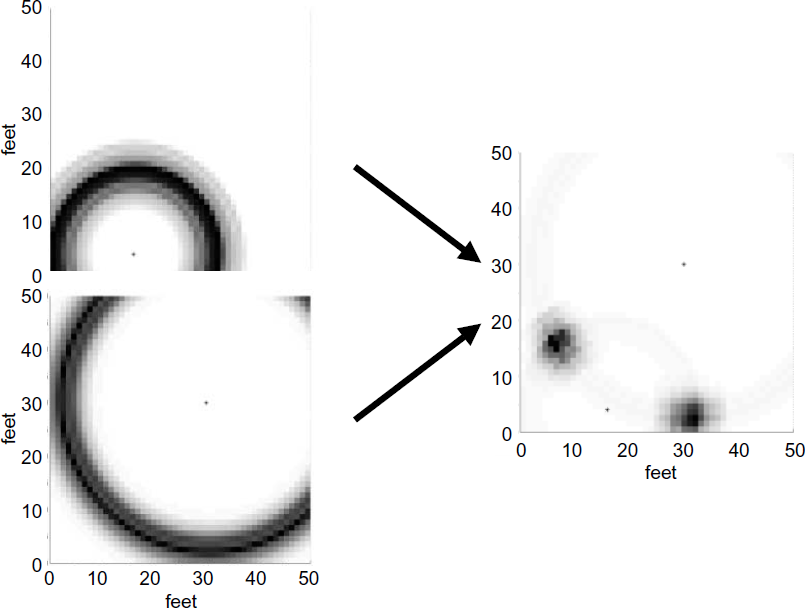
\includegraphics[width=\linewidth]{kantor2002preliminary_figure1b}
    \caption{Links: \Gls{propgrid} pro \Gls{beacon}. Rechts: Kombination zweier \Glspl{propgrid}.}
    \label{fig:kantor2002preliminary_figure1b}
  \end{minipage}
  \hfill
  \begin{minipage}[t]{0.45\linewidth}
    \centering
    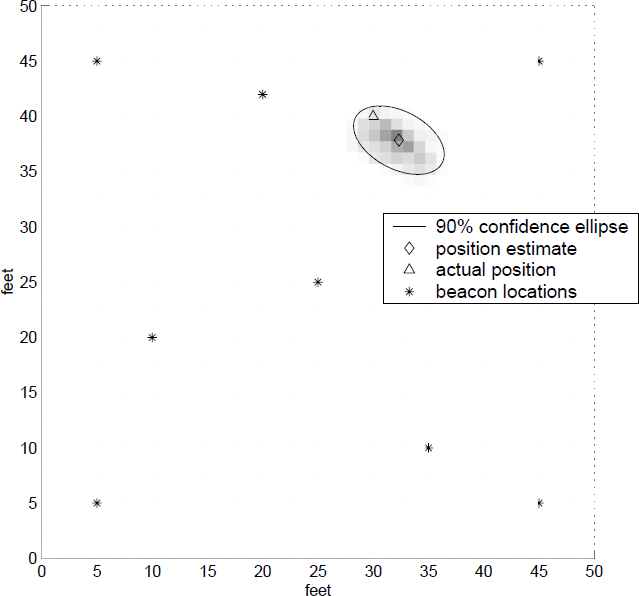
\includegraphics[width=\linewidth]{kantor2002preliminary_figure1c}
    \caption{Kombiniertes \Gls{propgrid} aller \Glspl{beacon}.}
    \label{fig:kantor2002preliminary_figure1c}
  \end{minipage}
	\source{\cite{kantor2002preliminary}}
\end{figure}

Im nächsten Abschnitt wird die Positionsverfolgung mittels eines \Gls{ekf} bzw. \Gls{mc} Partikelfilter behandelt. Hier für werden die Odometriedaten und die vorhergie Positionsschätzung verwendet. Für eine initiale Positionsschätzung wird das Verfahren aus dem vorherigen Abschnitt verwendet. Aus der Entfernungsschätzung eines \Glspl{beacon} ergibt sich eine ringförmige Verteilungsfunktion, die mit einer unimodalen Verteilung nicht modelliert werden kann. Als Annäherung wird eine Normalverteilung verwendet, die in tangentialer Richtung gestreckt und in radialer Richtung gestaucht ist. Als Mittelwert wird die vorherige Positionsschätzung verwendet, siehe \figurename~\ref{fig:kantor2002preliminary_figure2}. Um die Partikel im \Gls{mc} Partikelfilter zu gewichten ist die ringförmige Verteilung vollkommen ausreichend. Der durchschnittliche Schätzungsfehler beträgt beim \Gls{ekf} \SI{0.22}{\metre} und \SI{0.28}{\metre} beim \Gls{mc} Partikelfilter.

\begin{figure}[htbp]
	\centering
	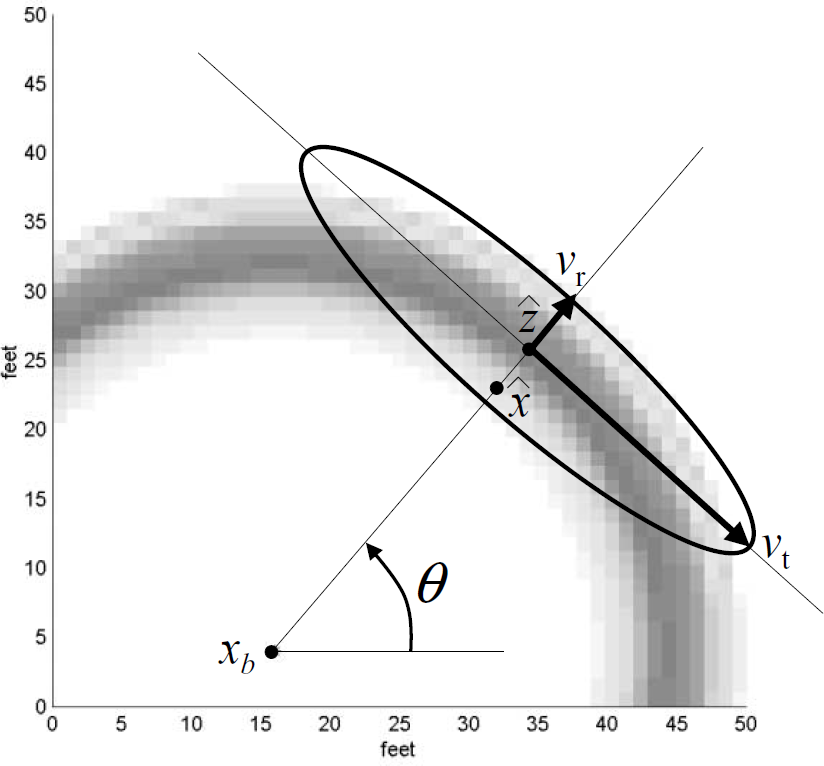
\includegraphics[width=0.5\linewidth]{kantor2002preliminary_figure2}
	\caption{Annäherung einer ringförmigen Verteilung an eine Normalverteilung.}
	\label{fig:kantor2002preliminary_figure2}
	\source{\cite{kantor2002preliminary}}
\end{figure}

Der letzte Abschnitt wird ein \Gls{slam}--Verfahren mittels einem \Gls{ekf} behandelt. Die initiale Roboter-- und \Gls{beacon}--Position muss nicht genau jedoch ungefähr bekannt sein. Der Zustandsvektor des \Gls{ekf} beinhaltet die Roboter-- und alle \Gls{beacon}--Positionen. Der durchschnittliche Fehler in der initalen Schätzung beträgt \SI{1.56}{\metre} und verbessert sich zum Schluss hin auf \SI{0.23}{\metre}.


\begin{comment}
------------------------------------------------------------------------------------------
- \cite{kurth2003experimental}
	- Experimental results in range-only localization with radio (82)
\end{comment}
%\section{Experimental results in range-only localization with radio [todo]}


\begin{comment}
------------------------------------------------------------------------------------------
- \cite{olson2004robust}
	- Robust range-only beacon localization (264)
	- Wie funktioniert die Exploration Strategy?
		- Die Ungünstigeste strategy ist das geradeausfahren mit einem beacon links und rechts.
		- Das Gradientenfeld der abstanddifferenz zwischen den beiden beacons führt einen auf den optimalen weg um die Abstandsdifferenz zu maximieren. (Aktive Exploration)
\end{comment}
\section{Robust range-only beacon localization}

In \citetitle{olson2004robust}\cite{olson2004robust} werden autonome Unterwasserfahrzeuge (engl. \gls{auv}) verwendet um den Ozeanen der Welt die letzten Geheimnisse zu entlocken. Hierfür ist eine genaue Lokalisierung der \gls{auv} notwendig. Dies wird über die Messung der Signallaufzeit zwischen dem \gls{auv} und mehreren stationären akustischen Transponder--\Gls{beacon} erreicht. Vor der eigentlichen Messung müssen jedoch die \Glspl{beacon} im Messbereich verteilt werden, deren Position genau bestimmt werden und zusätzlich dafür gesorgt werden, dass die \Glspl{beacon} ihre Position nicht ändern. Dadurch handelt es sich um ein sehr kostspieliges Prozedere und soll in dem vorgestellt Verfahren dahingehend optimierte werden, dass die \Gls{beacon}--Position vorher nicht bekannt sein muss. Dadurch ist eine autonome Verteilung der \Glspl{beacon} möglich und zusätzlich kann auch detektiert werden ob ein \Gls{beacon} seine Position verändert hat.

% TODO: Spectral Graph Partitioning Übersetzung? 
Bevor jedoch die Laufzeitmessungen verwendet werden können, müssen diese um \Gls{outlier} (dt. Ausreißer) bereinigt werden. Diese entstehen z.B. durch unterschiedliche Ausbreitungsgeschwindigkeiten der Schallwellen im Wasser, durch Reflektionen am Meeresgrund (engl. \Gls{multipath}) oder durch Interferenzen der Nutzlast (engl. \Gls{payload}) mit den Sensoren. Die Bereinigung der Messdaten erfolgt hierbei über das \textit{Spectral Graph Partitioning} Verfahren. Hierbei wird jede Messung als Kreis dargestellt. Überschneiden sich zwei Kreise gelten diese beiden Messungen als konsistent. Jede der Messungen wird in einem Graphen zu einem Vertex und jede konsistente Messung zu einer Kante. Bei dem fertigen Graphen ist nun zu beobachten, dass \Gls{outlier} weniger stark untereinander verbunden sind als \Gls{inlier}. Diese durchschnittliche Konnektivität der \Gls{inlier} wir als Metrik für den Partitionierungsalogorithmus verwendet um die Messdaten zu filtern.

Nach dem die Messwerte pro \Gls{beacon} gefiltert worden sind, werden zwei Messwerte von zwei verschiedenen \Glspl{beacon} wieder mit einandern überschnitten. Hieraus entstehen zwei mögliche Positionen des \gls{auv}. In einem Grid erhöhen diese beiden Positionen dann den Ihnen zugeordneten Zähler. Dieser Vorgang wird für weiter Messwerte wiederholt. Durch das daraus resultierende Voting--System entstehen zwei Gipfel (engl. Peak) die die mögliche Position des \gls{auv} approximieren. Ist der Höhenunterschied zwischen den Gipfeln ausreichend groß, wird die \gls{auv}--Position mit dem höchsten Gipfel an einen EKF--SLAM übergeben.


\begin{comment}
------------------------------------------------------------------------------------------
-\cite{smith2004tracking}
	- Tracking moving devices with the cricket location system (547)
\end{comment}
%\section{Tracking moving devices with the cricket location system [todo]}


\begin{comment}
------------------------------------------------------------------------------------------
\end{comment}
\section{A pure probabilistic approach to range-only SLAM}\label{sec:blanco2008pure}

Alle zuvor vorgestellten Verfahren hatten den Nachteil, dass sie probabilistische und nicht probabilistische Verfahren gemeinsam verwendeten um eine initiale Schätzung der \textit{Beacon}--Positionen zu erlangen. In dieser Initialisierungsphase waren alle Positionsinformationen für die Positionsschätzung des Roboters verloren. In der Arbeit \citetitle{blanco2008pure} \cite{blanco2008pure} wird zu jedem Zeitpunkt die beste \textit{Beacon}--Schätzung genutzt um die Roboterposition zu verbessern. Um das zu bewerkstelligen, wird ein rein probabilistisches Verfahren genutzt.

Verwendung findet hierbei der \Gls{rbpf}, der die Berechnung des Roboterpfades von der Karte mit den Landmarken entkoppelt \cite{murphy2001rao, montemerlo2002fastslam}. Jeder Partikel des \Gls{rbpf} beschreibt dabei pro \textit{Beacon} die Verteilung die am besten zu seiner Positionsschätzung passt. Die Verteilung wird dabei zuerst von einem Hilfspartikelfilter (engl. Auxiliary Particle Filter) modelliert. Seine Partikel besitzen dabei eine ringförmige Verteilung mit dem Abstand des \textit{Beacon}, siehe \figurename~\ref{fig:blanco2008pure_fig3e}. Partikel mit einer geringen Wahrscheinlichkeit werden über eine Gewichtung aussortiert, siehe \figurename~\ref{fig:blanco2008pure_fig3f}. Sobald der Hilfspartikelfilter gegen eine bestimmte \textit{Beacon}--Position konvergiert ist, wird dieser in einen Normalverteilung umgewandelt und über einen \Gls{ekf} modelliert, siehe \figurename~\ref{fig:blanco2008pure_fig3g}.

\begin{figure}
	\begin{subfigure}[t]{0.3\linewidth}
		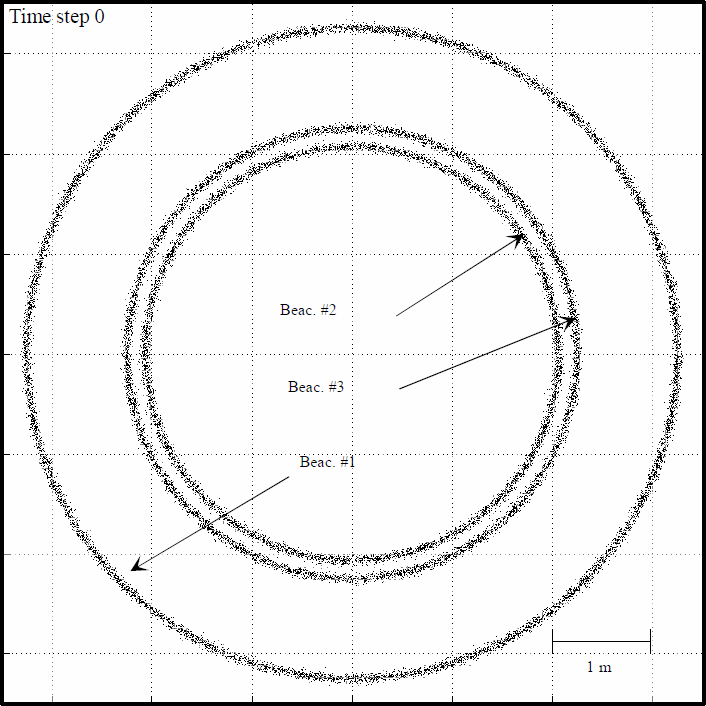
\includegraphics[width=\linewidth]{blanco2008pure_fig3e}
		\caption{}
		\label{fig:blanco2008pure_fig3e}
	\end{subfigure}
	\hfill
	\begin{subfigure}[t]{0.3\linewidth}
		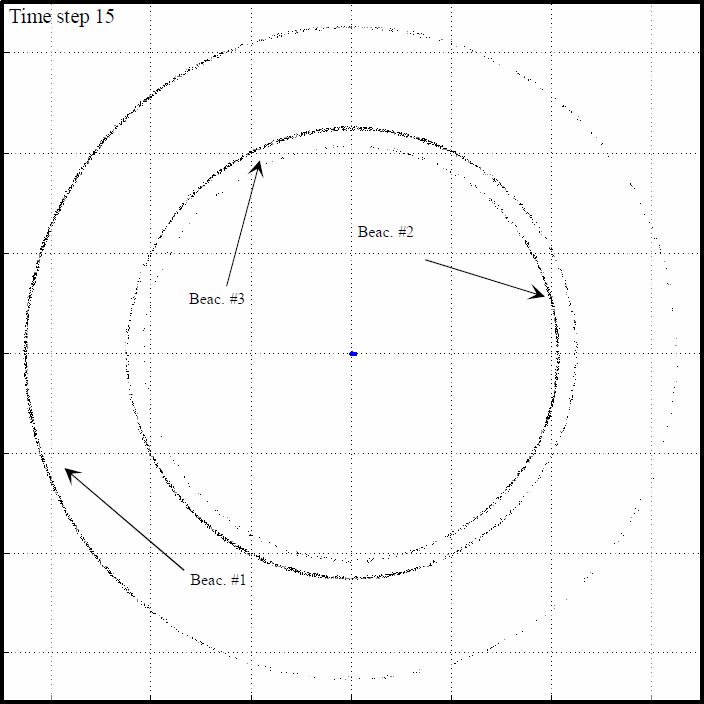
\includegraphics[width=\linewidth]{blanco2008pure_fig3f}
		\caption{}
		\label{fig:blanco2008pure_fig3f}
	\end{subfigure}
	\hfill
	\begin{subfigure}[t]{0.3\linewidth}
		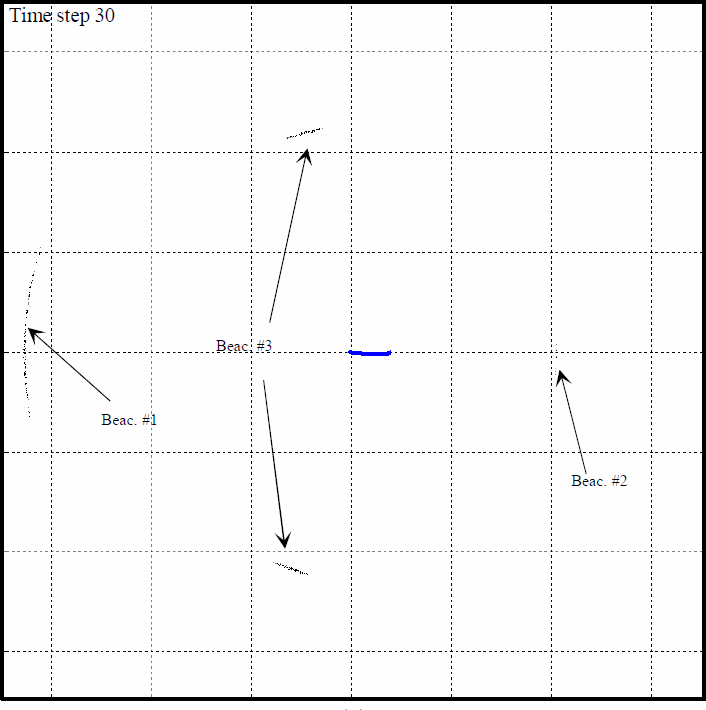
\includegraphics[width=\linewidth]{blanco2008pure_fig3g}
		\caption{}
		\label{fig:blanco2008pure_fig3g}
	\end{subfigure}
	\caption{Entwicklung eines Hilfspartikelfilters zu einem \Gls{ekf}.}
	\label{fig:blanco2008pure_fig3}
	\source{\cite{blanco2008pure}}
\end{figure}


\begin{comment}
------------------------------------------------------------------------------------------
- \cite{blanco2008efficient}
	- Efficient probabilistic range-only SLAM (71)
\end{comment}
\section{Efficient probabilistic range-only SLAM}\label{sec:blanco2008efficient}

Aufbauend auf der vorherigen Arbeit im Abschnitt~\ref{sec:blanco2008pure} wird in \citetitle{blanco2008efficient} \cite{blanco2008efficient} nicht mehr ein Hilfspartikelfilter verwendet, der ab einer gewissen Sicherheit in einen \Gls{ekf} umgewandelt wird. Stattdessen wird die ringförmiger Verteilung über radial angeordnete Normalverteilungen angenähert deren Nachbarschaftsabstand über den Parameter \textit{K} bestimmt werden kann, siehe \figurename~\ref{fig:blanco2008efficient_fig17a}~--~\ref{fig:blanco2008efficient_fig17b}. Die Gesamtverteilung ergibt sich dabei über eine gewichtete Summe der Normalverteilungen (engl. Sum of Gaussians). Über die Gewichte lässt sich dabei steuern, ob eine der Normalverteilungen in dem Ring für die \textit{Beacon}--Position noch relevant ist oder entfernt werden kann, siehe \figurename~\ref{fig:blanco2008efficient_fig10a}~--~\ref{fig:blanco2008efficient_fig10b}.

Sowohl das Verfahren aus dem Abschnitt~\ref{sec:blanco2008pure} als auch dieses sind in dem \Gls{mrpt}--Framework vorhanden und werden im Kapitel~\ref{ch:ro_slam} verwendet.

\begin{figure}[!ht]
	\begin{subfigure}[t]{0.24\linewidth}
		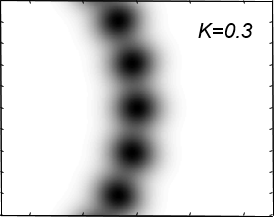
\includegraphics[width=\linewidth]{blanco2008efficient_fig17a}
		\caption{}
		\label{fig:blanco2008efficient_fig17a}
	\end{subfigure}
	\hfill
	\begin{subfigure}[t]{0.24\linewidth}
		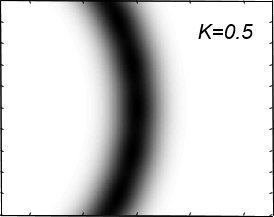
\includegraphics[width=\linewidth]{blanco2008efficient_fig17b}
		\caption{}
		\label{fig:blanco2008efficient_fig17b}
	\end{subfigure}
	\hfill
	\begin{subfigure}[t]{0.24\linewidth}
		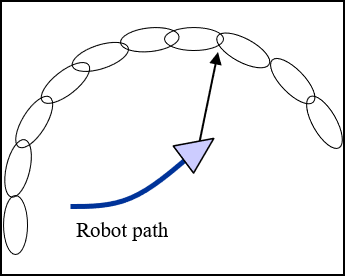
\includegraphics[width=\linewidth]{blanco2008efficient_fig10a}
		\caption{}
		\label{fig:blanco2008efficient_fig10a}
	\end{subfigure}
	\hfill
	\begin{subfigure}[t]{0.24\linewidth}
		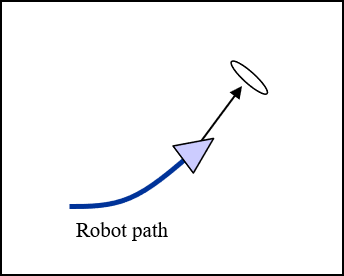
\includegraphics[width=\linewidth]{blanco2008efficient_fig10b}
		\caption{}
		\label{fig:blanco2008efficient_fig10b}
	\end{subfigure}
	\caption{Modellierung der ringförmigen Verteilung über radial angeordnete Normalverteilungen.}
	\label{fig:blanco2008efficient}
	\source{\cite{blanco2008efficientppt}}
\end{figure}


\begin{comment}
--------------------------------------------------------------------------------
- \cite{djugash2009robust}
	- A robust method of localization and mapping using only range
\end{comment}
\section{A robust method of localization and mapping using only range}

Jede bisherige Veröffentlichung die einen \Gls{roslam} mittels eines \Gls{ekf} umsetzen will, muss mit dem Problem der Linearisierung und der Multimodalität der Verteilung kämpfen. Hierfür wurde das Problem bisher immer im kartesischen Koordinatensystem betrachtet. Die Autoren dieses Werkes \cite{djugash2009robust} sind einen anderen Weg gegangen und haben das Problem ins Polarkoordinatensystem überführt. Dieses Vorgehen hat den großen Vorteil, dass ringförmige Verteilungen sehr gut im Polarkoordinatensystem modelliert werden können. Auch ist eine Vorverarbeitung (engl. Batch Process) der Entfernungsmessungen nicht mehr notwendig. Die Ergebnisse der Messung kann direkt an den Filter übergeben werden.

Wie bereits im Grundlagenkapitel besprochen besteht der Zustandsvektor eines \Gls{ekf} für die Lokalisierung aus der Pose (Position und Orientierung) des Roboters:

\[ q_k = \left[ x_k^r, y_k^r, \phi_k^r \right]^T. \]

Für das \Gls{slam} Problem muss der Zustandsvektor um die Positionen der Tags erweitert werden:

\[ q_k = \left[ x_k^r, y_k^r, \phi_k^r, x_k^1, y_k^1, \dots, x_k^N, y_k^N \right]^T. \]

Die Beschreibung des Zustandsvektors in Polarkoordinaten erfolgt dabei über die Festlegung der Mitte des Polarkoordinatensytems $\left( c_{x,k}, c_{y,k} \right)$ und über die Entfernung und den Winkel $\left( r_k, \theta_k \right)$:

\[ q_k = \left[ c_{x,k}^r, c_{y,k}^r, r_k^r, \theta_k^r, \phi_k^r, c_{x,k}^1, c_{y,k}^1, r_k^1, \theta_k^1, \dots, c_{x,k}^N, c_{y,k}^N, r_k^N, \theta_k^N \right]^T .~\footnote{Da für die Beschreibung der Zustände deutlich mehr Parameter benötigt werden, bezeichnet man dieses auch als relative Überparameterisierung (engl. \acrfull{rop}).}\]

Damit können alle Tags beschrieben werden, für den Roboter benötigt man aber noch den zusätzlichen Parameter $\phi_k^r$ um die Ausrichtung (engl. Heading) festzulegen.

Das vorherige Bewegungsmodell (engl. Motion Model) für das kartesischen Koordinatensystem kann weiterverwendet werden, nur die Parameterzuweisungen an $\left( c_{x,k}^r, c_{y,k}^r, \phi_k^r \right)$ ändern sich. Einzig das Messmodell (engl. Measurement Model) muss angepasst werden, um die erwartete Entfernung zu berechnen. Hierfür findet eine Konvertierung der Polarkoordinaten in Kartesische Koordinaten statt.

Die Abbildungen~\ref{fig:djugash2009robust_fig1} verdeutlichen zum einen, wie die Verteilung in Polarkoordinaten dargestellt wird und zum andern, wie mehrere Messungen miteinander kombiniert werden.

\autoref{fig:djugash2009robust_fig1a} beschreibt die tatsächliche Verteilung einer Einzelmessung. Das blaue Rechteck repräsentiert die Roboterposition und der rote Diamant die tatsächliche Tagposition. Die tatsächliche Verteilung einer Einzelmessung wird in Polarkoordinaten als grüne Fläche modelliert, siehe \autoref{fig:djugash2009robust_fig1b}. Über die blaue Ellipse wird die tatsächliche Verteilung mittels einer Normalverteilung angenähert und ergibt dabei die ringförmige Verteilung in der \autoref{fig:djugash2009robust_fig1c}.

Nachdem zwei Messungen von verschiedenen Positionen aus durchgeführt wurden, ergibt sich die tatsächliche Verteilung aus den beiden Schnittpunkten der Ringe, siehe \autoref{fig:djugash2009robust_fig1d}. Die Multimodalität der Verteilung kann über einen \Gls{ekf} nicht mehr abgebildet werden, daher wird zu diesem Zeitpunkt pro Verteilung ein eigener \Gls{ekf} angelegt. \autoref{fig:djugash2009robust_fig1e} beschreibt wie im vorherigen Abschnitt die tatsächlichen und angenäherten Verteilungen in Polarkoordinaten und \autoref{fig:djugash2009robust_fig1f} die Verteilung die sich aus der Annäherung der Verteilung ergibt.

\begin{figure}[h!]
	\centering
	\begin{subfigure}[b]{0.32\textwidth}
		\centering
		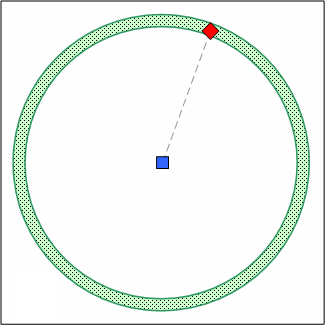
\includegraphics[width=\textwidth]{djugash2009robust_fig1a}
		\caption{}
		\label{fig:djugash2009robust_fig1a}
	\end{subfigure}
	\hfill
	\begin{subfigure}[b]{0.26\textwidth}
		\centering
		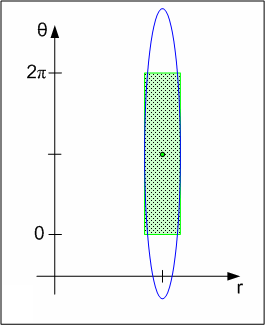
\includegraphics[width=\textwidth]{djugash2009robust_fig1b}
		\caption{}
		\label{fig:djugash2009robust_fig1b}
	\end{subfigure}
	\hfill
	\begin{subfigure}[b]{0.32\textwidth}
		\centering
		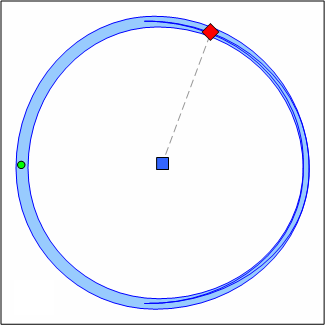
\includegraphics[width=\textwidth]{djugash2009robust_fig1c}
		\caption{}
		\label{fig:djugash2009robust_fig1c}
	\end{subfigure}
	\bigskip
		\begin{subfigure}[b]{0.32\textwidth}
		\centering
		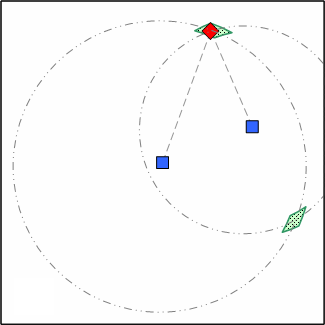
\includegraphics[width=\textwidth]{djugash2009robust_fig1d}
		\caption{}
		\label{fig:djugash2009robust_fig1d}
	\end{subfigure}
	\hfill
	\begin{subfigure}[b]{0.26\textwidth}
		\centering
		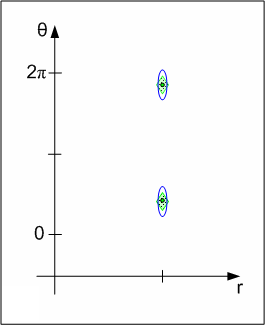
\includegraphics[width=\textwidth]{djugash2009robust_fig1e}
		\caption{}
		\label{fig:djugash2009robust_fig1e}
	\end{subfigure}
	\hfill
	\begin{subfigure}[b]{0.32\textwidth}
		\centering
		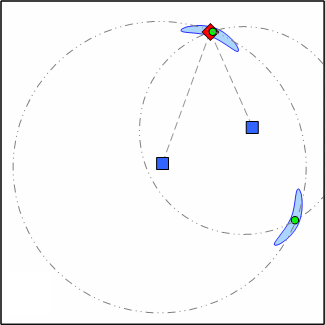
\includegraphics[width=\textwidth]{djugash2009robust_fig1f}
		\caption{}
		\label{fig:djugash2009robust_fig1f}
	\end{subfigure}
	\caption{Darstellung der tatsächlichen und angenäherten Verteilung in Kartesischen und Polarkoordinaten.}
	\label{fig:djugash2009robust_fig1}
	\source{\cite{djugash2009robust}}
\end{figure}


\begin{comment}
--------------------------------------------------------------------------------
- \cite{ahmad2011newstatevector}
	- A New State Vector for Range-Only SLAM
\end{comment}
\section{A New State Vector for Range-Only SLAM}


\begin{comment}
--------------------------------------------------------------------------------
- \cite{herranz2014comparison}
	- A Comparison of SLAM Algorithms with Range Only Sensors
\end{comment}
\section{A Comparison of SLAM Algorithms with Range Only Sensors}




\begin{comment}
------------------------------------------------------------------------------------------
\section{Übersicht der Meilensteine [Remove in final version]}

\begin{description}

\item[2001]
\begin{itemize}
\item !A solution to the simultaneous localization and map building (SLAM) problem (Zitiert von: 2803)
\item +Auxiliary variable based particle filters (115)
\item +Factor graphs and the sum-product algorithm (5869)
\item +Rao-Blackwellised particle filtering for dynamic Bayesian networks (1264)
\end{itemize}

\item[2002]
\begin{itemize}
\item +FastSLAM: A factored solution to the simultaneous localization and mapping problem (2469)
\item Indoor geolocation science and technology (985)
\end{itemize}

\item[2003]
\begin{itemize}
\item !Experimental results in range-only localization with radio (82)
\item !Pure range-only sub-sea SLAM (174)
\item +Recent results in extensions to simultaneous localization and mapping (18)
\end{itemize}

\item[2004]
\begin{itemize}
\item !Tracking moving devices with the cricket location system (547)
\item !A probabilistic approach to inference with limited information in sensor networks (42)
\item +An introduction to factor graphs (672)
\end{itemize}

\item[2006]
\begin{itemize}
\item !Simultaneous localization and mapping: part I (2982)
\item !Simultaneous localization and mapping (SLAM): Part II (1479)
\item Further results with localization and mapping using range from radio (69)
\item !Range-only slam for robots operating cooperatively with sensor networks (146)
\item !Range-only slam with interpolated range data (28)
\end{itemize}

\item[2007]
\begin{itemize}
\item !Application of UWB and GPS technologies for vehicle localization in combined indoor-outdoor environments (52)
\item +Rao-Blackwellized particle filter for multiple target tracking (264)
\end{itemize}

\item[2009]
\begin{itemize}
\item !Navigating with ranging radios: Five data sets with ground truth (18)
\item !Mobile robot localization based on ultra-wide-band ranging: A particle filter approach (90)
\item !Range-only SLAM with a mobile robot and a wireless sensor networks (109)
\end{itemize}

\item[2010]
\begin{itemize}
\item !Geolocation with range: Robustness, efficiency and scalability (11)
\item !Studying of WiFi range-only sensor and its application to localization and mapping systems (3)
\item !tinySLAM: A SLAM algorithm in less than 200 lines C-language program (62)
\end{itemize}

\item[2011]
\begin{itemize}
\item Ultra wide-band localization and SLAM: A comparative study for mobile robot navigation (17)
\item !A new state vector for range-only SLAM (10)
\end{itemize}

\item[2013]
\begin{itemize}
\item A Spectral Learning Approach to Range-Only {SLAM} (13)
\end{itemize}

\item[2014]
\begin{itemize}
\item !A comparison of slam algorithms with range only sensors (2)
\item !Efficient robot-sensor network distributed seif range-only slam (16)
\end{itemize}

\item[2015]
\begin{itemize}
\item ?Fusing ultra-wideband range measurements with accelerometers and rate gyroscopes for quadrocopter state estimation (30)
\end{itemize}

%\item[]
%\begin{itemize}
%\item 
%\end{itemize}

\end{description}
\end{comment}
	\begin{comment}
Fragestellung:
- Welche elektrische Beschaltung ist notwendig um das DWM1000 Modul von DecaWave in Betrieb nehmen zu können?
- Wie erfolgt die Entfernungsmessung zwischen den einzelnen UWB--Modulen?
- Wie erfolgt der Datenaustausch zwischen einem UWB--Modul und der Verarbeitungseinheit?
\end{comment}

\begin{comment}
------------------------------------------------------------------------------------------
Schmalbandkommunikation (engl. Narrowband)
Frequenzband (engl. Radio spectrum)
Frequenzspreizung (engl. spread spectrum)
Basisband (engl. Baseband)
https://en.wikipedia.org/wiki/Ultra-wideband
\end{comment}
\chapter{\glsentrylong{uwb}}
\label{ch:uwb}

Bei der normalen Funkübertragung werden die zu übermittelnden \Gls{basisband}signale auf eine sinusförmige Trägerfrequenz auf moduliert. Bei der \Gls{uwb}--Übertragung ist das nicht der Fall, die Signale werden im \Gls{basisband} übertragen. Hierfür werden im Nanosekundenbereich kurze Impulse erzeugt. \Gls{uwb}--Signale verwenden eine Bandbreite von bis zu \SI{500}{\MHz} und können im Frequenzbereich von \SIrange{3.6}{10.1}{\GHz} eingesetzt werden. Um zu verhindern das bestehende Dienste wie \Gls{gps} oder \Gls{wlan} gestört werden, wurde durch die \Gls{fcc} die maximale Abgabeleistung von \Gls{uwb}--Sendern stark begrenzt (unter \SI[per-mode=symbol]{-41.3}{\dBm\per\MHz}). Dadurch ist eine Koexistenz mit den bereits bestehenden Diensten möglich, ohne dass diese sich gegenseitig stören. \cite{win1998impulse, yang2004uwbcom, fontana2004recent, aiello2006ultra, yavari2014ultra}

Zu den bemerkenswerten Eigenschaften der \Gls{uwb}--Technologie zählt das verlustfreie Durchdringen von Hindernissen, präzise Entfernungsmessung im Zentimeterbereich, eine hohe Datenübertragungsrate von über \SI[per-mode=symbol]{110}{\mega\byte\per\second} in einem Bereich von \SIrange{10}{15}{\metre} und der geringe Energieverbrauch. \cite{yang2004uwbcom}

Die Einsatzgebiete werden dabei in die Klassen Bildgebende--, Kommunikation--, Mess-- und Fahrzeugradarsysteme unterteilt. Der Bereich der Bildgebendensysteme ist weiter unterteilt in Bodenradar, Medizinische Überwachung und Diagnostik und in Überwachungssysteme die Objekte durch Wände erkennen können. Kommunikations-- und Messsysteme werden ihrerseits unterteilt in Indoor-- und Outdoor--Systeme unterweilt. Hierzu zählen auch Systeme für die Navigation, Güternachverfolgung und Hochgeschwindigkeitsdatenübertragung. Die letzte Klasse wird in die Bereiche der Kollisionsvermeidung und Abstandssysteme unterteilt. \cite{yang2004uwbcom, lakkundi2006ultra, pan2007medical}


\begin{comment}
------------------------------------------------------------------------------------------
\end{comment}
\section{Historie}

Als Vater der \gls{uwb} Kommunikation kann der italienische Funkpionier Guglielmo Marconi angesehen werden. In den späten 1890er Jahren entwickelte er den Knallfunkensender, der über eine Funkenstrecke ein hochfrequentes Signal zur Übertragung von Morsezeichen erzeugt. Mit dieser Apparatur gelang es Ihm, im Jahre 1901 einen Nachrichtenaustausch zwischen Nordamerika und Europa über den Nordatlantik durchzuführen.\cite{fontana2004recent}

% Weitere Quellen:
% http://www.ieee.ca/millennium/radio/radio_differences.html
% https://de.wikipedia.org/wiki/Knallfunkensender

Bis in die Anfänge der 1960er Jahre dominierte jedoch die sinusförmige Funkübertragungsform. Dies änderte sich als die Forscher vom \gls{llnl} und \gls{lanl} begangen die Ausbreitung elektromagnetischer Wellen nicht zur im Frequenz- sondern auch im Zeitbereich zu untersuchen. Grundlegende Erkenntnisse wurden dabei im Bereich der Impulssender, -empfänger und -antennen gesammelt.\cite{eltaher2004positioning, fontana2004recent, lakkundi2006ultra, aiello2006ultra}

% TODO: time-domain sampling oscilloscopes
Durch die Einführung der zeitbereichsbasierten Abtastoszilloskope im Jahre 1962 durch Tektronix bzw. Hewlett-Packard war es zum ersten Mal möglich eine \gls{uwb} Wellenform aufzufangen und anzuzeigen. Ermöglicht wurde dies erst durch den Einsatz von Tunneldioden und Avalanchetransistoren. \cite{fontana2004recent, lakkundi2006ultra, aiello2006ultra}

Ab dem Jahre 1964 produzierten beide Hersteller Messgeräte für die Diagnose im Zeitbereich. \cite{barrett2001technical}

Ab den Anfängen der 1970er Jahre waren alle wichtigen Grundsteine für ein \gls{uwb} System für Kommunikation- bzw. Radaranwendungen gelegt. Dazu zählten auch diverse eingereichte Patente von Harmuth an der \gls{cua}, Ross und Robbins bei der Sperry Rand Corporation und Paul van Etten an der \gls{usaf} im Rome Air Development Center.\cite{barrett2001technical, fontana2004recent, yang2004uwbcom} Hervorzuheben ist das eingereichte Patent von Ross im Jahre 1973, siehe \cite{g1973transmission}.

% INFO:
% Rome Laboratory (Rome Air Development Center until 1991) is the US
% "Air Force 'superlab' for command, control, and communications"[4] research and
% development and is responsible for planning and executing the USAF science and
% technology program.

% TODO: Warum ist gerade diese Patent hervorzuheben?
% US 3728632 A
% Transmission and reception system for generating and receiving base-band pulse
% duration pulse signals without distortion for short base-band communication system
% Veröffentlichungsnummer: US3728632 A
% Publikationstyp: Erteilung
% Veröffentlichungsdatum	: 17. Apr. 1973
% Eingetragen: 12. März 1971
% Erfinder:	Ross G
% Ursprünglich Bevollmächtigter: Sperry Rand Corp
% ZUSAMMENFASSUNG
% An electromagnetic signal communication system utilizing short base-band pulse
% signals of sub-nanosecond duration employs dispersionless, broad band antenna
% transmission line elements for generating and preserving the character of the
% short base-band pulses in respective transmitter and receiver sub-systems.

Kurz darauf im Jahre 1974 wurde die \gls{uwb} Technologie kommerziell erfolgreich von Morey bei der \gls{gssi} für ein Bodenradar (engl. \acrfull{gpr}) angewendet. \cite{barrett2001technical}

Im Zeittraum von 1977 bis 1989 wurden mehrere Programme und Workshops organisiert um die Entwicklung von \gls{uwb} Systemen voranzutreiben, darunter auch bei der \gls{usaf} und dem \gls{usdod}. Ebenfalls gab es mehrere akademische Programme an diversen Instituten, darunter auch am \gls{llnl}, \gls{lanl}, University of Michigan, University of Rochester und
Polytechnic University, mit dem Fokus auf den physikalischen Unterschieden zwischen der Kurzimpulsübertragung und den Langimpulssignalen bzw. kontinuierlichen Impulssignalen bei der Interaktion mit verschiedenen Materialien.\cite{barrett2001technical}

% TODO: Der letzte Satz ist zu lang. Aufspalten!

Ab dem Jahre 1989 wurde der Name \gls{uwb}\footnotemark{} durch das \gls{usdod} geprägt. Diese Definition galt für alle Geräte die mindestens eine Bandbreite von \SI{1.5}{\GHz} bzw. \SI{25}{\percent} der \gls{fbw} belegten. \cite{eltaher2004positioning, fowler1990assessment, yang2004uwbcom, aiello2006ultra, fontana2004recent}

\footnotetext{Vorher war die \gls{uwb} Technologie nur unter den Synonymen ``baseband communication'', ``carrier free communication'', ``impulse radio'', ``large relative bandwidth communication'', ``nonsinusoidal communication'', ``orthogonal functions'', ``sequency theory'', ``time domain'', ``large-relative-bandwidth radio/radar signals'', ``video-pulse transmission'' und/oder ``Walsh waves communication'' bekannt.}


% TODO: Fachbegriffe Übersetzen?

% TODO: Sollen die Militärischen Anwendungfälle erwähnt werden? Vielleicht besser bei der FCC regulierung.
% Das Militär hatte dabei für sich die Anwendungsfälle im Bereich Radar und hochsicherheitskommunkation entdeckt.\cite{eltaher2004positioning}

Im Jahre 1994 wurde von McEwan an der \gls{llnl} das \gls{mir} konstruiert. Hierbei handelte es sich um ein \gls{uwb} Radarsystem mit bemerkenswerten Eigenschaften. Das Radarsystem verfügte über eine sehr hohe Signalsensitivität, einen kompakten Aufbau, eine kostengünstige Herstellung und einen sehr geringen Energieverbrauch, der sich im Bereich von Mikrowatt befanden und daher ideal für batteriebetriebene Anwendung eignete. \cite{barrett2001technical}

% TODO: Zwei mal bemerkenswerte Eigenschaften. Korrigieren bzw. Umformulieren!!!

Vor dem Jahre 2002 war die Verwendung von \gls{uwb} auf Radarssytem beschränkt, die größtenteils in militärischen Anwendungen aufzufinden waren. \cite{yang2004uwbcom} Das änderte sich ab dem Jahre 1998, als die \gls{fcc} mit der Standardisierung der \gls{uwb} Nutzung begann. Im Jahre 2002 wurden durch die \gls{fcc} in den Vereinigten Staaten von Amerika große Frequenzbereiche (\SIrange{3.6}{10.1}{\GHz}) für die kommerzielle Nutzung freigegeben hat, siehe First Report and Order (R\&O). Danach wurden erstmals auch eine nicht militärische Anwendung im Bereich ``Imaging systems'', ``communication and measurement systems'' und ``vehicular radar systems'' möglich. \cite{yang2004uwbcom}

% TODO: Zitieren des FCC R&O
% [12] FCC First Report and Order: In the matter of Revision of Part 15 of the
% Commission’s Rules Regarding Ultra-Wideband Transmission Systems,
% FCC 02–48, April 2002.
% Chrome: g FCC 02-48 bibtex
% https://transition.fcc.gov/Bureaus/Engineering_Technology/Orders/2002/fcc02048.pdf

Weitere Staaten folgten der \gls{fcc} Regulierung/Standardisierung und gaben ebenfalls große Frequenzbereiche für die \gls{uwb} Technologie frei. Details zu den Regularien der einzelnen Staaten können unter \cite{decawave2015uwbreg} eingesehen werden.

	
\begin{comment}
------------------------------------------------------------------------------------------
- Welche alternativen Technologien gibt es zu UWB?
- Einen guten Überblick über die Eigenschaften der Drahtlosen-Protokolle (engl. Wireless Protocols) Bluetooth, UWB, ZigBee und WiFi liefert die Arbeit \cite{lee2007comparative} von \citeauthor{lee2007comparative}.
	- Bluetooth
		- Piconet/Scatternet
		- low data rate
		- small data sizes (around smaller than 339 bytes)
		- is the most complicated protocol with 188 primitives and events in total
		- intended for portable products, short ranges, and limited battery power.
	- ZigBee
		- supporting simple devices that consume minimal power and typically operate in the personal operating space (POS) of 10m.
		- full-function device (FFD) and a reduced-function device (RFD)
		- low data rate
		- highest transmission time
		- data size smaller than 102 bytes
		- is the simplest one with only 48 primitives
		- the simplicity makes ZigBee very suitable for sensor networking applications due to their limited memory and computational capacity.
		- intended for portable products, short ranges, and limited battery power.
	- UWB
		- Indoor short-range high-speed wireless communication
		- high data rate
		- lowest transmission time
		- large data sizes much better efficiency
		- proposed for shortrange and high data rate applications.
		- have better efficiency in energy consumption.
	- WiFi
		- allows users to surf the Internet at broadband speeds when connected to an access point (AP) or in ad hoc mode.
		- high data rate
		- large data sizes much better efficiency
		- designed for a longer connection and supports devices with a substantial power supply
		- have better efficiency in energy consumption.
- For a wireless sensor network in factory automation systems, since most data size of industrial monitoring and control are generally small, (e.g. the temperature data in an environmental monitoring may required less than 4 bytes only), Bluetooth and ZigBee protocols may be a good selection (from a data coding efficiency point of view) in spite of their slow data rate.
- Welche Eigenschaften haben die alternativen Technologien?
- Warum hab ich mich für UWB entschieden?
\end{comment}
%\section{Alternative Technologien/Gegenüberstellung}


\begin{comment}
------------------------------------------------------------------------------------------
\end{comment}
\section{Erstellte Hardware}

\begin{comment}
------------------------------------------------------------------------------------------
- Datenübertragung zum Host
- Batteriebetrieb
- TODO: Erweiterbare Hardwareplattform
\end{comment}
\subsection{Anforderungen}

An die zu erstellende Hardware werden mehrere Anforderungen gestellt.

Um eine Entfernungsmessung durchzuführen wird immer ein \Gls{tag} und mindestens ein \Gls{anchor} benötigt. Sowohl der \Gls{tag} als auch der \Gls{anchor} sollen aus den gleichen elektrischen Komponenten bestehen, also eine gemeinsame Hardwareplattform bilden. Die unterschiedliche Funktionalität pro Modul soll sich dann aus verschiedenen Software-Ständen der Firmware herausbilden.

Die \Gls{anchor} sollen im Bedarfsfall frei im Raum verteilt werden können. Nicht an jeder Stelle steht eine Stromversorgung zur Verfügung, daher muss jedes Modul über eine separate Energiequelle verfügen.

Zusätzlich muss der \Gls{tag} über eine bidirektionale Kommunikationsschnittstelle zur Verarbeitungseinheit verfügen. Über diese sollen zum einen Steuerbefehle an das \Gls{uwbm} geschickt werden und zum anderen sollen die gemessenen Entfernungen zwischen dem \Gls{tag} und den \Glspl{anchor} an die Verarbeitungseinheit übertragen werden.


\begin{comment}
------------------------------------------------------------------------------------------
- Zusätzlich werden Erfahrungsberichte aus dem Internet ausgewertet um die Beschaltung weiter zu verfeinern, siehe \cite{Trojer2015, Holder2016, Holder2016a}.
\end{comment}
\subsection{Hardware Zusammenstellung}


\begin{comment}
------------------------------------------------------------------------------------------
TODO: Wie wird der Vorwiderstand berechnet? ca. 10mA bei 1.8V, R=(U_0-U_LED)/I_LED

LED Vorwiderstand berechnen
	- https://www.youtube.com/watch?v=iNZj91TSRUg
	- DW1000 Datasheet - 5.9 General Purpose Input Output (GPIO)
\end{comment}
\subsubsection{\glsentrylong{uwbt}}\label{subsec:uwb_transceiver}

Als \Gls{uwbt} werden die Komponenten der Firma \textit{DecaWave} verwendet. Bei dem \textit{DW1000} handelt es sich nur um dem \Gls{ic} der für das Erzeugen und Verarbeiten der \gls{uwb}--Funksignale zuständig ist. Der \textit{DWM1000} beinhaltet neben dem \textit{DW1000} auch die notwendige Beschaltung und zusätzlich eine Antenne für die Übertragung, siehe \figurename~\ref{fig:pin_assignment}.

\begin{figure}
	\begin{subfigure}[t]{0.4\textwidth}
		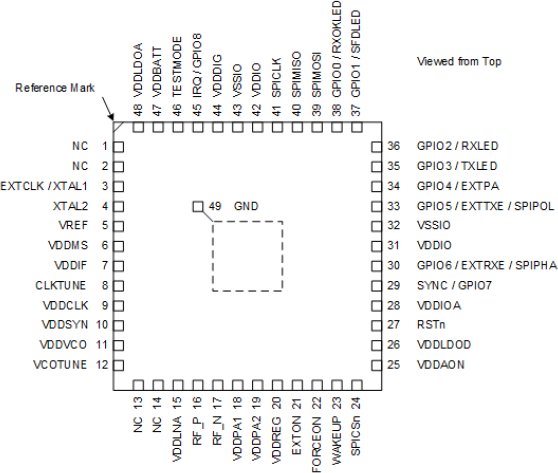
\includegraphics[width=\textwidth]{dw1000_pin_assignments.png}
		\caption{DW1000 \gls{ic}}
		\label{fig:dw1000_pin_assignments}
		\source{\cite{decawave2016dw1kdatasheet}}
	\end{subfigure}
	\hfill
	\begin{subfigure}[t]{0.4\textwidth}
		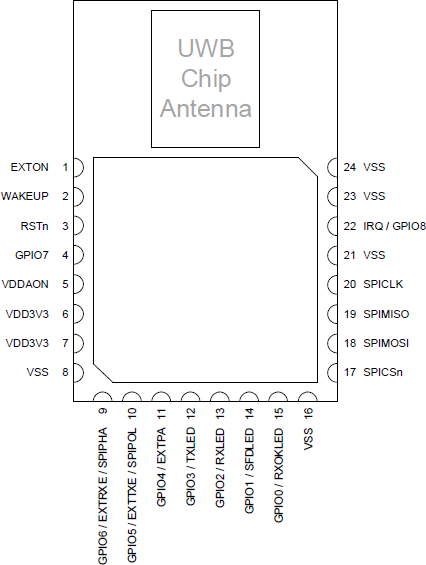
\includegraphics[width=\textwidth]{dwm1000_pin_assignments.png}
		\caption{DWM1000 Modul}
		\label{fig:dwm1000_pin_assignments}
		\source{\cite{decawave2016dwm1kdatasheet}}
	\end{subfigure}
	\caption{DecaWave \gls{ic} Pin Belegung}
	\label{fig:pin_assignment}
\end{figure}

Der \textit{DWM1000} kann mit einer Spannung von \SIrange{2.8}{3.6}{\volt}\cite{decawave2016dwm1kdatasheet} betrieben werden, idealerweise mit \SI{3.3}{\volt}. Das bedeutet aber auch, dass die Logikpegelspannung für die \gls{spi} Schnittstelle \SI{3.3}{\volt} beträgt. Dieser Umstand muss bei der Auswahl des Mikrocontrollers berücksichtigt werden.

Die Kommunikation mit dem \textit{DWM1000} erfolgt über die \gls{spi} Schnittstelle, hierfür sind die Pins \gls{sclk}, \gls{mosi}, \gls{miso} und \gls{ss} zu verwenden \cite{decawave2016dwm1kdatasheet}. Bei der \gls{spi}--Schnittstelle handelt es sich um eine Master-Slave Architektur, das bedeutet das Daten vom Master gesendet und angefragt werden können. Der Slave kann jedoch nur Daten auf Anfrage senden. Um zu verhindern, dass der Master periodisch auf das Eintreffen einer Nachricht anfragen muss, kann der \gls{irq}--Pin des Slaves verwendet werden. Um zu verhindern das kurzfristige Spannungsspitzen einen Interrupt auslösen, muss der \gls{irq}--Pin über einen Pulldown--Widerstand auf Masse gezogen werden.

Um das \textit{DWM1000} erfolgreich zu initialisieren muss der RSTn--Pin durch den Mikrocontroller angesteuert werden. Zusätzlich ergibt sich, über die Beschaltung dieses Pins, die Möglichkeit den \textit{DWM1000} per Hardware im laufenden Betrieb neu zu starten.

Zusätzliche Informationen, wie der Versand und Empfang von Nachrichten, könnten über Status--Leuchtdioden ausgegeben werden. Hierfür wird jeder der Pins GPIO1 bis GPIO3 jeweils mit einem Vorwiderstand und einer Leuchtdiode verbunden.


\begin{comment}
------------------------------------------------------------------------------------------
\end{comment}
\subsubsection{Mikrocontroller}

Wie bereits im Abschnitt~\ref{subsec:uwb_transceiver} erwähnt beträgt die Logikpegelspannung \SI{3.3}{\volt}. Durch diesen Umstand entfallen alle Mikrocontroller die mit einer \SI{5}{\volt} Versorgungsspannung, wie z.B. der beliebte Arduino Uno, betrieben werden. Die Entscheidung fiel auf den \textit{Pro Trinket} der Firma \textit{Adafruit}, der als Hauptprozessor den \Gls{atmega} verwendet. Dieser hat den Vorteil, dass er jeweils in einer \SI{5}{\volt} und \SI{3.3}{\volt} Variante existiert. Zusätzlich ist die \SI{3.3}{\volt} Variante mit einem Systemtakt von \SI{12}{\MHz} schneller als der vergleichbare Arduino Pro Mini \SI{3.3}{\volt} der nur mit \SI{8}{\MHz} getaktet ist.

%\begin{wrapfigure}{r}{0.5\textwidth}
\begin{figure}[!h]
	\centering
	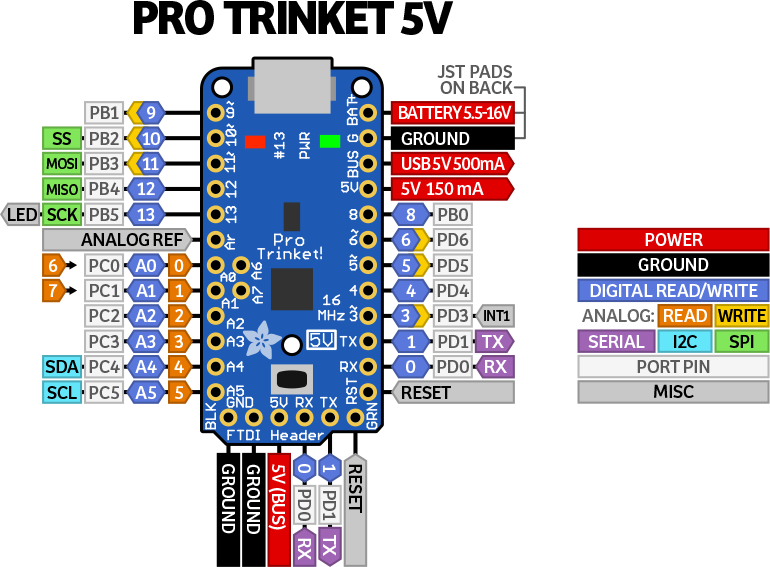
\includegraphics[width=0.5\textwidth]{adafruit_pro_trinket_5v.png}
	\caption[Adafruit Pro Trinket]{Adafruit Pro Trinket\protect\footnotemark}
	\label{fig:adafruit_pro_trinket}
	\source{\cite{adafruit2014protrinket}}
\end{figure}

\footnotetext{Der \textit{Adafruit Pro Trinket} \SI{3.3}{\volt} ist zum Großteil pinkompatibel zu der \SI{5}{\volt} Variante. Nur der Pin \textit{BAT+} benötigte eine Batteriespannung von \SIrange{3.5}{16}{\volt} und der drei Reihen weiter unten liegende \SI{5}{\volt} Pin liefert nur \SI{3.3}{\volt}.}

Um eine Kommunikationsverbindung zwischem dem \textit{DWM1000} und dem Mikrocontroller herzustellen, müssen die Pins anhand der \tablename~\ref{tab:pin_assignment_between_dwm1k_and_pro_trinket} verbunden werden.

\begin{table}
	\centering
	\begin{tabular}{||c|c|c||} 
		\hline
		DWM1000 (Pin)&Pro Trinket (Pin)&Bedeutung\\\hline
		\hline
		SPICLK (20)&SCK (13)&SPI\\\hline
		SPIMISO (19)&MISO (12)&SPI\\\hline
		SPIMOSI (18)&MOSI (11)&SPI\\\hline
		SPICSn (17)&SS (10)&SPI\\\hline
		\hline
		IRQ (22)&INT1 (3)&Interrupt\\\hline
		\hline
		RSTn (3)&PB1 (9)&Hardware Reset\\\hline
	\end{tabular}
	\caption{Pinbelegung zwischen dem \textit{DWM1000} und \textit{Pro Trinket}.}
	\label{tab:pin_assignment_between_dwm1k_and_pro_trinket}
\end{table}


\begin{comment}
% Lithium Ion Cylindrical Battery - 3.7v 2200mAh
% https://www.adafruit.com/product/1781
% Lithium Ion Polymer Battery - 3.7v 2500mAh
% https://www.adafruit.com/product/328
% Adafruit Pro Trinket LiPoly/LiIon Backpack
% https://learn.adafruit.com/adafruit-pro-trinket-lipoly-slash-liion-backpack?view=all
------------------------------------------------------------------------------------------
\end{comment}
\subsubsection{Energieversorgung}

Um den \Gls{uwbt} und den \textit{Pro Trinket} mit Energie zu versorgen wird ein Lithium--Ionen Akku mit einer Spannung von \SI{3.7}{\volt} und einer Kapazität von \SI{2200}{\mAh} verwendet. Die Verbindung zwischen den beiden wird über einen Lithium--Ionen Akku Lade--Chip hergestellt. Diesen gibt es als fertiges Modul von \textit{Adafruit} mit der Bezeichnung \textit{Pro Trinket LiPoly/LiIon Backpack}.

Bevor jedoch dieses Modul eingesetzt werden kann, müssen noch zwei Modifikationen durchgeführt werden. Zum einen kann die Energiequelle mittels eines Schalters vom Verbraucher getrennt werden. Per Standard sind jedoch diese zwei Pins mit einander verbunden und müssen mit einem scharfen Messer unterbrochen werden, siehe \figurename~\ref{fig:pro_trinket_liion_backpack_top}. Zum anderen wird der Lithium--Ionen Akku nur mit einem Strom von \SI{100}{\mA} geladen. Bei einer Kapazität von \SI{2200}{\mAh} würde ein vollständiger Ladezyklus ca. \SI{22}{\hour} dauern. Um diese Zeit zu verkürzen, müssen die zwei Lötpads, siehe \figurename~\ref{fig:pro_trinket_liion_backpack_bottom}, miteinander verbunden werden. Danach wird der Lithium--Ionen Akku mit einem Strom von \SI{500}{\mA} geladen und dementsprechend verkürzt sich die Ladedauer auch auf ca. \SI{2.5}{\hour}.
%TODO: 2.5 Stunden? Häh? Wie wäre es mit 2 1/2, laut Duden korrekt.

\begin{figure}
	\centering
	\begin{subfigure}[t]{0.3\linewidth}
		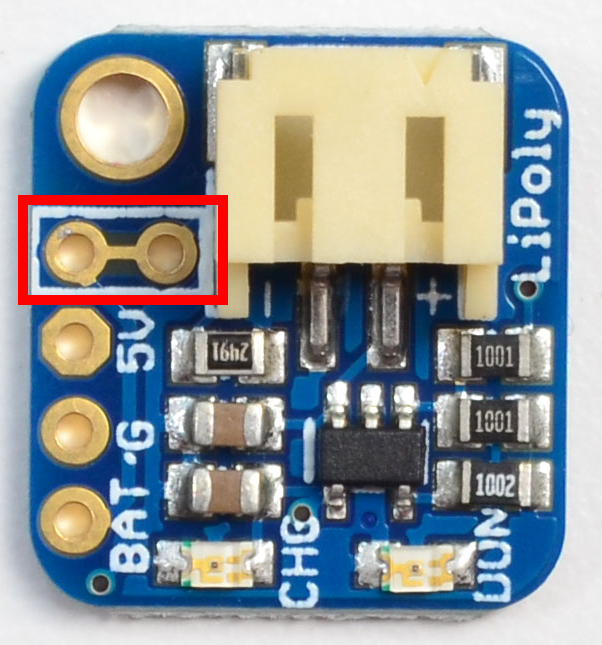
\includegraphics[width=\linewidth]{adafruit_lipoly_backpad_top_with_marker}
		\caption{Modifikation für den Schalter.}
		\label{fig:pro_trinket_liion_backpack_top}
	\end{subfigure}
	\qquad
	\begin{subfigure}[t]{0.3\linewidth}
		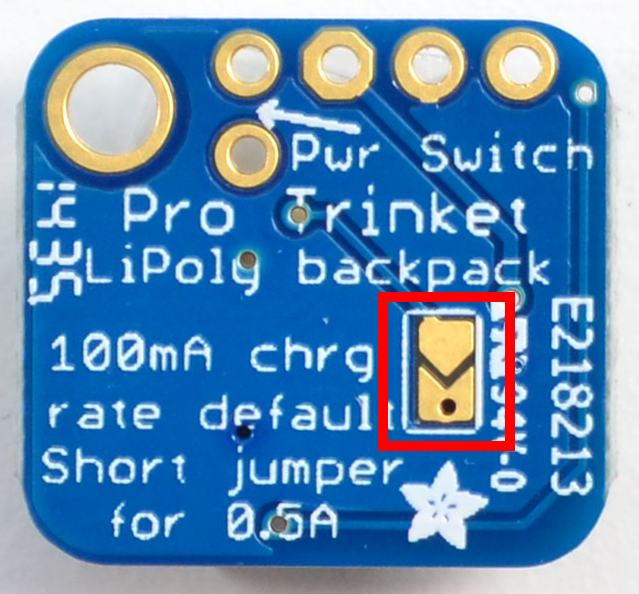
\includegraphics[width=\linewidth]{adafruit_lipoly_backpad_back_with_marker}
		\caption{Modifikation für einen höheren Ladestrom.}
		\label{fig:pro_trinket_liion_backpack_bottom}
	\end{subfigure}
	\caption{Adafruit Pro Trinket LiPoly/LiIon Backpack}
	\source{\cite{adafruit2014liionbackpack}}
	\label{fig:pro_trinket_liion_backpack}
\end{figure}

Um eine Verbindung zwischen dem \textit{Pro Trinket LiPoly/LiIon Backpack} und dem \textit{Pro Trinket} herzustellen, müssen die Pins anhand der \tablename~\ref{tab:pin_assignment_between_liion_backpack_and_pro_trinket} verbunden werden.

\begin{table}
	\centering
	\begin{tabular}{||c|c|c||} 
		\hline
		LiIon Backpack&Pro Trinket&Bedeutung\\\hline
		\hline
		BAT & BAT+ & Batteriespannung\\\hline
		5V & BUS & Ladespannung\\\hline
		G & GND & Masse\\\hline
		\hline
		SW1 & -- & Schalter\\\hline
		SW2 & -- & Schalter\\\hline
	\end{tabular}
	\caption{Pinbelegung zwischen dem LiIon Backpack und dem Pro Trinket.}
	\label{tab:pin_assignment_between_liion_backpack_and_pro_trinket}
\end{table}

Um den Lithium--Ionen Akku zu laden, bedarf es nicht mehr als den \Gls{usb}--Stecker des \textit{Pro Trinket} mit dem Computer oder einem \Gls{usb}--Ladegerät zu verbinden.


\begin{comment}
------------------------------------------------------------------------------------------
% Adafruit CP2104 Friend - USB to Serial Converter
% https://www.adafruit.com/product/3309
% https://www.silabs.com/documents/public/data-sheets/cp2104.pdf
% Universal Asynchronous Receiver Transmitter
% https://de.wikipedia.org/wiki/Universal_Asynchronous_Receiver_Transmitter
\end{comment}
\subsubsection{Datenaustausch}

% TODO: Computer? PC? Verarbeitungseinheit?
Der \Gls{atmega} verfügt nicht über einen eingebauten \Gls{usb}--Controller, daher ist ein direkter Datenaustausch zwischen dem Mikrocontroller und einem Computer nicht möglich. Jedoch verfügt der \Gls{atmega} über eine \gls{uart}--Schnittstelle, mit der Daten seriell über die Pins RX und TX übertragen und empfangen werden können. Mittels eines zusätzlichen Moduls kann diesen Datenstrom aufgefangen und über die \Gls{usb}--Schnittstelle übertragen werden. Der \textit{CP2104 Friend} von \textit{Adafruit} erledigt genau diese Aufgabe. Angeschlossen wird er über den \gls{ftdi}--Header, siehe \figurename~\ref{fig:adafruit_pro_trinket}. Dadurch ist es möglich die \Gls{uwbm} die einen Datenaustausch benötigen mit einem entsprechenden Modul auszurüsten.

% TODO: In jedem Abschnitt der gleiche Satz :$
Um eine Verbindung zwischen dem \textit{CP2104 Friend} und dem \textit{Pro Trinket} herzustellen, müssen die Pins anhand der \tablename~\ref{tab:pin_assignment_between_cp2104_and_pro_trinket} verbunden werden.

\begin{table}
	\centering
	\begin{tabular}{||c|c|c||} 
		\hline
		CP2104 Friend & Pro Trinket & Bedeutung\\\hline
		\hline
		GND & GND & Masse\\\hline
		CTS & GND & Masse\\\hline
		\hline
		5V & 5V & Versorgungsspannung\\\hline
		\hline
		TXD & RXD & Datenaustausch\\\hline
		RXD & TXD & Datenaustausch\\\hline
		\hline
		RTS & RTS & Reset\\\hline
	\end{tabular}
	\caption{Pinbelegung zwischen dem \textit{CP2104 Friend} und dem \textit{Pro Trinket}.}
	\label{tab:pin_assignment_between_cp2104_and_pro_trinket}
\end{table}


\begin{comment}
- Kosten für den Aufbau
------------------------------------------------------------------------------------------
\end{comment}
\subsubsection{Materialkosten pro \glsentrytext{uwbm}}

Die Materialkosten für einen \gls{tag} betragen jeweils \SI{45.15}{\euro} und für einen \gls{anchor} \SI{56.24}{\euro}. Der Unterschied ergibt sich dadurch, dass z.B. für einen \gls{tag} kein Lithium--Ionen Akku benötigt wird, da dieser von der Energiequelle des Roboters gespeist wird.
Die detaillierte Auflistung der Materialkosten können in der \tablename~\ref{tab:kosten_pro_modul} nachgeschlagen werden. Die Bauelemente die jeweils für einen \gls{tag} bzw. \gls{anchor} benötigt werden, sind in der dazugehörigen Spalte angekreuzt.


\begin{comment}
- Schaltplan-Skizze
	- Besonderheiten (NetLabels)
	- SVG/PNG/PDF-Export
	- Gruppierung nach Funktionsgruppen
------------------------------------------------------------------------------------------
\end{comment}
\subsubsection{Schaltplan} \label{subsec:schaltplan_uwb_modul}

Eine Übersicht der besprochenen Bauelemente, gruppiert nach Funktionsgruppen, können dem Schaltplan in \figurename~\ref{fig:schaltplan_uwb_modul} entnommen werden.

\begin{figure}
	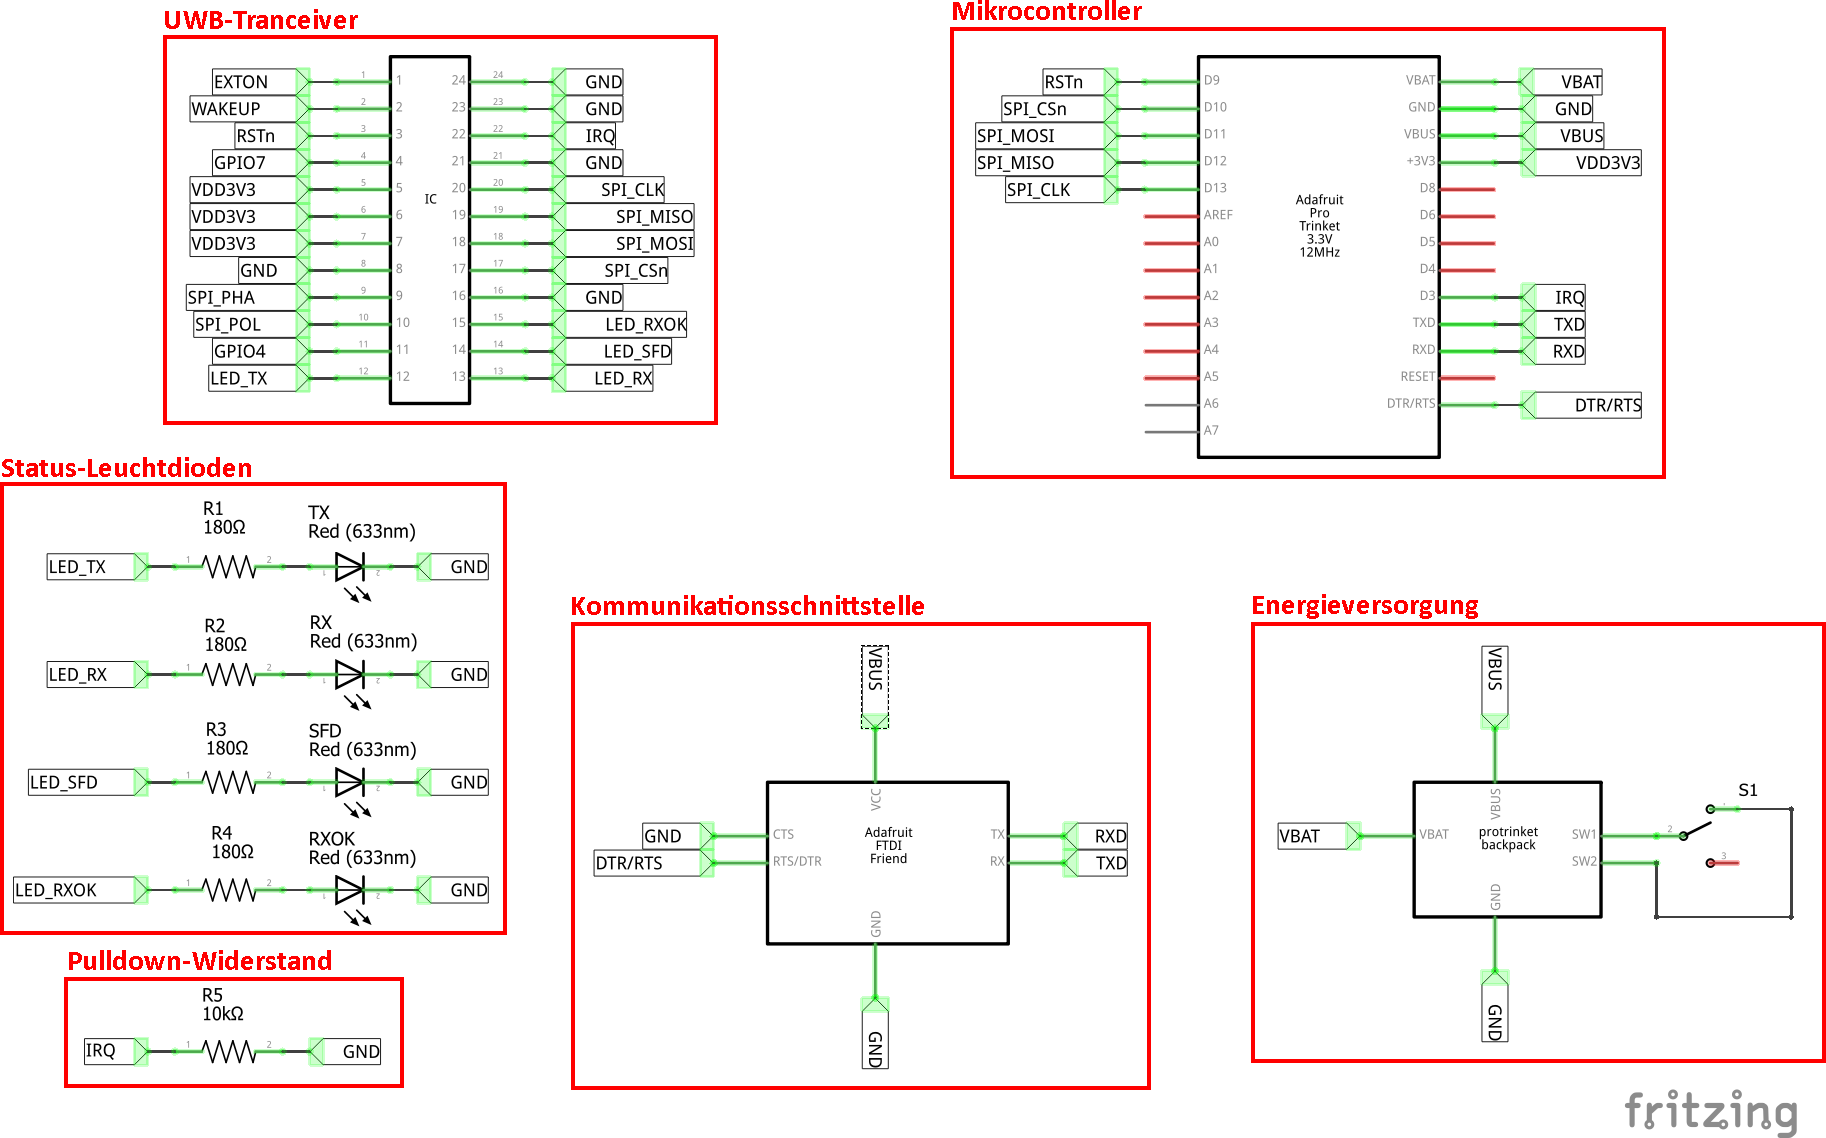
\includegraphics[width=\textwidth]{Trinket_And_DWM1000_v3_schem}
	\caption{Schaltplan des \Glsuserii{uwbm}.}
	\label{fig:schaltplan_uwb_modul}
\end{figure}


\begin{comment}
------------------------------------------------------------------------------------------
- 1. Prototyp Aufbau auf einem Breadboard
	- UWB-Adapter von ...?
	- SMD Löttechnik
	- Funktionstest
	- Skript als Anhang
- 2. Prototyp Aufbau auf einem Lochstreifen
	- Kommunikations- und Entfernungsmessungstest
\end{comment}
\subsection{Prototypen}

Anhand des vorläufigen Schaltplans wurden zwei Prototypen erstellt, siehe \figurename~\ref{fig:prototypen_der_uwb_module}.

Der erste Prototyp wurde auf einer Steckplatine realisiert, siehe \figurename~\ref{fig:prototyp_eins_uwb_modul}. Die elektrische Verbindung zu dem \textit{DWM1000} wurde dabei über eine Freiluftverdrahtung mit einem steckplatinenfähigen Adapter umgesetzt. Der erste Verbindungsaufbau wurde dabei mit dem Beispielprogramm \textit{BasicConnectivityTest} aus dem GitHub--Projekt \cite{Trojer2015} durchgeführt. Hierbei ist zu beachten das der \textit{PIN\_IRQ} bei dem \textit{Pro Trinket} nicht auf Pin 2 sondern auf Pin 3 liegt.

Während dem Aufbau des ersten Prototypen wurde ein \Gls{pcb}--Adapterboard, siehe \figurename~\ref{fig:pcb_dwm1000_adapterboard_top}, für den \textit{DWM1000} bestellt. Dieses \gls{pcb}--Adapterboard wurde ebenfalls dem GitHub--Projekt \cite{Trojer2015} entnommen. Mit diesem wurde dann ein zweiter Prototyp aufgebaut, siehe \figurename~\ref{fig:prototyp_zwei_uwb_modul}, der zusätzlich ohne eine externe Energieversorgung betrieben werden konnte. Mittels der beiden Prototypen war ein erster Nachrichtenaustausch bzw. eine erste Entfernungsmessung möglich. Der Nachrichtenaustauch wurden mit den Beispielprogrammen \textit{BasicReceiver} und \textit{BasicSender} erprobt, die Entfernungsmessung mit \textit{RangingAnchor} und \textit{RangingTag}.

\begin{figure}
	\begin{subfigure}[t]{0.4\textwidth}
		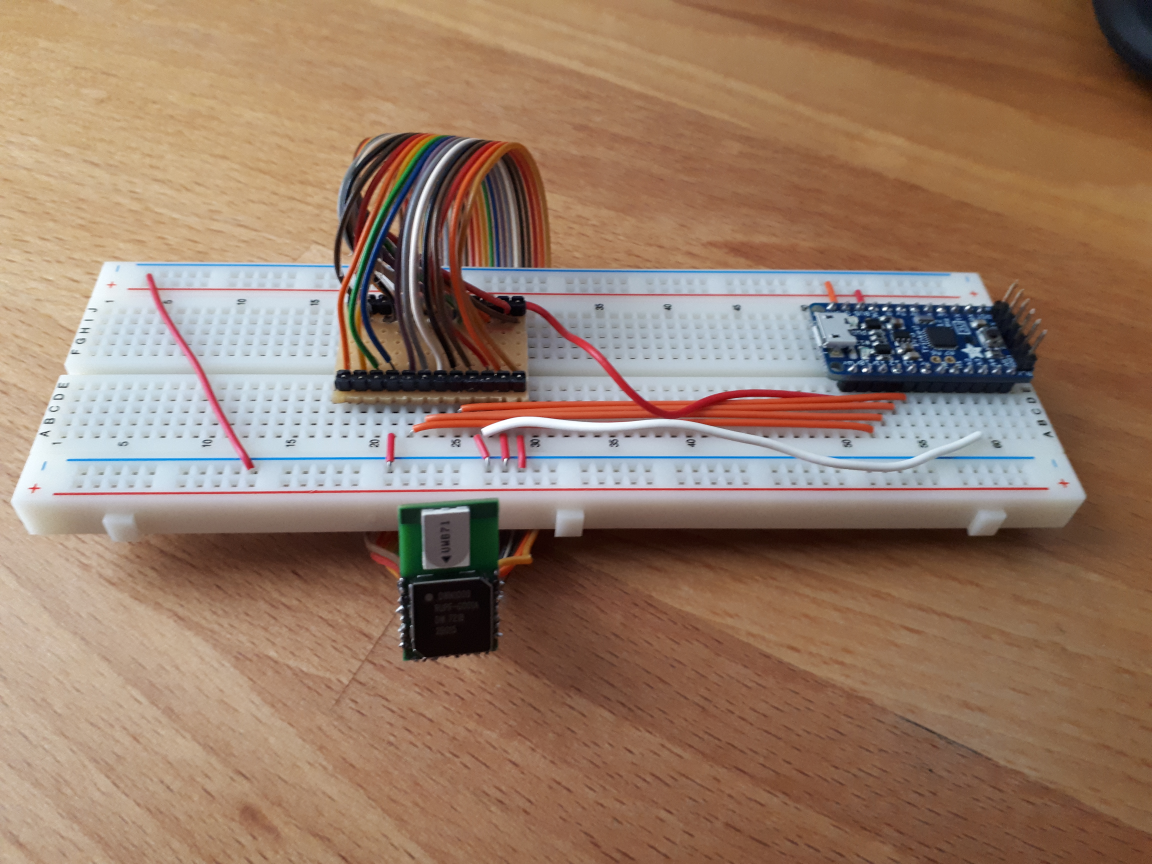
\includegraphics[width=\textwidth]{prototyp_eins_uwb_modul}
		\caption{Erster Prototyp auf einer Steckplatine.}
		\label{fig:prototyp_eins_uwb_modul}
	\end{subfigure}
	\hfill
	\begin{subfigure}[t]{0.4\textwidth}
		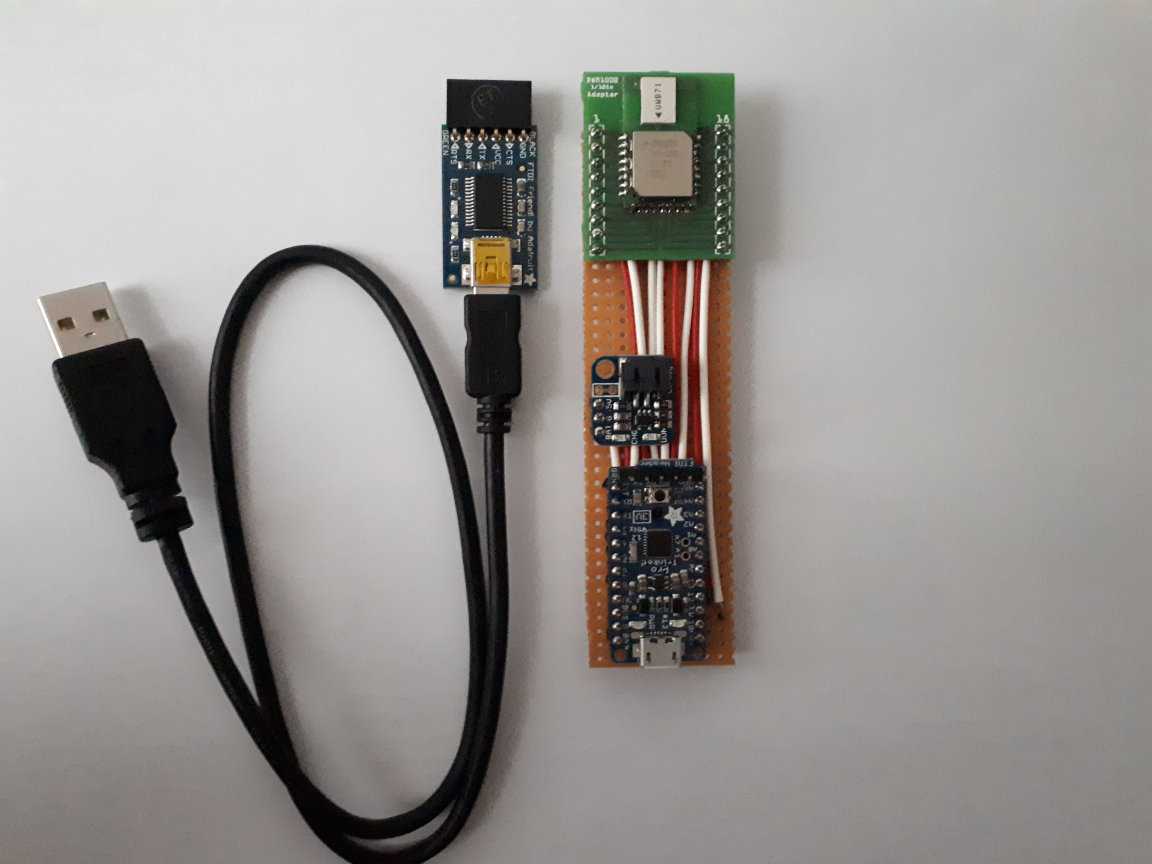
\includegraphics[width=\textwidth]{prototyp_zwei_uwb_modul}
		\caption{Zweiter Prototyp auf einem Lochstreifen.}
		\label{fig:prototyp_zwei_uwb_modul}
	\end{subfigure}
	\caption{Die ersten zwei Prototypen der \glspl{uwbm}.}
	\label{fig:prototypen_der_uwb_module}
\end{figure}

\begin{figure}
  \centering
  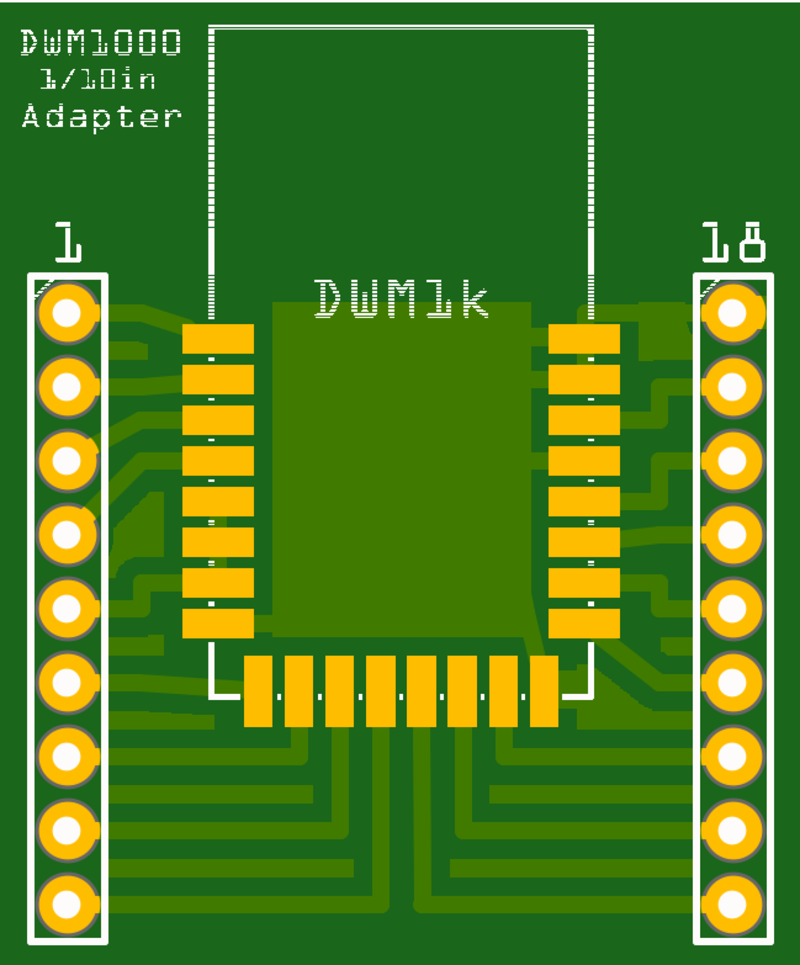
\includegraphics[width=0.28\textwidth]{pcb_dwm1000_adapterboard_top}
  \caption{\Gls{pcb}--Adapterboard für den \textit{DWM1000}.}
  \label{fig:pcb_dwm1000_adapterboard_top}
\end{figure}


\begin{comment}
------------------------------------------------------------------------------------------
+ Der initiale Aufbau erfolgt zu Evaluationszwecken auf einem Steckboard und zusätzlich auf einer separaten Lochstreifenplatine um das Zusammenspiel zweier UWB--Module zu testen. Nach dem erfolgreichen Systemtest wird aus dem erstellten Schaltplan, ein PCB--Layout erstellt, mehrere PCB--Boards bestellt und nach der Lieferung zusammengebaut und noch mal getestet.
+ Antenne
+ Aufrecht stehend
+ Batterie auf der Rückseite bietet stabilität
	+ Flachere Akkus können auch verwendet werden
+ Ansteckbares FTDI
+ Preis pro Platinengröße
- Footprint of DWM1000
+ AutoRoute
- TODO: Ground Fill with Copper
- Wikipedia: In der Antennentechnik (Satellitenfunk) bezeichnet der Azimutwinkel die horizontale Ausrichtung einer Antenne, im Gegensatz zur Elevation, die den vertikalen Winkel zwischen Horizont und Antennenrichtung angibt.
\end{comment}
\subsection{Platinendesign}

Nachdem die Korrektheit des Schaltplans durch die Prototypen bestätigt wurde, kann nun das Layout für die endgültigen \Gls{pcb}--Platinen erstellt werden. Sowohl der Schaltplan als auch das Platinen--Layout werden mit dem Programm \textit{fritzing}\cite{fritzing} erstellt. Jedes im Schaltplan verwendete elektrische Bauelement besitzt einen \Gls{footprint}, der die Größe des Bauelementes und seine elektrischen Anschlüsse auf der Leiterplatte festlegt, siehe \figurename~\ref{fig:breadboard_schematic_pcb}. Anhand des \Glspl{footprint} muss nun jedes Bauteil so platziert werden, das es idealerweise möglichst wenig Platz auf der Leiterplatte verschwendet wird. Den je kleiner die Leiterplatte ist, desto günstiger in der Herstellung.

\begin{figure}
	\begin{subfigure}[t]{0.3\textwidth}
		\centering
		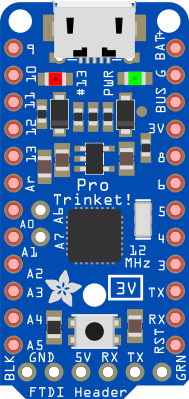
\includegraphics[width=0.5\textwidth]{pro_trinket_breadboard}
		\caption{Reales Bauelement}
		\label{fig:pro_trinket_breadboard}
	\end{subfigure}
	\quad
	\begin{subfigure}[t]{0.3\textwidth}
		\centering
		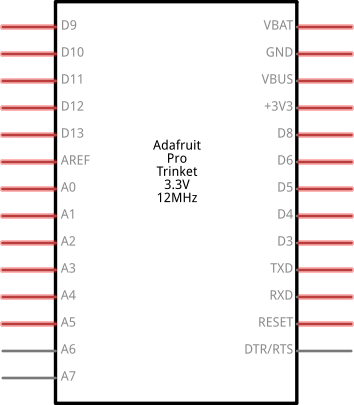
\includegraphics[width=\textwidth]{pro_trinket_schematic}
		\caption{Bauelement im Schaltplan}
		\label{fig:pro_trinket_schematic}
	\end{subfigure}
	\quad
	\begin{subfigure}[t]{0.3\textwidth}
		\centering
		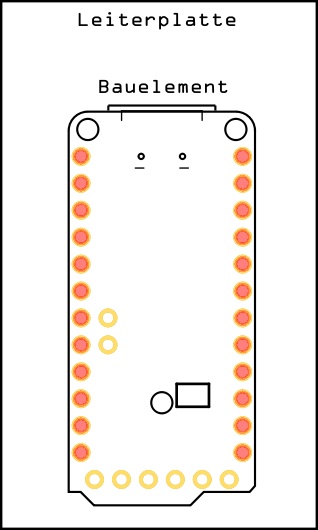
\includegraphics[width=\textwidth]{pro_trinket_pcb}
		\caption{Bauelement mit seinem \Gls{footprint} auf einer Leiterplatte.}
		\label{fig:pro_trinket_pcb}
	\end{subfigure}
	\caption{Designstufen eines elektrischen Bauelementes.}
	\label{fig:breadboard_schematic_pcb}
\end{figure}

Die Leiterplatte besitzt eine rechteckige Form, mit den Maßen \SI{43 x 75}{\mm}. Am höchsten Punkt der Leiterplatte befindet sich die Antenne des \Gls{uwbt}, dadurch wird gewährleistet das die Antenne in horizontaler Richtung ein gleichmäßiges Abstrahlmuster aufweist, siehe \figurename~\ref{fig:dwm1000_antenna_radiation_pattern}. Des Weiteren empfehlen die \textit{Application Board Layout Guidelines} das unterhalb der Antenne sich keine Metall oder andere nicht RF transparente Materialien befinden und ein freier horizontaler Abstand von mindestens \SI{10}{\mm} eingehalten wird, siehe \figurename~\ref{fig:dwm1000_application_board_keep_out_areas}.

Links neben dem \Gls{uwbt} befinden sich, gut sichtbar, die Status-Leuchtdioden. Unterhalb der Status-Leuchtdioden befindet sich der Ladeschaltkreis für den Lithium--Ion Akku sowie der Ein--Aus--Schalter. Auf der Rückseite der Leiterplatte wird der Lithium--Ion Akku befestigt. Dadurch ist ein aufrechter Stand des \Gls{uwbm} möglich. Die Leiterplatte ist mit \SI{75}{\mm} ca. \SI{10}{\mm} größer als der Lithium--Ion Akku, sodass es zu keiner Beeinträchtigung der Antenne kommt.

Im unteren rechten Bereich der Leiterplatte befindet sich der \textit{Pro Trinket}, also die Verarbeitungseinheit. Direkt daneben auf der linken Seite ist das optionale Datenübertragungsmodul vorgesehen. Da der \Gls{tag} auf dem Roboter in einer erhöhten Position befestigt wird, zeigt der \Gls{usb}--Stecker für das Datenübertragunsmodul in eine ideale Richtung.

Nachdem jedes elektrische Bauelement auf der Leiterplatte positioniert wurde, muss noch die Verdrahtung der einzelnen Bauelemente erfolgen. Sehr bequem erfolgt die Verdrahtung über die \textit{Autoroute}--Funktion. Hierbei errechnet ein Algorithmus, welchen Weg die Leiterbahnen nehmen sollen um alle notwendigen Pins miteinander zu Verbindungen ohne das sich ihre Wege überschneiden. Das fertige Layout der Leiterplatte ist in \figurename~\ref{fig:pcb_uwb_modul_board_top} abgebildet. In der \figurename~\ref{fig:uwb_modul} ist ein fertig aufgebautes \Gls{uwbm} abgebildet.

\begin{figure}
	\centering
	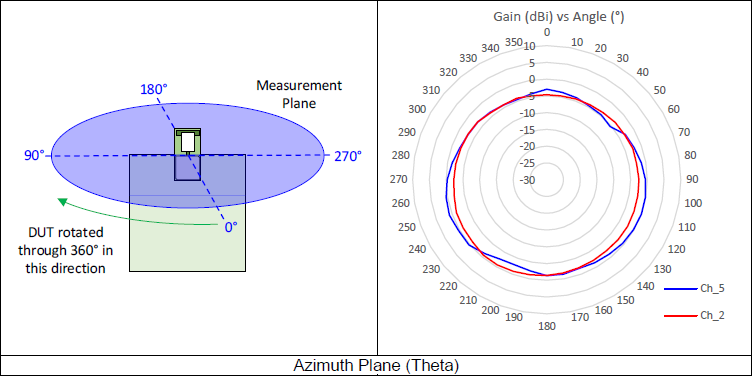
\includegraphics[width=\textwidth]{dwm1000_antenna_radiation_pattern}
	\caption{Das Antennenabstrahlmuster in horizontaler Richtung.}
	\label{fig:dwm1000_antenna_radiation_pattern}
	\source{\cite{decawave2016dwm1kdatasheet}}
\end{figure}
	
\begin{figure}
	\centering
	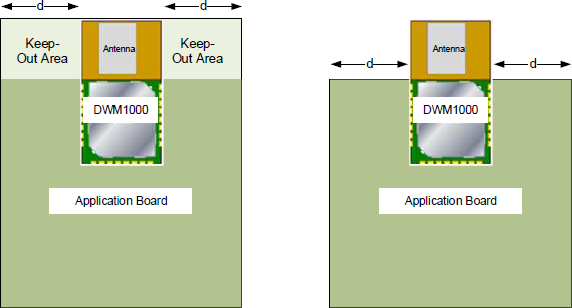
\includegraphics[width=\textwidth]{dwm1000_application_board_keep_out_areas}
	\caption{Antennenfreiräume}
	\label{fig:dwm1000_application_board_keep_out_areas}
	\source{\cite{decawave2016dwm1kdatasheet}}
\end{figure}

%\begin{figure}
%	\centering
%	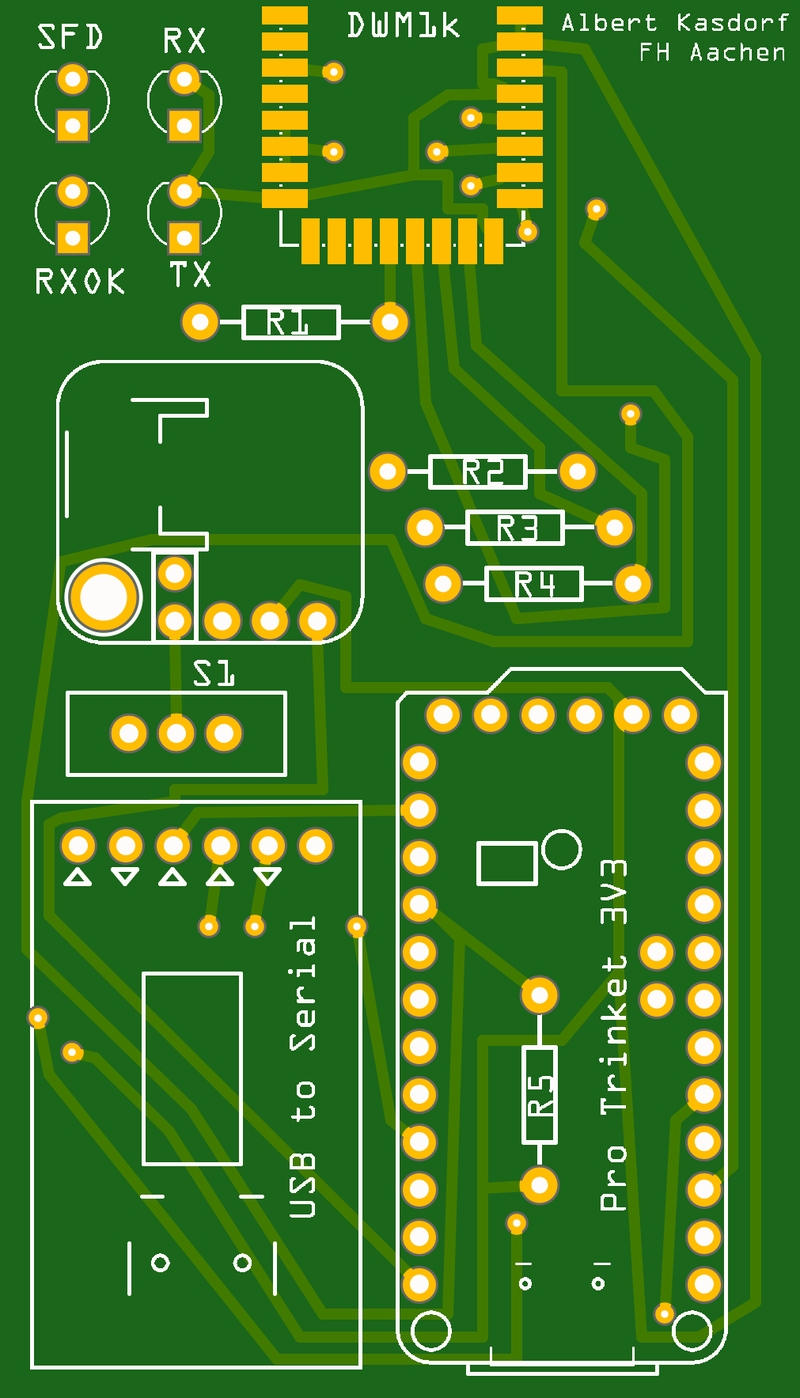
\includegraphics[width=0.25\textwidth]{pcb_uwb_modul_board_top}
%	\caption{Das fertige Leiterplatten Layout.}
%	\label{fig:pcb_uwb_modul_board_top}
%\end{figure}
%
%\begin{figure}
%	\centering
%	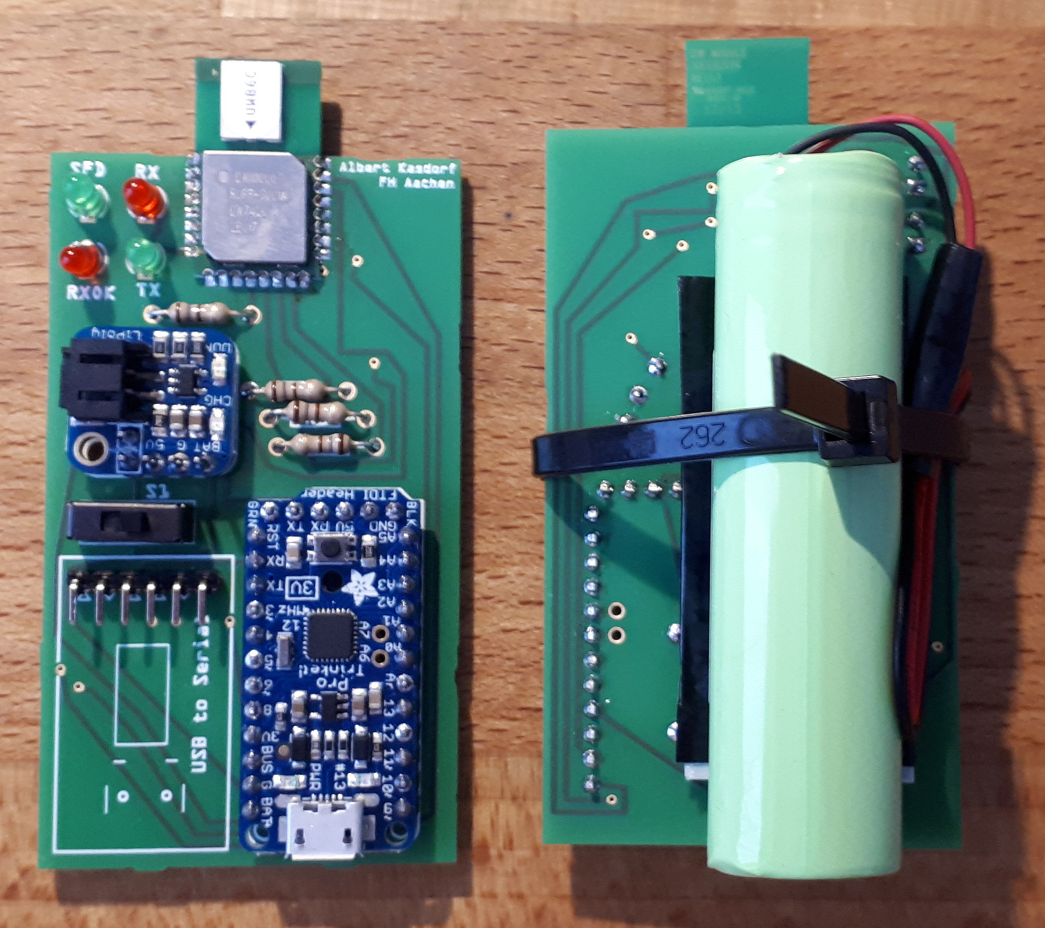
\includegraphics[width=0.5\textwidth]{uwb_modul}
%	\caption{Vorder- und Rückansicht eines \gls{uwbm}.}
%	\label{fig:uwb_modul}
%\end{figure}

\begin{figure}
	%\centering
	\begin{subfigure}[t]{0.3\textwidth}
		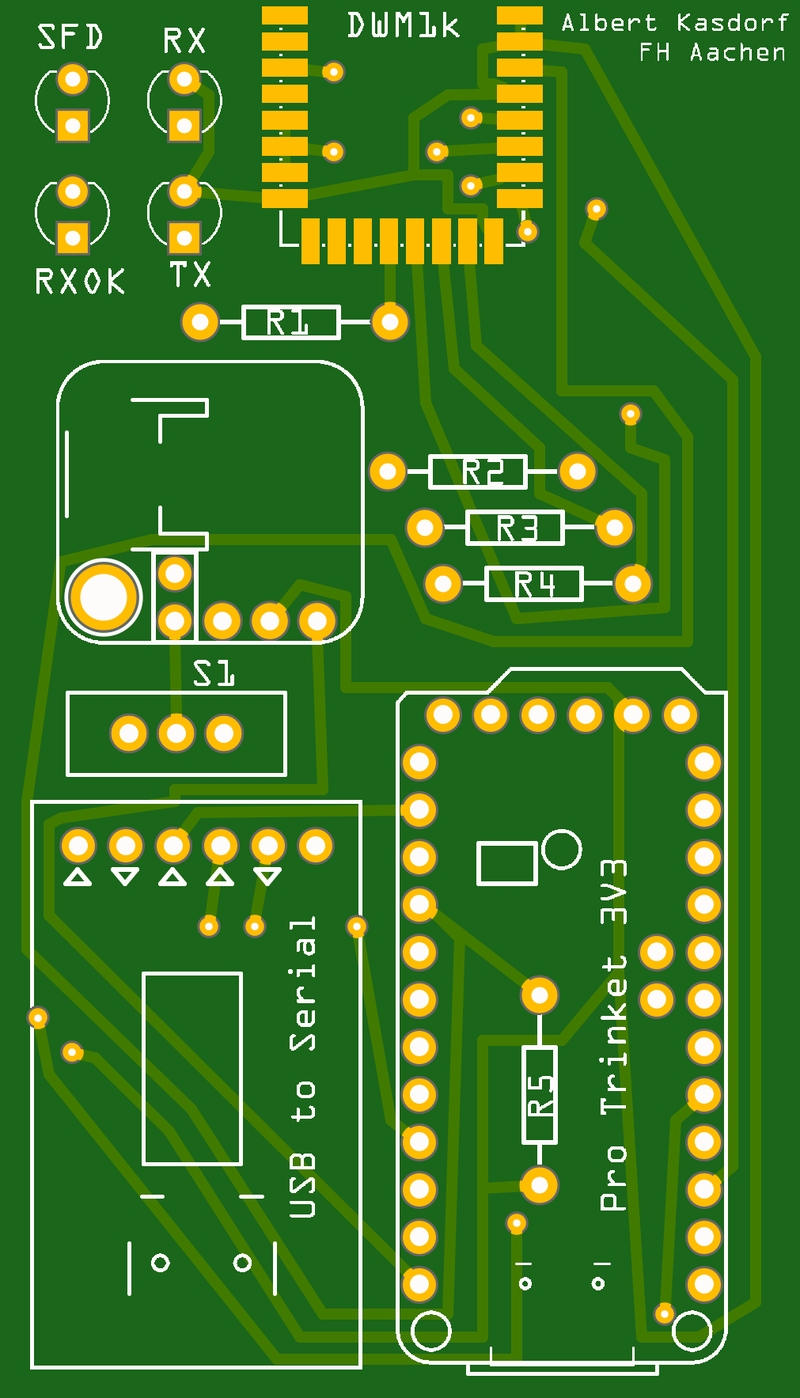
\includegraphics[width=\textwidth]{pcb_uwb_modul_board_top}
		\caption{Das fertige Leiterplatten Layout.}
		\label{fig:pcb_uwb_modul_board_top}
	\end{subfigure}
	\hfill
	\begin{subfigure}[t]{0.6\textwidth}
		\centering
		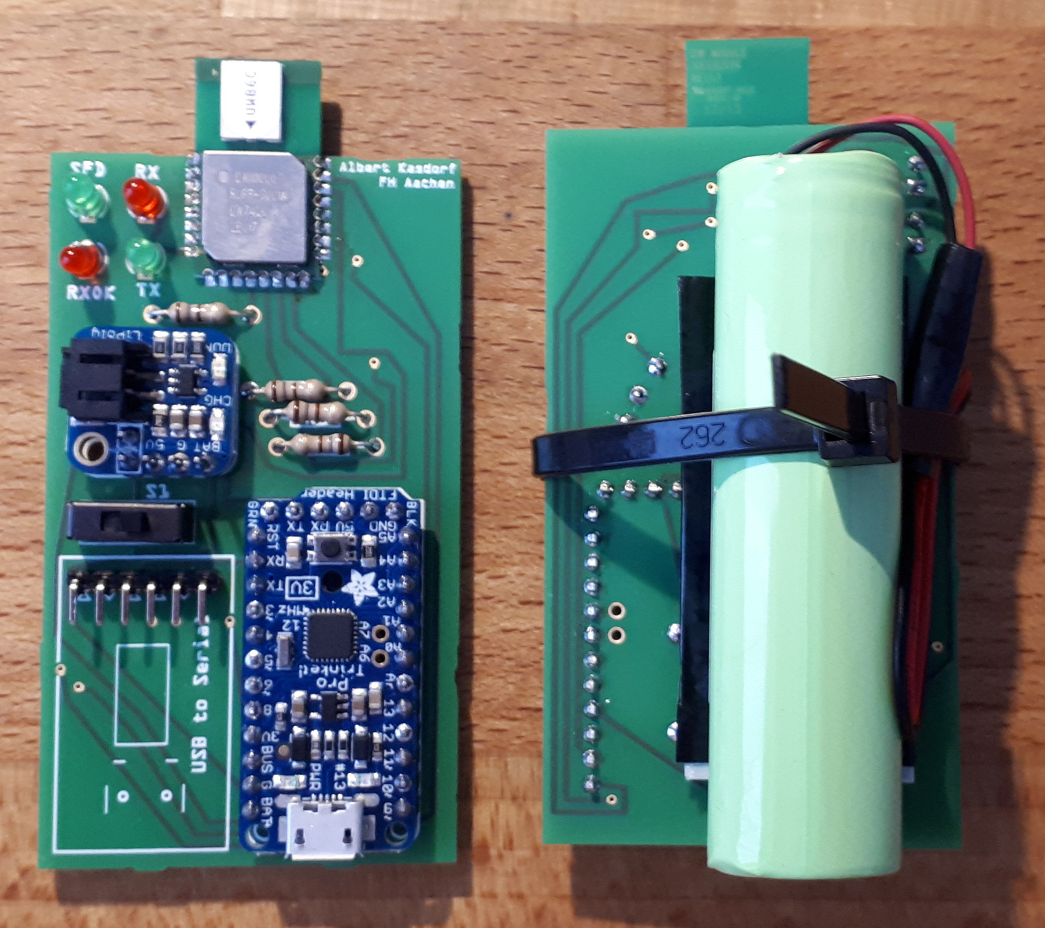
\includegraphics[width=\textwidth]{uwb_modul}
		\caption{Vorder- und Rückansicht eines \gls{uwbm}.}
		\label{fig:uwb_modul}
	\end{subfigure}
	\caption{Fertige \glspl{uwbm}.}
	\label{fig:fertige_uwb_module}
\end{figure}


\begin{comment}
------------------------------------------------------------------------------------------
- Woher kommt die Steuersoftware und wer ist für diese Zustandig?
	- Aktive Entwicklung wurde eingestellt
	- Was kann ich mit dieser Software machen?
\end{comment}
\subsection{Steuersoftware}

Als Basis für die Steuersoftware wurde das GitHub--Projekt \cite{Trojer2015} verwendet. Neben einer stabilen Basis für die Kommunikation mit dem \textit{DWM1000}, existiert eine Implementierung des \Gls{twr}--Verfahrens von \textit{DecaWave}. Die aktive Entwicklung ist mittlerweile eingestellt, es werden jedoch weiterhin \textit{Pull--Requests\footnotemark} für Fehlerkorrekturen und neue Funktionalitäten angenommen.

% https://blog.seibert-media.net/blog/2014/05/12/git-workflows-der-pull-request-workflow-teil-1/
\footnotetext{Ein Pull--Request dient dazu, eine Weiterentwicklung oder Fehlerkorrektur mit anderen Entwicklern zu diskutieren und dann auf einfach Weise in den Hauptentwicklungszweig zu integrieren.}


\begin{comment}
------------------------------------------------------------------------------------------
- Klassendiagramme der wichtigsten Elemente
	- Auswelchen wichtigen Elementen besteht diese Bibliothek?
	- DW1000
	- DW1000Time
	- DW1000Device
	- DW1000Ranging
- Die Steuersoftware besteht aus den Klassen \textit{DW1000}, \textit{DW1000Time}, \textit{DW1000Ranging}, \textit{DW1000Device} die im folgenden Beschrieben werden.
\end{comment}
\subsubsection{Klassenübersicht}

Die Klasse \textit{DW1000} enthält alle Basisfunktionalität um mit dem \textit{DWM1000} arbeiten zu können. Dazu gehören die Kommunikation über den \Gls{spi}--Bus, das Lesen und Schreiben der Konfiguration und das Erstellen und Empfangen von Nachrichten. Über einen Low--Level Zugriff ist es zusätzlich möglich auf Funktionalitäten des \textit{DW1000} zuzugreifen die in dem ursprünglichen Klassendesign nicht vorgesehen waren.

Zeitstempel spielen beim Nachrichtenaustausch und bei der Entfernungsmessung eine zentrale Rolle. Jedoch werden die Zeitstempel als \SI{40}{\bit} Zahl gespeichert. Um die Verwendung zu erleichtern und Fehlerquellen auszuschließen wurde die Hilfsklasse \textit{DW1000Time} bereitgestellt.

Über die Klasse \textit{DW1000Ranging} ist eine Implementierung des \Gls{twr}--Verfahrens von \textit{DecaWave} verfügbar, siehe Abschnitt~\ref{subsec:double_sided_two_way_ranging}. Mittels drei Rückruffunktionen (engl. Callback function) teilt die Klasse dem Anwender mit, welche Entfernungen gemessen wurde und ob neue Quellen für Entfernungsmessungen hinzugekommen oder verschwunden sind. Jede Quelle für eine Entfernungsmessung wird mit der Klasse \textit{DW1000Device} modelliert. Neben der gemessenen Entfernung beinhaltet die Klasse auch eine eindeutige Identifikationsnummer. 


\begin{comment}
------------------------------------------------------------------------------------------
- Basisscript
	- Wie sieht ein ganz triviales Beispiel aus?
	- Wie ist der Programmablauf des Beispiels?
	- Für das DW1000Ranging
	- Wie kann man Daten austauschen? JSON
- Datenaustausch zwischen Host und µC
- ArduinoJson Assistant
	- https://arduinojson.org/assistant/
\end{comment}
\subsubsection{Datenaustausch}

Der erste Bereich des Datenaustausches findet zwischen den \Glsuseri{uwbm} statt. Hierfür wird mindestens ein \Gls{anchor} und \Gls{tag} benötigt. In der \autoref{lst:uwb_modul_as_anchor} ist der Quellcode eines \Gls{anchor} abgebildet.
Über die ersten zwei Zeile wird die \textit{\Gls{spi}--} und \textit{DW1000Ranging}--Bibliothek in das Programm eingebunden.
Um eine Kommunikation mit dem \textit{DWM1000} aufzubauen muss der Methode \textit{initCommunication} die Belegung des \textit{Reset--}, \textit{\Gls{ss}--} und \textit{\Gls{irq}--Pin} übergeben werden.
Nach dem Aufruf der Methode \textit{startAsAnchor} fungiert das \Gls{uwbm} als \Gls{anchor}. Die notwendigen Parameter sind dabei die eindeutige Adresse, der Messmodus und ob eine zufällige Geräteadresse generiert werden soll. Wenn der letzte Parameter \textit{false} ist, werden aus den ersten zwei Bytes der eindeutigen Adresse, die Geräteadresse gebildet. Der zyklische Aufruf der Methode \textit{loop} sorgt für die Nachrichtenverarbeitung des \Glsuserii{uwbm}.

\begin{listing}
	\begin{minted}{cpp}
#include <SPI.h>
#include <DW1000Ranging.h>

void setup() {
  Serial.begin(115200);

  DW1000Ranging.initCommunication(9, SS, 3);
  
  DW1000Ranging.startAsAnchor("B1:00:00:00:B1:6B:00:B5", DW1000.MODE_LONGDATA_RANGE_ACCURACY, false);
}

void loop() { DW1000Ranging.loop(); }
	\end{minted}
	\unskip
	\caption{Quellcode für ein \Gls{uwbm} das als \Gls{anchor} konfiguriert ist.}
	\label{lst:uwb_modul_as_anchor}
\end{listing}

Das Gegenstück zum \Gls{anchor} ist in der \autoref{lst:uwb_modul_as_tag} abgebildet. Jede gemessene Entfernung zwischen dem \Gls{tag} und einem \Gls{anchor} soll per \Gls{usb} an den Computer übertragen werden. Der Datenaustausch erfolgt dabei im \Gls{json}--Format, daher wird die Bibliothek \textit{ArduinoJson} benötigt.
Da dieses \Gls{uwbm} als \Gls{tag} fungieren soll, muss anstatt \textit{startAsAnchor} die Methode \textit{startAsTag} aufgerufen werden. Die Bedeutung der Parameter zwischen den beiden Methoden bleibt identisch.
Neu ist der Aufruf der Methode \textit{attachNewRange}, \textit{attachNewDevice} und \textit{attachInactiveDevice}. Jeder der Methoden wird die Adresse einer Rückruffunktion übergeben. Diese Funktionen werden immer dann aufgerufen, wenn eine neue Entfernungen gemessen wurde und wenn eine neue Quelle für die Entfernungsmessungen hinzugekommen oder verschwunden ist.
Alle Rückruffunktionen rufen ihrerseits die Funktion \textit{transmitDATA} auf. In dieser wird mittels der Klasse \textit{StaticJsonBuffer} ein \textit{JsonObject} erstellt, mit Daten im Schlüssel--Wert--Format (engl. Key--Value) belegt und dann mittels der Methode \textit{printTo(Serial)} über die \Gls{usb}--Schnittstelle an den Computer versendet. Das Format der Daten ist in der \autoref{lst:data_in_json_format} abgebildet.

\begin{listing}
	\begin{minted}{cpp}
#include <SPI.h>
#include <DW1000Ranging.h>
#include <ArduinoJson.h>

enum class Events : byte {
  NEW_RANGE=0, NEW_DEVICE=1, INACTIVE_DEVICE=2
};

void setup() {
  Serial.begin(115200);
  
  DW1000Ranging.initCommunication(9, SS, 3);
  DW1000Ranging.attachNewRange(newRange);
  DW1000Ranging.attachNewDevice(newDevice);
  DW1000Ranging.attachInactiveDevice(inactiveDevice);

  DW1000Ranging.startAsTag("A0:00:00:00:B1:6B:00:B5", DW1000.MODE_LONGDATA_RANGE_ACCURACY, false);
}

void loop() {
  DW1000Ranging.loop();
}

void newRange() {
  transmitDATA(Events::NEW_RANGE, DW1000Ranging.getDistantDevice());
}

void newDevice(DW1000Device* device) {
  transmitDATA(Events::NEW_DEVICE, device);
}

void inactiveDevice(DW1000Device* device) {
  transmitDATA(Events::INACTIVE_DEVICE, device);
}

void transmitDATA(const Events event, const DW1000Device* device) {
  StaticJsonBuffer<200> jsonBuffer;
  JsonObject& root = jsonBuffer.createObject();

  root["type"] = static_cast<byte>(event);
  root["aa"] = device->getShortAddress();
  root["r"] = (event==Events::NEW_RANGE) ? device->getRange() : 0.0f;
  
  root.printTo(Serial);
  Serial.println();
}
	\end{minted}
	\unskip
	\caption{Quellcode für ein \Gls{uwbm} das als \Gls{tag} konfiguriert ist.}
	\label{lst:uwb_modul_as_tag}
\end{listing}


\begin{listing}
	\begin{minted}{json}
{"type": 0, "aa": 160, "r": 1.01}
	\end{minted}
	\unskip
	\caption{Datenzeile im \Gls{json}--Format beim Austausch zwischen \Gls{uwbm} und Computer.}
	\label{lst:data_in_json_format}
\end{listing}

Nach dem die Daten an den Computer gesendet wurde, müssen diese entgegengenommen und in das \Gls{ros}--System eingespeist werden. Dies geschieht über die \autoref{lst:json_to_ros}.
Zuerst wird das \Gls{ros}--System über \textit{rospy.init\_node} initalisiert. Um Nachrichten versendet zu können, wird zusätzlich ein \textit{Publisher} benötigt. Dieser wird über den Aufruf von \textit{rospy.Publisher} erstellt. Die Verbindung zu dem \Gls{uwbm} wird über den Aufruf \textit{serial.Serial} hergestellt.
Mittels der \Gls{ros}--Nachricht \textit{ObservationRangeBeacon} wird die Sensor--Charakteristik des \Glsuserii{uwbm} beschrieben. Hierzu gehören die minimal und maximal messbare Entfernung, das Sensorrauschen, eine oder mehrere Entfernungsmessungen und einige \Gls{ros} spezifische Angaben wie z.B. das Koordinatensystem in dem sich das \Gls{uwbm} befindet.
Danach werden solange Daten von dem \Gls{uwbm} gelesen bis der \Gls{ros}--Knoten beendet wird. Jeder gelesen Datensatz wird mittels der Methode \textit{json.loads(line)} untersucht, in ein \Gls{json}--Objekt konvertiert, und im Fehlerfall übersprungen. Gültige Entfernungsdaten werden in den Attributen \textit{range} und \textit{id} des Feldes \textit{orb.sensed\_data} gespeichert.
Der Aufruf \textit{pub.publish(orb)} übergibt die zuvor erstellte Nachricht an das \Gls{ros}--System.

\begin{listing}
	\begin{minted}{python}
import json
import rospy
import serial

from mrpt_msgs.msg import ObservationRangeBeacon
from mrpt_msgs.msg import SingleRangeBeaconObservation

def main():
  rospy.init_node('beacon_publisher')
  pub = rospy.Publisher('/beacon', ObservationRangeBeacon, queue_size=10)
  ser = serial.Serial('/dev/CP2104_Friend', 115200, timeout=2)

  orb = ObservationRangeBeacon()
  orb.header.frame_id = 'uwb_reciever_link'
  orb.min_sensor_distance = 0.0
  orb.max_sensor_distance = 120.0
  orb.sensor_std_range = 0.1
  orb.sensed_data.append(SingleRangeBeaconObservation())

  while not rospy.is_shutdown():
    line = ser.readline()
    try:
      obj = json.loads(line)
    except ValueError:
      continue

    orb.header.stamp = rospy.Time.now()
    orb.header.seq = orb.header.seq + 1
    orb.sensed_data[0].range = obj["r"]
    orb.sensed_data[0].id = obj["aa"]

    pub.publish(orb)
	\end{minted}
	\unskip
	\caption{Quellcode um eine Entfernungsmessung an das \Gls{ros}--System zu übergeben.}
	\label{lst:json_to_ros}
\end{listing}

Der vollständige Quellcode mit Kommentaren und Fehlerbehandlung kann in dem GitHub--Projekt \cite{kasdorf2017roslamwithuwb} eingesehen werden.


\begin{comment}
--------------------------------------------------------------------------------
\end{comment}
\subsection{Kalibrierung [new]}

Je genauer sich die Zeitstempel für den Empfang bzw. für das Versenden einer Nachricht bestimmen lassen, desto genauer ist auch die gemessene Entfernung. Idealerweise entsprich die Differenz zwischen zwei Zeitstempeln der \Gls{tof}. In der Realität ist die Differenz jedoch deutlich größer. Als eine der Ursachen kann die herstellungsbedinge Ungenauigkeiten in den verwendeten Komponenten in Betracht gezogen werden, genauer gesagt geht es um die Antennenverzögerung. Unter der Antennenverzögerung versteht man die Zeitspanne die die Antenne benötigt um mit der Übertragung der Nachricht zu starten bzw. um eine Nachricht zu empfangen, siehe  \autoref{fig:decawave2014calibration_fig1}.

\begin{figure}[h]
	\centering
	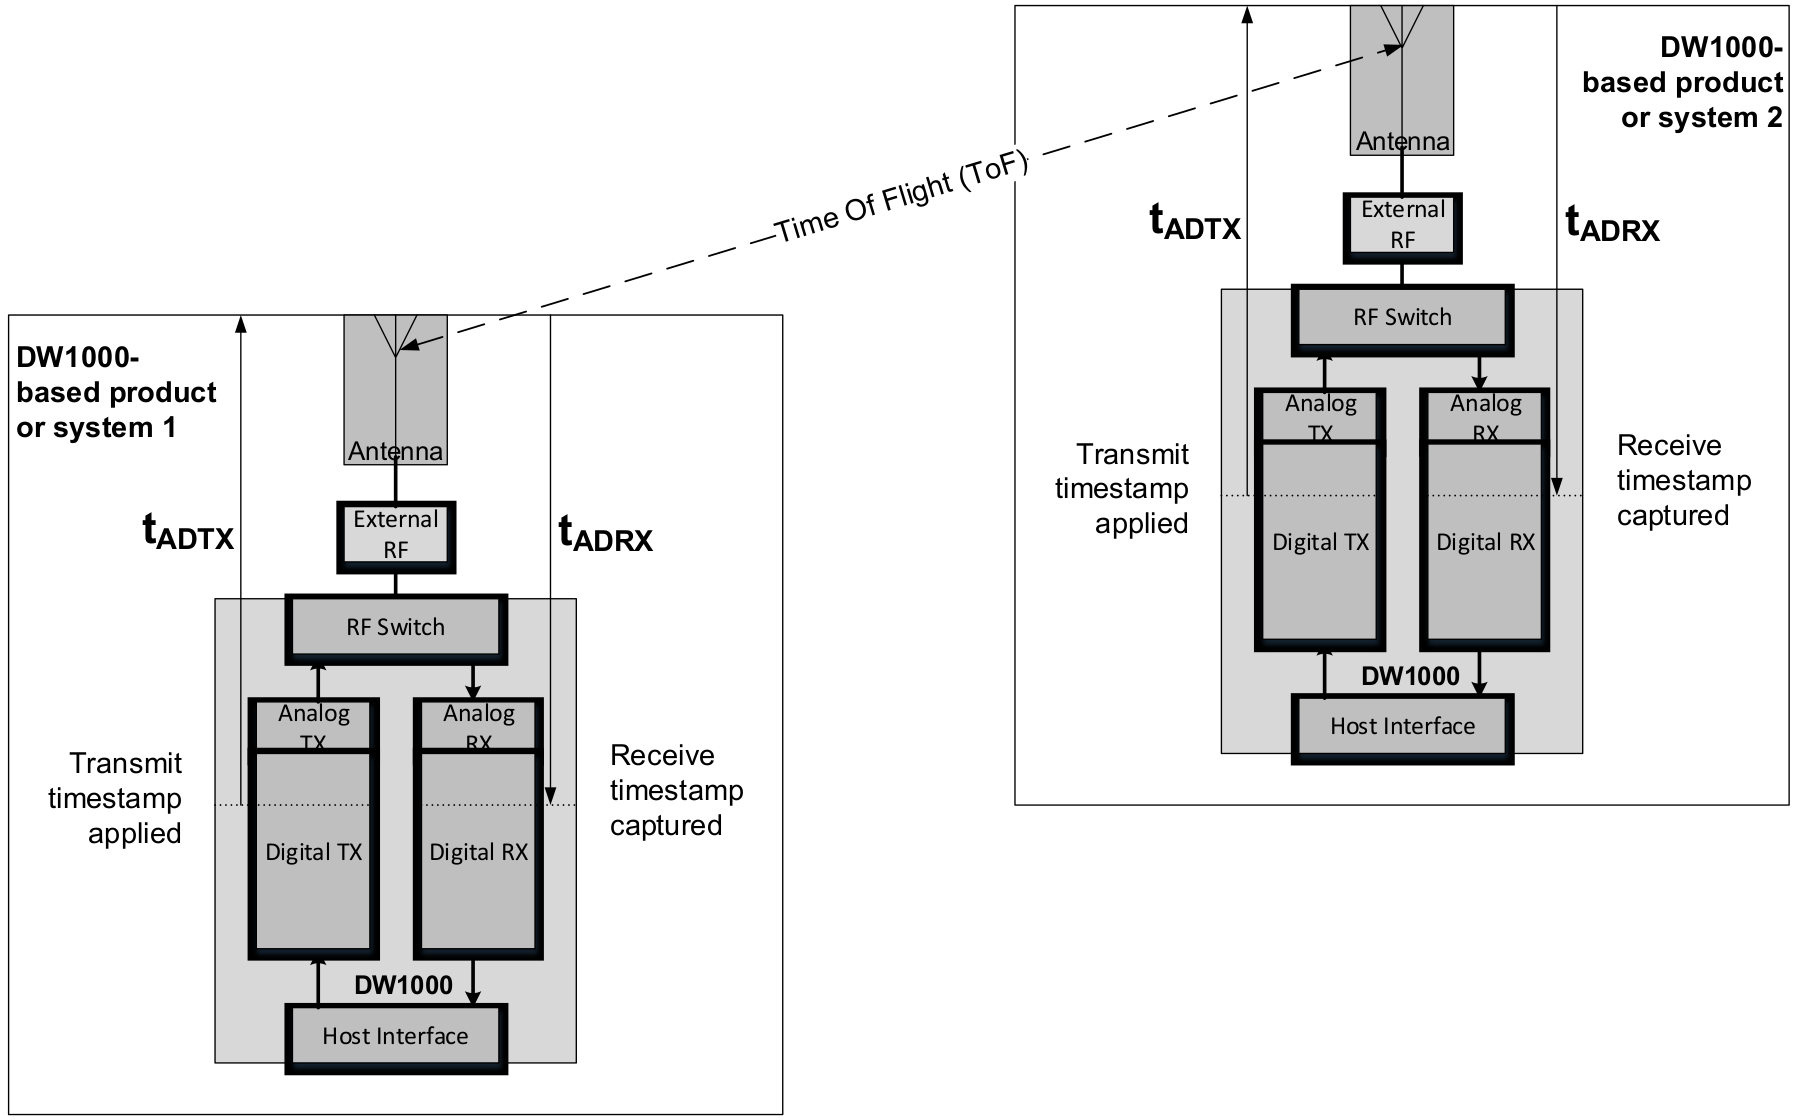
\includegraphics[width=0.9\linewidth]{decawave2014calibration_fig1}
	\caption{Antennenverzögerung zwischen zwei \Glsuseri{uwbm}.}
	\label{fig:decawave2014calibration_fig1}
	\source{\cite{decawave2014calibration}}
\end{figure}

Die gemessene Zeitspanne ergibt sich dabei aus der Gleichung: 

\begin{equation}
tof_{measured}=t_{ADTX}+tof_{actual}+t_{ADRX}\label{eq:antenna_delay_1}
\end{equation}

wobei der Term $t_{ADTX}$ die Antennenverzögerung für das Versenden und $t_{ADRX}$ für das Empfangen auf den gegenüberliegenden \Glsuseri{uwbm} beschreibt. Es wird davon ausgegangen, dass die Antennenverzögerung für das Senden und Empfangen auf einem \Gls{uwbm} gleich lang ist. \cite{decawave2016dw1kusermanual}

Um die Antennenverzögerung zu bestimmen, wird diese initial auf null eingestellt, die \Gls{uwbm} in einem bekannten Abstand positioniert und dann von jedem \Gls{uwbm} eine Reihe von Messungen aufgezeichnet. In den nachfolgenden Abschnitten werden zwei Verfahren vorgestellt, mit der sich die Antennenverzögerungen aus den aufgezeichneten Messungen bestimmen lässt.


\begin{comment}
--------------------------------------------------------------------------------
\end{comment}
\subsubsection{DecaWave [new]}

Um die Antennenverzögerung pro \Gls{uwbm} zu bestimmen, wird von \textit{DecaWave} ein genetischer Algorithmus vorgeschlagen. \cite{decawave2014calibration}

Im ersten Schritt wird eine initiale Kandidatenliste mit eintausend Kandidaten erstellt. Jeder Kandidat beinhaltet für jedes \Gls{uwbm} eine Antennenverzögerungen. Die Werte sind dabei gleichmäßig um den Wert \SI{513}{\ns} mit einer Streuung von \SI{6}{\ns} verteilt.

Im nächsten Schritt wird für jeden Kandidaten seine spezifische \Gls{tof}--Zeit berechnet, siehe \autoref{eq:decawave_ad1}.

\begin{equation}
tof_{candidate}=\frac12 del_{chip1} + \frac12 del_{chip2} + tof_{measured}\label{eq:decawave_ad1}
\end{equation}

Bei $tof_{measured}$ handelt es sich um eine $n \times n$ Matrix mit den gemessenen \Gls{tof}--Zeiten zwischen den \Glsuseri{uwbm}, siehe \autoref{eq:decawave_tof_measured}.

\begin{equation}
tof_{measured} = \begin{pmatrix}0 & tof_{m12} & tof_{m13} \\ tof_{m21} & 0 & tof_{m23} \\ tof_{m31} & tof_{m32} & 0 \end{pmatrix} \label{eq:decawave_tof_measured}
\end{equation}

Die Matrix $del_{chip1}$ enthält pro Spalte die Antennenverzögerung eines \Glsuserii{uwbm} und die diagonalen Element sind alle null. Bei der Matrix $del_{chip2}$ handelt es sich um die transponierte Matrix von $del_{chip1}$, siehe \autoref{eq:decawave_del_chip}.

\begin{equation}
Del_{chip1} = \begin{pmatrix}0 & t_{ad2} & t_{ad3} \\ t_{ad1} & 0 & t_{ad3} \\ t_{ad1} & t_{ad2} & 0 \end{pmatrix}; \qquad Del_{chip2} = \begin{pmatrix}0 & t_{ad1} & t_{ad1} \\ t_{ad2} & 0 & t_{ad2} \\ t_{ad3} & t_{ad3} & 0 \end{pmatrix} \label{eq:decawave_del_chip}
\end{equation}

Die Bewertung eines Kandidaten findet dabei über die Berechnung der Norm aus der Differenz zwischen der tatsächlichen \Gls{tof}--Zeit und \Gls{tof}--Zeit des Kandidaten statt, siehe \autoref{eq:decawave_ad2}. Je kleiner die Norm desto besser die Bewertung des Kandidaten.

\begin{equation}
rank_{candidate}=\lVert (tof_{actual} - tof_{candidate}) \lVert\label{eq:decawave_ad2}
\end{equation}

Nach dem alle Kandidaten bewertet worden sind, werden die besten \SI{25}{\percent} weiterverwendet und die Restlichen verworfen. Um die Kandidatenliste nicht mit jeder Iteration kleiner werden zu lassen, werden aus den verbliebenden Kandidaten drei neue Gruppen mit einer alle zwanzig Iterationen abnehmenden Streuung erstellt.

Der Vorgang der Erstellung und Bewertung einer Kandidatenliste wird hundert Mal durchgeführt und sollte sich zum Ende hin der tatsächlichen Antennenverzögerung annähern.


\begin{comment}
--------------------------------------------------------------------------------
\end{comment}
\subsubsection{Lineares Gleichungssystem [new]}

Bei zwei \Glsuseri{uwbm} kann die \autoref{eq:antenna_delay_1} zwei Mal aufgestellt werden, für jede Richtung einmal. Bei drei \Glsuseri{uwbm} bereits sechs Mal. Allgemein gilt für die Anzahl der Gleichung die Formel $n(n-1)$. Damit lässt sich ein lineares Gleichungssystem aufstellen und somit die Antennenverzögerung pro \Gls{uwbm} berechnen.

Hierfür werden alle unbekannten Terme auf die linke Seite gebracht und alle bekannten auf die rechte Seite, siehe \autoref{eq:antenna_delay_2}.

\begin{equation}
t_{ad1} + t_{ad2} = tof_{measured} - tof_{actual} \label{eq:antenna_delay_2}
\end{equation}

Danach werden alle Gleichung in die Matrixform $A\cdot x=b$ gebracht und mit einem beliebigen Lösungsverfahren gelöst, siehe \autoref{eq:antenna_delay_3} für drei \Glspl{uwbm}. Die Koeffizientenmatrix enthält hierbei pro Zeile immer nur zwei Einsen, da für jede Entfernungsmessung nur zwei Antennenverzögerungen berücksichtigt werden.

\begin{equation}
\begin{pmatrix} 1 & 1 & 0 \\ 1 & 0 & 1 \\ 0 & 1 & 1 \end{pmatrix} \cdot \begin{pmatrix} t_{ad1} \\ t_{ad2} \\ t_{ad3} \end{pmatrix} = \begin{pmatrix} tof_{measured1} - tof_{actual1} \\ tof_{measured2} - tof_{actual2} \\ tof_{measured3} - tof_{actual3} \end{pmatrix} \label{eq:antenna_delay_3}
\end{equation}


	%%%%%%%%%%%%%%%%%%%%%%%%%%%%%%%%%%%%%%%%%%%%%%%%%%%%%%%%%%%%%%%%%%%%%%%%%%%%%%%%
%
%
%
%%%%%%%%%%
\chapter{Umsetzung des RO-SLAM in ROS}
\label{ch:ro_slam}

Im vorherigen Kapitel wurden mehrere \gls{uwbm} erstellt, darunter befand sich ein \gls{tag} und vier \gls{anchor}. Um die Entfernungen messen zu können, muss der \gls{tag} auf einer Roboterplattform montiert und die \gls{anchor} im Messbereich verteilt werden. Damit ist aber nur ein Teil der Hardwareanforderungen erfüllt. Es wird noch eine Roboterplattform benötigt, die zum einen um den \gls{tag} erweitert werden kann und zum anderen über ausreichend Leistungsreserven verfügt um alle \glspl{rosm} ausführen zu können, die für einen \gls{roslam} benötigt werden. Die Zusammenstellung dieser Roboterplattform ist bestandteil dieses Kapitel.

Die eingesetze Hardware bildet einen soliden Sockel für die Ausführung der \glspl{rosm}. Erweitert werden muss dieser noch um die Softwareseite. Mit der Übersicht über die Softwarearchitektur lässt sich eine grobe Vorstellung der eingesetzten \glspl{rosm} vermitteln. Einen tieferen Einblick in die \glspl{rosm} liefern die Abschnitte mit den \gls{ros} Hauptmodulen und -Nebenmodulen. Bei dem ersteren geht es um die Kernmodule die eine direkte bzw. indirekte Voraussetzung für den \gls{roslam} sind. Im letzteren werden die Module behandeln die notwendigen sind um zusätzliche Daten, Kennzahlen und Grafiken für die Auswertung zu extrahieren.

Nach dem die Hardware- und Softwarevoraussetzungen für den \gls{roslam} Algorithmus erfüllt wurden, wird ein Blick auf die Umsetzung des \gls{roslam} in dem \gls{mrpt} Framework geworfen.


%%%%%%%%%%%%%%%%%%%%%%%%%%%%%%%%%%%%%%%%%%%%%%%%%%%%%%%%%%%%%%%%%%%%%%%%%%%%%%%%
%
%	- Einsatz mobiler Roboter in der Logistik am Beispiel des Robotino
%		- http://www.r-moehrle.de/wissenschaftlicheArbeiten/robotino1.pdf
%
%%%%%%%%%%
\section{Roboterplattform}

Um die Messungen für den \Gls{roslam} aufzuzeichnen wird eine Roboterplattform benötigt, auf der das \Gls{uwbm} montiert werden kann. Zusätzlich wird noch eine Reihe weiterer Sensoren benötigt, die im Folgenden vorgestellt werden.

Also Roboterplattform dient dabei der Robotino 2 von Festo Didactic. Er gehört zur Klasse der holonomen Roboter, d.h. seinen Bewegungsmöglichkeiten unterliegen keinerlei Einschränkungen im zweidimensionalen Raum. Ermöglicht wird das, durch drei voneinander unabhängig arbeitenden omnidirektionalen Antriebseinheiten. Jede der drei Antriebseinheiten verfügt über einen Inkrementalgeber, mit dessen Hilfe abgeschätz wird, wie weit der Robotino gefahren ist. Um den Fehler der Inkrementalgeber in Kurvenfahrten zu reduzieren wird das digitale Gyroskop\footnotemark{} von Microinfinity eingesetzt. Gesteuert wird der Robotino über eine \SI{300}{\MHz} starke Verarbeitungseinheit auf Basis eines Linux Betriebssystems mit einem Echtzeitkernel. \cite{festo2007robotinomanual} \footnotetext{Model: CruizCore XG1000 / XG1010}

An der höchsten Position des Robotinos befindet sich ein 2D-Laser-Entfernungsmesser\footnotemark{} der Firma Sick. Mit einem Öffnungswinkel von \SI{270}{\degree} und einem Arbeitsbereich von \SIrange{0.05}{25}{\meter} ist es möglich, genaue Belegtheitskarten der Umwelt zu erstellen. \cite{sick2016operatingmanual} \footnotetext{Model: TiM571-2050101}

Die Verarbeitungseinheit des Robotinos ist leistungsfähig genug um die anstehenden Steuerungsaufgaben zu erfüllen. Jedoch ist diese von leistungshungrigen Anwendungen wie dem \Gls{roslam} überfordert. Aus diesem Grund wird eine zusätzliche Verarbeitungseinheit\footnote{Model: NUC5i7RYH} mit einem Intel Core i7\footnote{5. Generation des Intel Core i7-5557U Prozessor mit bis zu \SI{3.4}{\GHz}. \cite{intel2015nucproductbrief}} verwendet.

Die Fahrbefehle werden dem Robotino über einen Xbox Wireless Controller übermittelt.

\begin{figure}
	\centering
	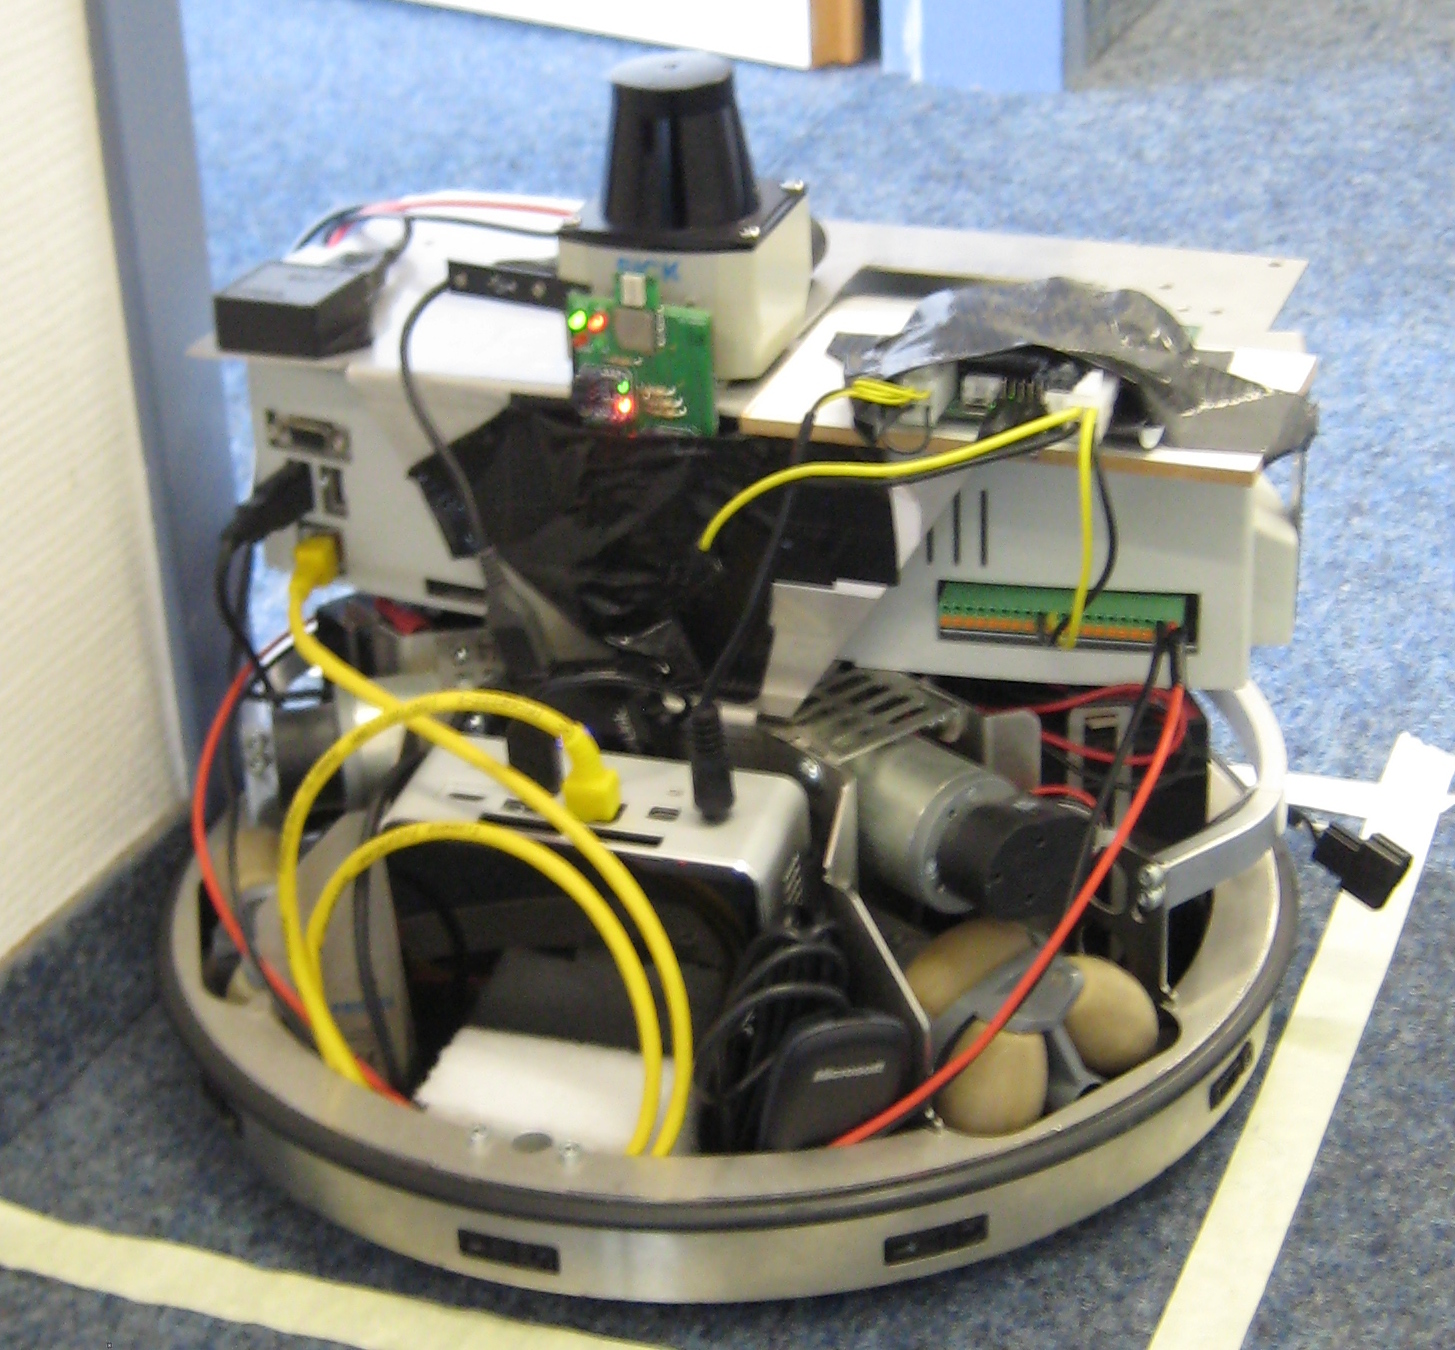
\includegraphics[width=0.5\textwidth]{robotino_front3}
	\caption{Die Frontansicht der fertig aufgebauten Roboterplattform.}
	\label{fig:robotino_front}
\end{figure}


%%%%%%%%%%%%%%%%%%%%%%%%%%%%%%%%%%%%%%%%%%%%%%%%%%%%%%%%%%%%%%%%%%%%%%%%%%%%%%%%
%
%	- Kurzbeschreibung der Modulfunktion
%	- Welche Funktion erfüllt dieses Modul
%	- Welche ROS-Messages/-Topics/-Services bietet dieses Modul
%
%%%%%%%%%%
\section{Softwarearchitektur}

Der Softwarearchitektur, siehe \autoref{fig:architektur_grouped}, lassen sich zwei Nachrichtentypen entnehmen die für den \gls{roslam} essentiell sind. Zum einen sind das die Daten der Entfernungsmessungen (mrpt\_msgs/ObservationRangeBeacon) zwischen den \gls{uwbm} und dem Transformationsbaum (tf2\_msgs/TFMessage) auf der anderen. Die Nachrichten des Transformationsbaums werden dabei nur indirekt benötigt, um zu bestimmen wie weit sich die Roboterplattform bewegt hat, sprich die Odometrieinformationen.

Als Datenquelle für den Transformationsbaum sind zuerst die statischen Transformationen zu nennen, dann die Belegtheitskarten für die Transformation von dem Odometrie- in das Kartenkoordinatensystem und zuletzt die zwei Arten der Odometrie. Die erste liefert die Daten anhand der Inkrementalgeber in der Antriebseinheit und die zweite eine Odometrie über das auswerten der 2D-Laser-Entfernungsmessers. Bei der Laser-Odometrie haben sich zwei unterschiedliche Verfahren etabliert und alle drei Verfahren sollen auf ihre Genauigkeit Untersucht werden.

Der untere Bereich, in der \autoref{fig:architektur_grouped}, ist über keinen Datenbus mit den anderen \gls{rosm} verbunden. Jedoch wird dieser zum einen benötigt um die Kommunikation zwischen der Robotino Steuereinheit herzustellen und zum anderem um die Roboterplattform als Ganzes durch ein Eingabegerät zu steuern.

\begin{figure}
	\centering
	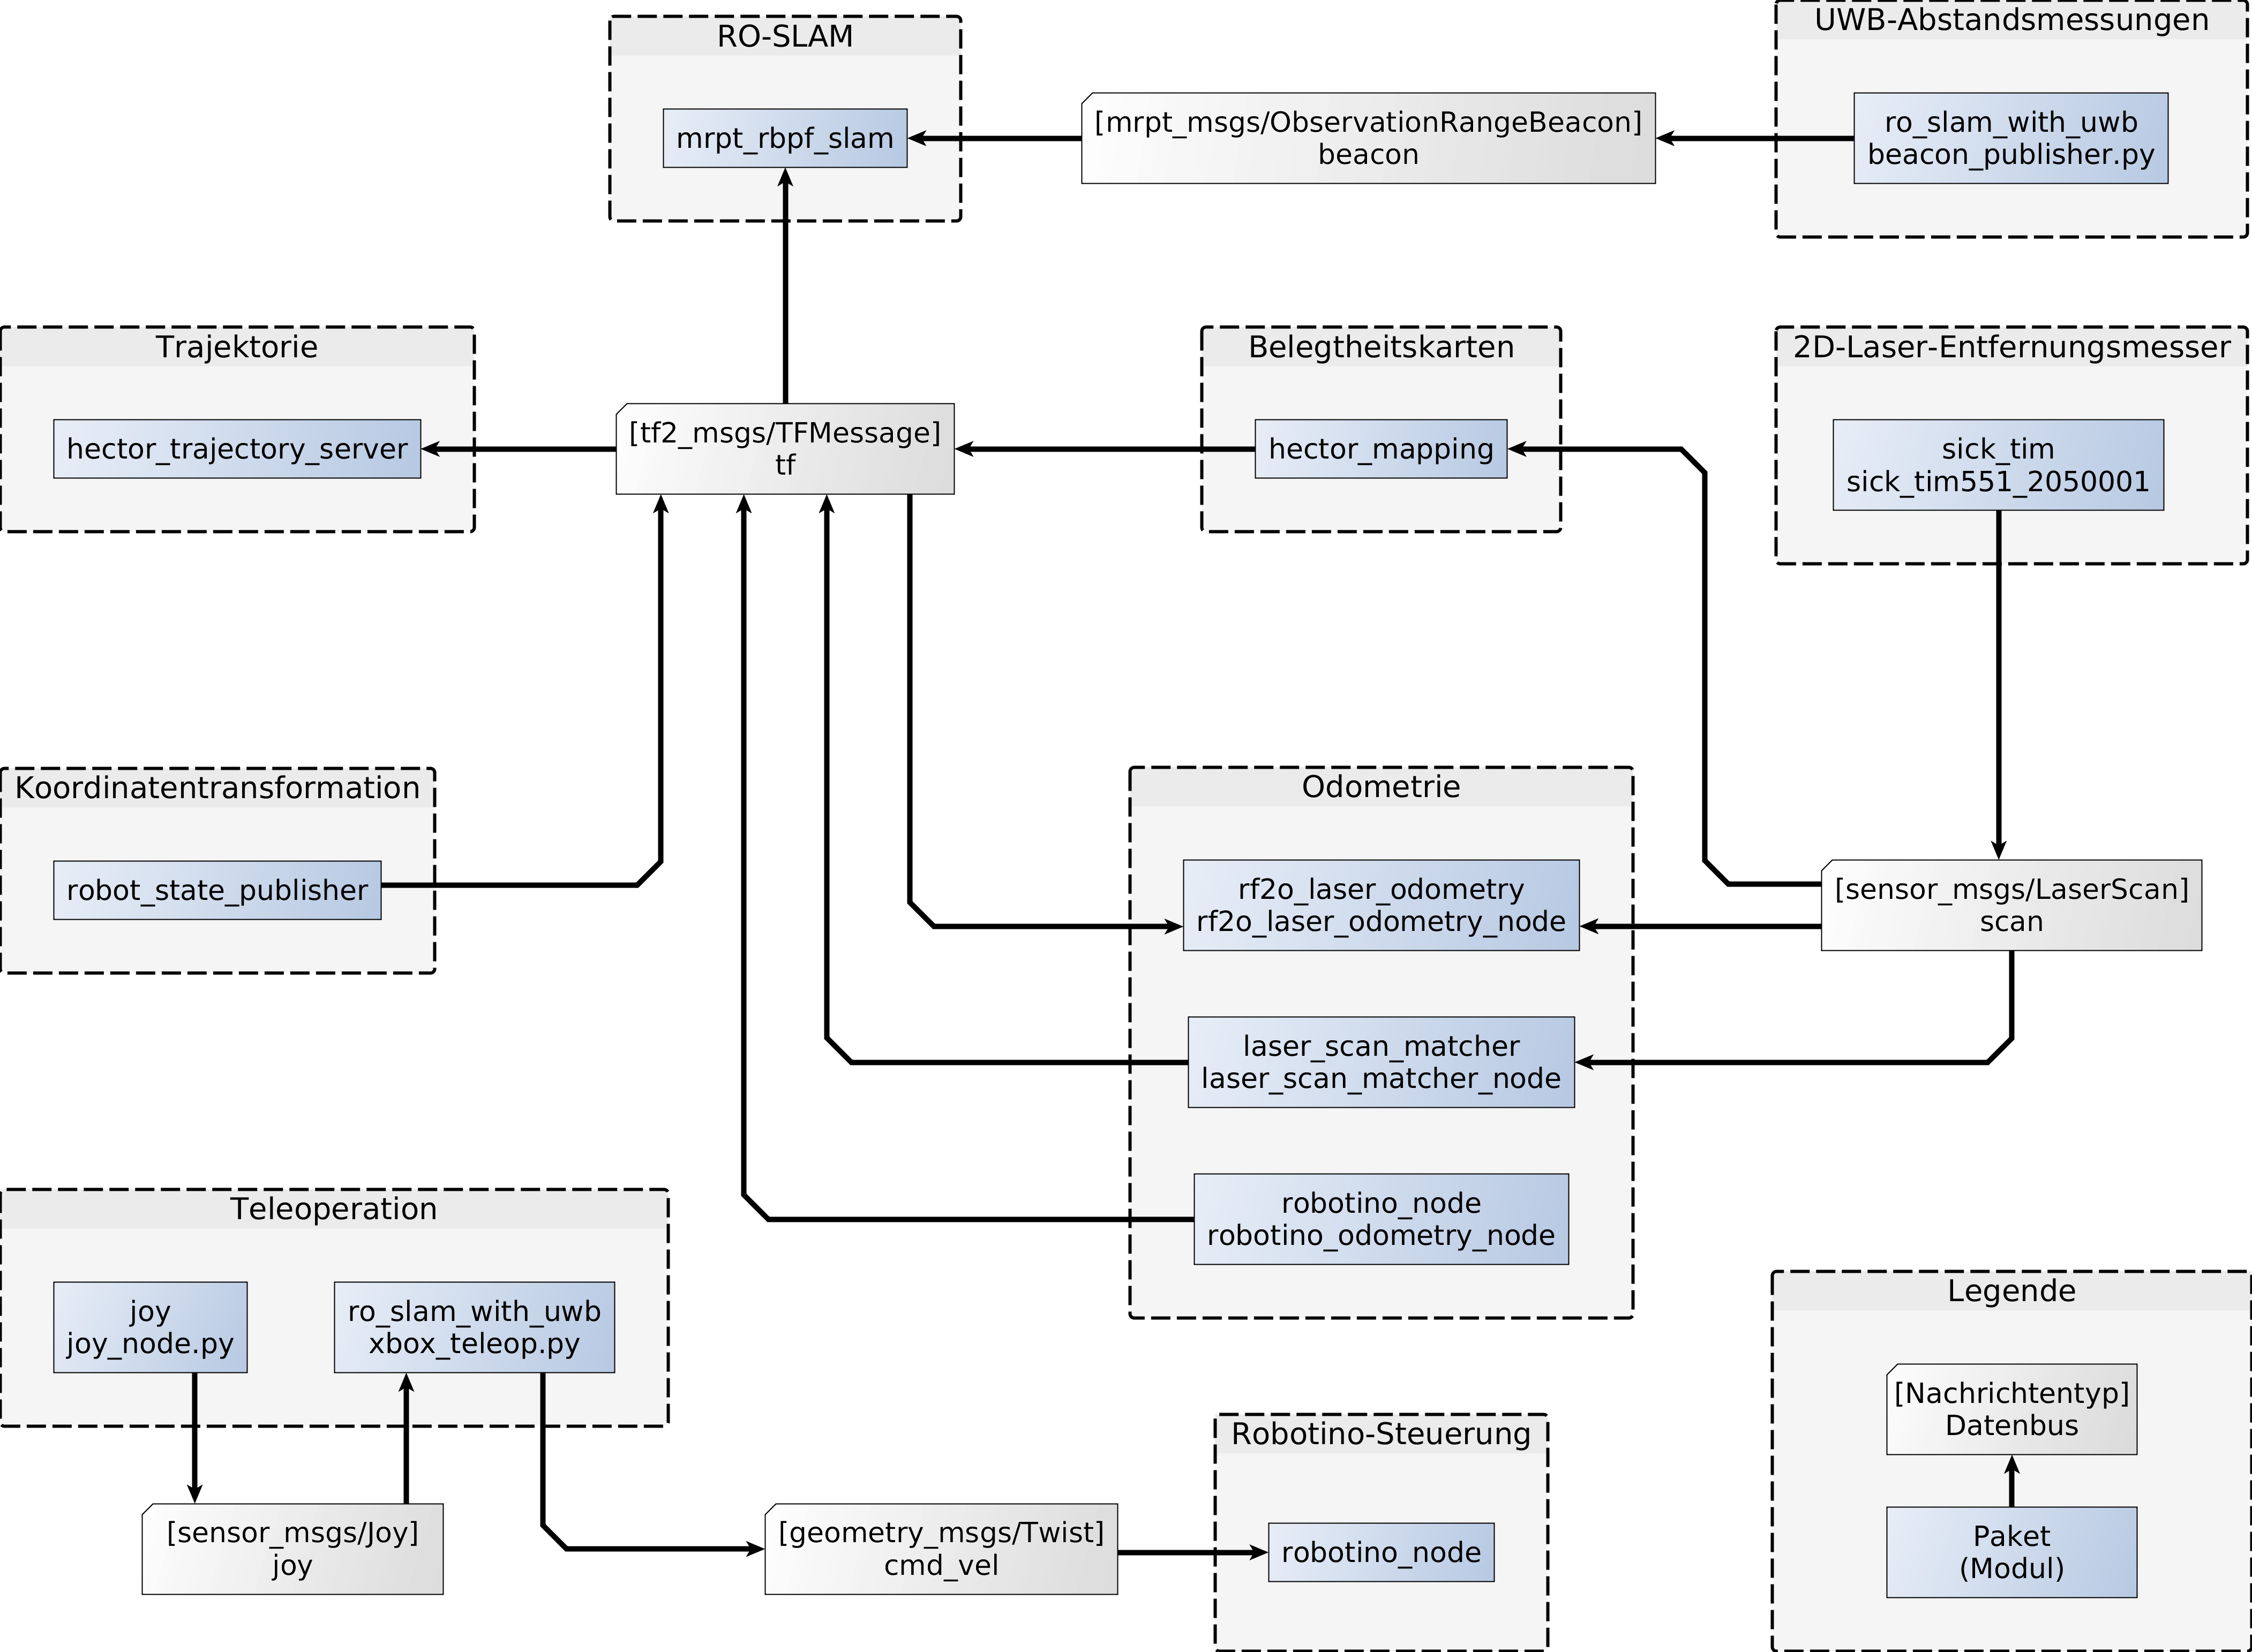
\includegraphics[width=\linewidth]{architektur_grouped}
	\caption{Softwarearchitektur der \glspl{rosm} für den \glsentryshort{roslam}.}
	\label{fig:architektur_grouped}
\end{figure}


%%%%%%%%%%%%%%%%%%%%%%%%%%%%%%%%%%%%%%%%%%%%%%%%%%%%%%%%%%%%%%%%%%%%%%%%%%%%%%%%
%
%
%
%%%%%%%%%%
\subsection{ROS Hauptmodule}


%%%%%%%%%%%%%%%%%%%%%%%%%%%%%%%%%%%%%%%%%%%%%%%%%%%%%%%%%%%%%%%%%%%%%%%%%%%%%%%%
%
%	- \url{http://wiki.ros.org/robotino_node}
%	- Service reset_odometry
%
%%%%%%%%%%
\subsubsection{Robotino-Steuerung}

Zur Steuerung der Roboterplattform muss die Verarbeitungseinheit Befehle zur Steuereinheit des Robotinos schicken. Diese Aufgabe erfüllt das \Gls{rosm} robotino\_node aus dem Paket robotino\_node. Über den Datenbus cmd\_vel können die Geschwindigkeiten in X-/Y-Richtung und um die Z-Achse festgelegt werden. Um den Robotino zu stoppen, müssen alle drei Parameter auf den Wert null gesetzt werden.

Um an die Informationen der Inkrementalgeber zu kommen, muss das \Gls{rosm} robotino\_odometry\_node aus dem Paket robotino\_node gestartet werden. Nach dem Start steht der Datenbus odom mit den aktuellen Werte der Inkrementalgeber zur Verfügung. Zusätzlich sorgt dieses Modul auch für die dynamische Transformation zwischen dem odom und base\_link Koordinatensystem.


%%%%%%%%%%%%%%%%%%%%%%%%%%%%%%%%%%%%%%%%%%%%%%%%%%%%%%%%%%%%%%%%%%%%%%%%%%%%%%%%
%
%	- \url{http://wiki.ros.org/robot_state_publisher}
%	- \url{http://wiki.ros.org/urdf}
%
%%%%%%%%%%
\subsubsection{Koordinatentransformation}

Neben den dynamischen Transformationen besteht die Roboterplattform auch aus vielen statischen Transformationen. Hierzu gehört z.B. die Transformation vom Mittelpunkt der Roboterplattform zum 2D-Laser-Entfernungsmesser oder \Gls{uwbm}. Diese statischen Transformationen werden in einer \Gls{urdf} Datei einmalig gespeichert und dann über das \Gls{rosm} state\_publisher aus dem Paket robot\_state\_publisher zur Laufzeit bereitgestellt, siehe \autoref{fig:rviz_robotino_tf2}.

\begin{figure}
	\centering
	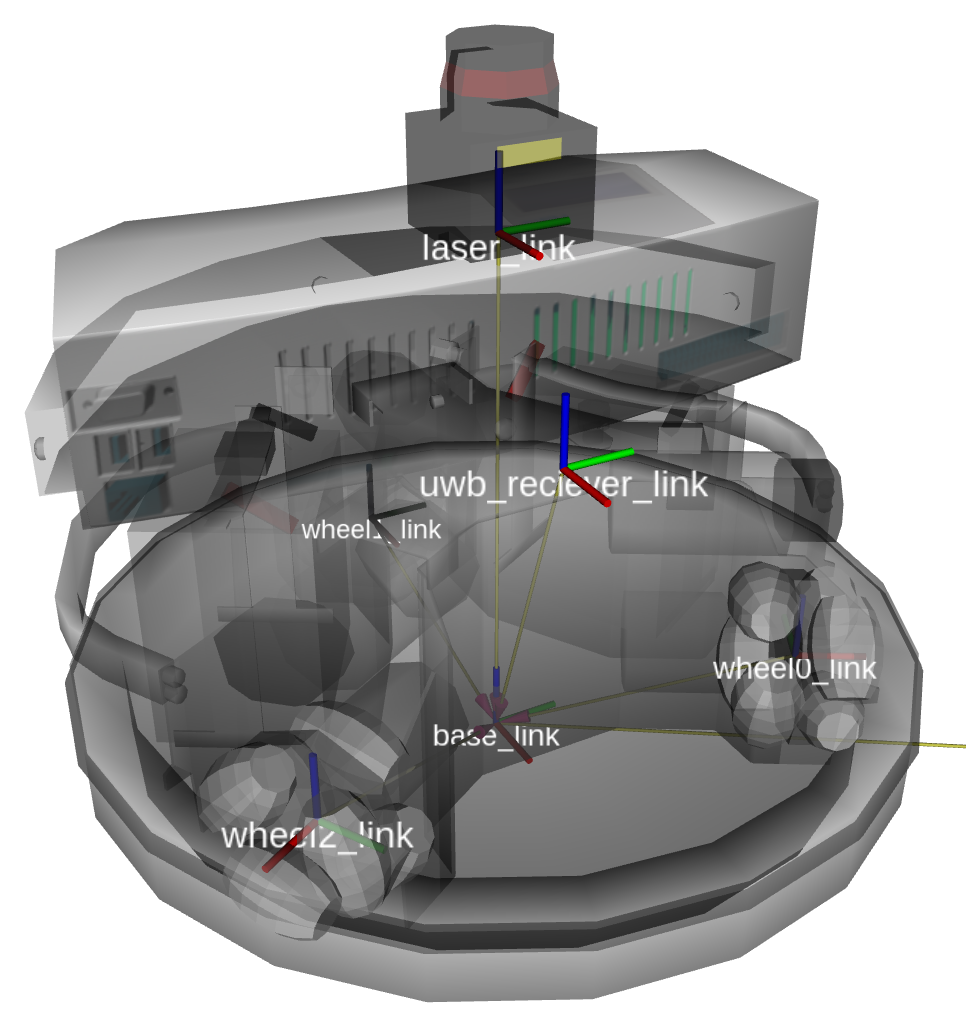
\includegraphics[width=0.5\linewidth]{rviz_robotino_tf2}
	\caption{Statische Transformationen der Roboterplattform.}
	\label{fig:rviz_robotino_tf2}
\end{figure}


%%%%%%%%%%%%%%%%%%%%%%%%%%%%%%%%%%%%%%%%%%%%%%%%%%%%%%%%%%%%%%%%%%%%%%%%%%%%%%%%
%
%	- \url{http://wiki.ros.org/joy}
%
%%%%%%%%%%
\subsubsection{Teleoperation}

Zur Steuerung der Roboterplattform wird ein Xbox Wireless Controller als Eingabegerät verwendet. Zustandsänderungen werden über das \Gls{rosm} joy\_node aus dem Paket joy registriert und über den Datenbus joy bereitgestellt. Das überwachte Eingabegerät wird über den Parameter dev festgelegt.
%, siehe \autoref{lst:joy_node}.

Mit den generischen Daten des Eingabegerätes kann die Roboterplattform nichts anfangen, diese benötigt eine Nachricht vom Typ geometry\_msgs/Twist. Die Transformation zwischen der Nachricht sensor\_msgs/Joy und geometry\_msgs/Twist erfolgt durch das \Gls{rosm} xbox\_teleop.py aus dem Paket ro\_slam\_with\_uwb.


%%%%%%%%%%%%%%%%%%%%%%%%%%%%%%%%%%%%%%%%%%%%%%%%%%%%%%%%%%%%%%%%%%%%%%%%%%%%%%%%
%
%
%
%%%%%%%%%%
\subsubsection{UWB Entfernungsmessung}

Die Entfernungsmessung zwischen dem \Gls{tag} und den vorhandenen \Glspl{anchor} werden durch das \Gls{uwbm} über die \Gls{usb} Schnittstelle bereitgestellt. Die Daten werden dann von dem \Gls{rosm} beacon\_publisher.py aus dem Paket ro\_slam\_with\_uwb aufgefangen und auf den Datenbussen beacon und beacon\_raw veröffentlicht. Der erste Datenbus ist vom Typ mrpt\_msgs/ObservationRangeBeacon und wird von dem \Gls{mrpt} Modul für den \Gls{roslam} benötigt. Der zweite Datenbus wird für die Auswertung der Entfernungsmessung im \autoref{ch:eval} benötigt und ist vom Typ ro\_slam\_with\_uwb/Beacon.


%%%%%%%%%%%%%%%%%%%%%%%%%%%%%%%%%%%%%%%%%%%%%%%%%%%%%%%%%%%%%%%%%%%%%%%%%%%%%%%%
%
%
%
%%%%%%%%%%
\subsection{ROS Hilfsmodule}


%%%%%%%%%%%%%%%%%%%%%%%%%%%%%%%%%%%%%%%%%%%%%%%%%%%%%%%%%%%%%%%%%%%%%%%%%%%%%%%%
%
%	- \url{http://wiki.ros.org/sick_tim}
%
%%%%%%%%%%
\subsubsection{2D-Laser-Entfernungsmesser}

Der 2D-Laser-Entfernungsmesser gehört zu einem der am häufigsten verwendeten Sensoren für die präzise visuelle Erfassen der Umwelt. Für mehrere der nachfolgenden \Gls{rosm} ist eine 2D-Laser-Entfernungsmessung eine zwingende Voraussetzung. Um die Daten dem \Gls{ros} System bereitzustellen wird das \Gls{rosm} sick\_tim551\_2050001 aus dem Paket sick\_tim verwendet. Dieses Modul stellt über den Datenbus scan, mit einer Rate von \SI{15}{\hertz}, Nachrichten vom Typ sensor\_msgs/LaserScan bereit.


%%%%%%%%%%%%%%%%%%%%%%%%%%%%%%%%%%%%%%%%%%%%%%%%%%%%%%%%%%%%%%%%%%%%%%%%%%%%%%%%
%
%	- \url{http://wiki.ros.org/hector_mapping}
%
%%%%%%%%%%
\subsubsection{Belegtheitskarten}

Das erste \Gls{rosm}, das von der 2D-Laser-Entfernungsmessung Gebrauch macht, ist das hector\_mapping aus dem gleichnamigen Paket. Mit diesem Modul können präzise Belegtheitskarten (engl. Occupancy Grid Map) erstellt werden, die für jede Koordinate der Karte festlegen ob diese durch ein Hindernis belegt (schwarz) oder frei (weiß) ist. Bereiche die von Hindernissen verdeckt sind oder außerhalb der Sensorreichweite liegen, werden als unbestimmt (grau) markiert, siehe \autoref{fig:rviz_occupancy_grid_map}. In \Gls{ros} werden Belegtheitskarten mit dem Nachrichtentyp nav\_msgs/OccupancyGrid repräsentiert.

Über die minimale und maximale Sensorreichweite (laser\_min\_dist bzw. laser\_max\_dist) wird festgelegt, welche Messungen für die Kartenerstellung berücksichtigt werden. Es ist sinnvoll die Herstellerangaben von \SI{0.05}{\meter} und \SI{25.0}{\meter} zu verwenden.

Die Auflösung einer Zelle in der Karte wird über den Parameter (map\_resolution) festgelegt. Es eine Auflösung von \SI{0.02}{\meter} pro Zelle verwendet.

\begin{figure}
	\centering
	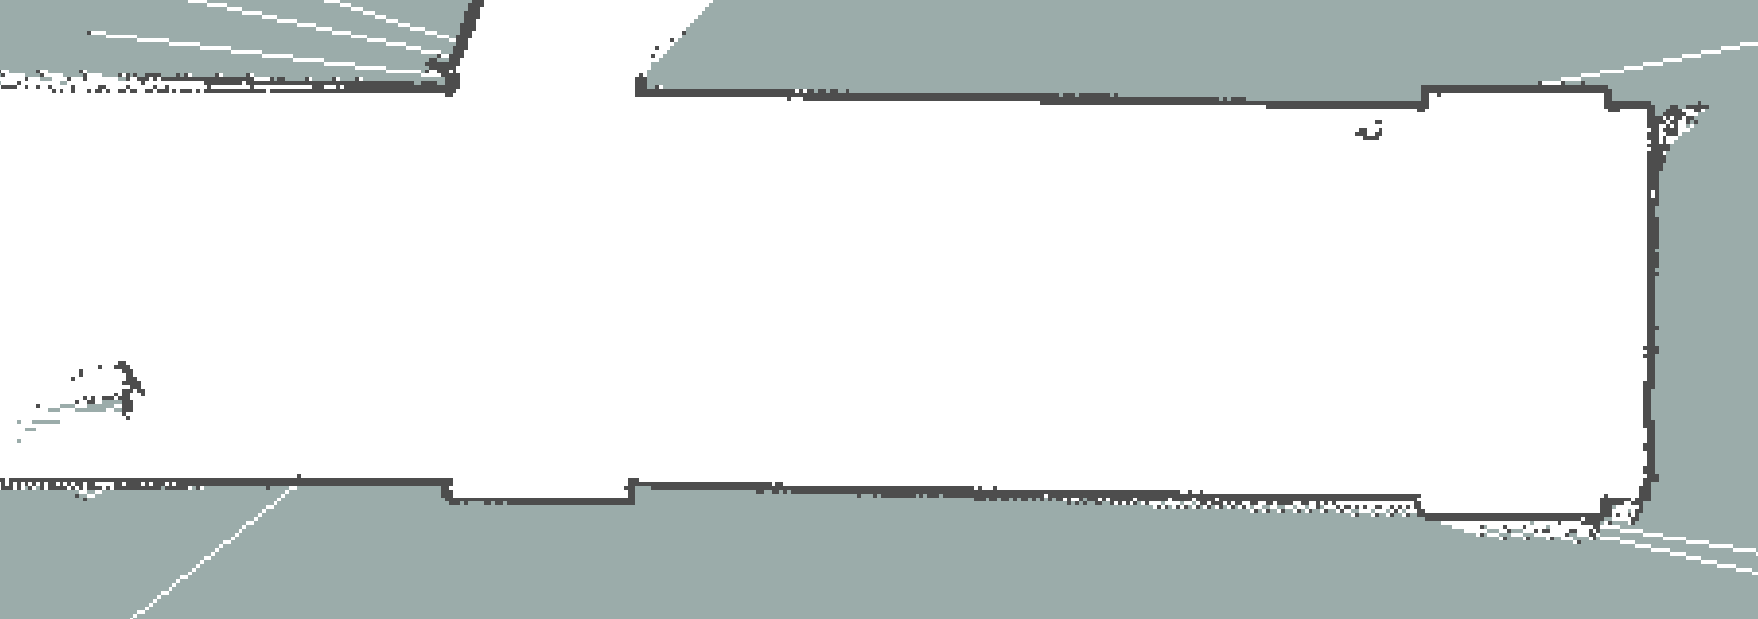
\includegraphics[width=0.9\linewidth]{rviz_occupancy_grid_map}
	\caption{Belegtheitskarte der Messstrecke.}
	\label{fig:rviz_occupancy_grid_map}
\end{figure}
 

%%%%%%%%%%%%%%%%%%%%%%%%%%%%%%%%%%%%%%%%%%%%%%%%%%%%%%%%%%%%%%%%%%%%%%%%%%%%%%%%
%
%	- \url{http://wiki.ros.org/hector_trajectory_server}
%	- \url{http://docs.ros.org/api/nav_msgs/html/msg/Path.html}
%
%%%%%%%%%%
\subsubsection{Trajektorie}

Neben den Entfernungsinformationen wertet der \Gls{roslam} auch die Daten der Odometrie aus. Als Quelle für die Odometrie dienen dabei die Inkrementalgeber der Roboterplattform. Im nächsten Abschnitt werden weitere Quellen für die Odometrie vorgestellt. Um die Güte der Odometrie-Quellen zu vergleichen, wird die verfahrene Trajektorie jeder Quelle benötigt. Diese Informationen werden von dem \Gls{rosm} hector\_trajectory\_server aus dem gleichnamigen Paket bereitgestellt. Die Daten liegen dabei als Nachricht vom Typ nav\_msgs/Path bereit und können in die Belegtheitskarte integriert werden, siehe \autoref{fig:rviz_trajektorie}.

\begin{figure}
	\centering
	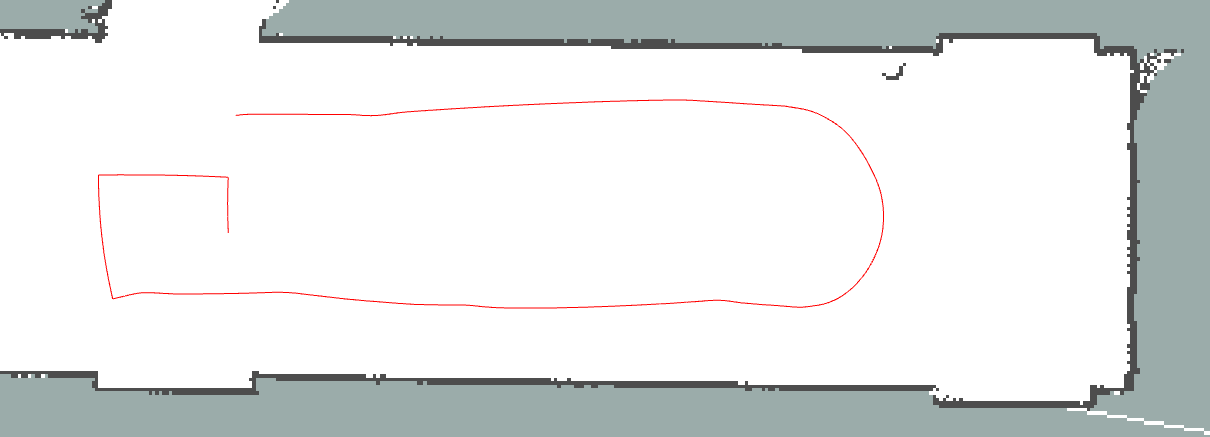
\includegraphics[width=0.9\linewidth]{rviz_trajektorie}
	\caption{Trajektorie einer Messfahrt der Roboterplattform.}
	\label{fig:rviz_trajektorie}
\end{figure}


%%%%%%%%%%%%%%%%%%%%%%%%%%%%%%%%%%%%%%%%%%%%%%%%%%%%%%%%%%%%%%%%%%%%%%%%%%%%%%%%
%
%	- \url{http://wiki.ros.org/rf2o}
%	- \url{http://wiki.ros.org/laser_scan_matcher}
%
%%%%%%%%%%
\subsubsection{Laser-Odometrie}

Wie bereits im vorherigen Abschnitt erwähnt, werden hier zwei weitere Quellen für die Odometrie vorgestellt. Beide \Glspl{rosm} nutzen nur die Daten der 2D-Laser-Entfernungsmessung, um eine Schätzung für die aktuelle Pose zu erstellen.

Bei dem ersten \gls{rosm} handelt es sich um den laser\_scan\_matcher\_node aus dem Paket laser\_scan\_matcher. Hierbei handelt es sich um eine Variante des \gls{icp} Verfahrens, welches versucht eine Transformation zwischen den Punkt einer Oberfläche aus den vorherigen und aktuellen Sensordaten zu finden. Jedoch wird anstatt einer Punkt-zu-Punkt- eine Punkt-zu-Linie-Metrik für die Minimierung verwendet. \cite{censi2008icp} Dieses Verfahren wird im Folgenden nur noch als LSM Verfahren bezeichnet.

Bei dem zweiten \gls{rosm} handelt es sich um den rf2o\_laser\_odometry\_node aus dem Paket rf2o\_laser\_odometry. Hierbei handelt es sich um eine Implementierung des \gls{rf2o} Verfahrens, bei dem jeder beobachtete Punkt des Sensors als eine Funktion der Geschwindigkeit des Sensors modelliert wird. Die Bewegung des Sensors wird dann aus der Minimierung der Dichteformulierung aller Punkt-Funktionen berechnet. \cite{jaimez2016planar}


%%%%%%%%%%%%%%%%%%%%%%%%%%%%%%%%%%%%%%%%%%%%%%%%%%%%%%%%%%%%%%%%%%%%%%%%%%%%%%%%
%
%	- \url{https://www.mrpt.org}
%	- \url{http://wiki.ros.org/mrpt_slam}
%	- \url{http://wiki.ros.org/mrpt_navigation}
%	- \url{https://www.mrpt.org/tutorials/slam-algorithms/rangeonly_slam/}
%		- Bayesian range-only SLAM (RO-SLAM) with SOGs
%	- \url{http://mrpt.ual.es/reference/devel/classmrpt_1_1slam_1_1_c_metric_map_builder_r_b_p_f.html}
%		- mrpt::slam::CMetricMapBuilderRBPF Class Reference
%		- It is actually a front-end to the class mrpt::slam::CMetricMapBuilderRBPF.
%		- All the parameters to the algorithm are passed through a configuration file in the command line.
%		- The filter processes actions and observations from a rawlog file and optionally generates a number of files describing the evolution of the filter and the maps.
%
%%%%%%%%%%
\subsection{MRPT}

Bei dem \Gls{mrpt} Framework handelt es sich um eine Bibliothek die Datenstrukturen und Algorithmen aus dem aktiven Forschungsbereich der Robotik bereitstellt. Dadurch ist eine schnelle Umsetzung neuer Algorithmen, sowie der Vergleich mit bereits bestehenden möglich. Zu den verfügbaren Datenstrukturen zählen die Basisdatentypen der linearen Algebra bis hin zu den komplexeren Datentypen der Robotik wie z.B. die Belegtheitskarten. Zur direkten Verwendung existieren viele Algorithmen aus den Bereichen der \Gls{slam}-Algorithmen, des Maschinellen Sehen (engl. Computer Vision) und der Pfad- und Bewegungsplanung (engl. Path/Motion Planning).

Aus dem Bereich der \Gls{roslam} Algorithmen sind die Verfahren aus den Veröffentlichungen \citetitle{blanco2008pure} und \citetitle{blanco2008efficient} implementiert, siehe \autoref{sec:blanco2008pure} und \ref{sec:blanco2008efficient}.

Um die \Gls{roslam} Algorithmen aus dem \Gls{mrpt} Framework zu nutzen, wird das \Gls{rosm} mrpt\_rbpf\_slam aus dem Paket mrpt\_rbpf\_slam benötigt. Mit dem Parameter \mbox{ini\_filename} wird der Dateipfad zu der Konfigurationdatei für die \Gls{roslam} Algorithmen angegeben und über den sensor\_source Parameter werden die Datenquellen für den \Gls{roslam} definiert. Hierbei ist es möglich sowohl die Entfernungsmessungen der \Gls{uwbm} als auch die der 2D-Laser-Entfernungsmesser anzugeben. Von der letzten Datenquelle wird kein gebrauch gemacht, da diese Transformationen veröffentlicht, die mit den bereits bestehenden Koordinatensystemen kollidiert. Über die Datenbusse particlecloud und \mbox{particlecloud\_beacons} werden die Positionsschätzungen für die Roboterplattform und die \Glspl{uwbm} veröffentlicht, siehe \autoref{fig:rviz_robot_and_beacon_estimate}.

\begin{figure}
	\centering
	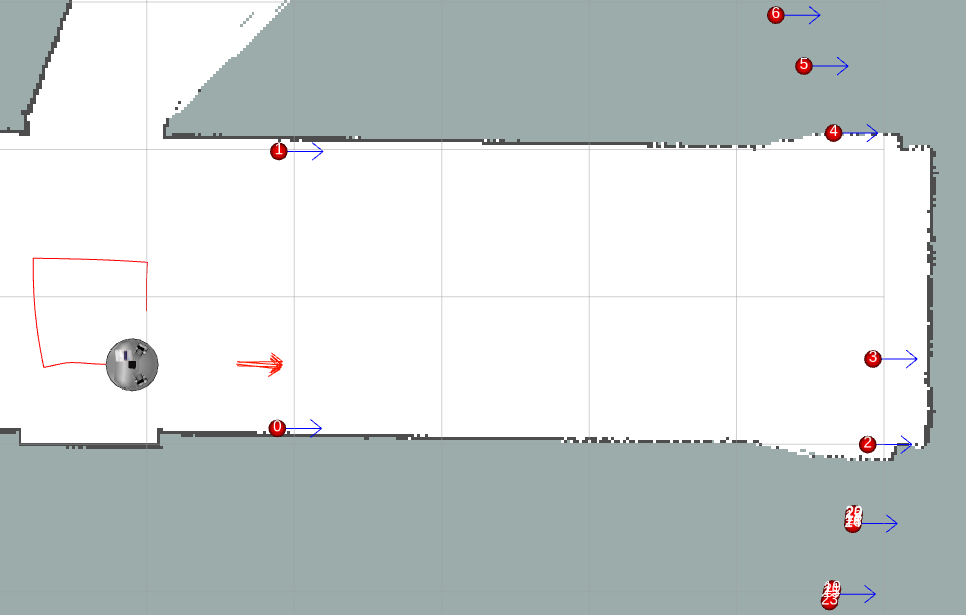
\includegraphics[width=0.9\linewidth]{rviz_robot_and_beacon_estimate}
	\caption{Positionsschätzung für die Roboterplattform mit roten Pfeilen und für die \Glspl{uwbm} mit blauen Pfeilen.}
	\label{fig:rviz_robot_and_beacon_estimate}
\end{figure}

Nach der Konfiguration der \Gls{ros} Seite müssen noch Einstellungen für den \Gls{roslam} festgelegt werden. Hier muss die Konfigurationsdatei, die in dem \Gls{ros} Parameter ini\_filename hinterlegt ist, bearbeitet werden. Das \Gls{mrpt} Framework verfügt über einen eigenen Abspielmechanismus für aufgezeichnete Messungen. Dieser wird nicht verwendet, da \Gls{ros} über einen eigenen Mechanismus verfügt. Folglich wird der Parameter rawlog\_file auf einen leeren Wert gesetzt werden. Auch verfügt \Gls{ros} über eine eigene Visualisierungslösung, daher wird die grafische Anzeige des \Gls{mrpt} Frameworks über den Parameter SHOW\_PROGRESS\_IN\_WINDOW=0 deaktiviert. Um zwischen den beiden \Gls{roslam} Verfahren zu wechseln, wird der Parameter insertAsMonteCarlo angepasst werden.


	%%%%%%%%%%%%%%%%%%%%%%%%%%%%%%%%%%%%%%%%%%%%%%%%%%%%%%%%%%%%%%%%%%%%%%%%%%%%%%%%
%
%
%
%%%%%%%%%%
\chapter{Evaluation}\label{ch:eval}


%%%%%%%%%%%%%%%%%%%%%%%%%%%%%%%%%%%%%%%%%%%%%%%%%%%%%%%%%%%%%%%%%%%%%%%%%%%%%%%%
%
%	- Start 13:50-23:50, 12:50-20:00 => 10+7 => 17 Stunden
%
%%%%%%%%%%
\section{Batterielaufzeit}

Beim Test der Batterielaufzeit wurden zwei \gls{uwbm} in einem Abstand von \SI{4.7}{\metre} aufgestellt. Beide \gls{uwbm} hatten eine direkte \gls{los} zu einandern. Über den kompletten Zeitraum wurden Entfernungsmessungen mit einer Rate von \SI{10}{\hertz} durchgeführt. Als Testprogramme wurden dabei DW1000Ranging\_ANCHOR und DW1000Ranging\_TAG aus dem GitHub Projekt \cite{Trojer2015} verwendet.

Der \Gls{anchor} hatte nach ca. \SI{17}{\hour} seinen Dienst eingestellt, wenig später folgte Ihm der \Gls{tag}. Deutlich höhere Batterielaufzeiten können dadurch erzielt werden, dass die Senderate reduziert wird und die Stromsparfunktionen sowohl des DWM1000 als auch des ATmega328/P genutzt werden.


%%%%%%%%%%%%%%%%%%%%%%%%%%%%%%%%%%%%%%%%%%%%%%%%%%%%%%%%%%%%%%%%%%%%%%%%%%%%%%%%
%
%	- 3-sigma
%		- https://www.easycalculation.com/statistics/learn-three-sigma.php
%		- https://bizfluent.com/how-5214886-calculate-sigma.html
%		- https://stackoverflow.com/questions/28699342/calculate-the-3rd-standard-deviation-for-an-array
%
%%%%%%%%%%
\section{Kalibierung}

Um die Antennenverzögerung pro \Gls{uwbm} zu bestimmen, werden zwei Kalibriervorgänge durchgeführt. Der erste Kalibriervorgang orientiert sich an den Herstellervorgaben aus \cite{decawave2014calibration}. Dazu werden drei \Glspl{uwbm} an die Spitzen eines gleichseitigen Dreieckes positioniert. Um das Dreieck zu konstruieren, wird in der Mitte des Dreiecks eine ausgemessene Maurerschnur befestigt, darüber wird eine Winkelschablone gelegt und dann reihum die Spitzen es Dreiecks auf dem Boden eingezeichnet, siehe \autoref{fig:calibration_triangle2}. Die Seitenlänge $a \approx \SI{1.73}{\meter}$ wird dabei aus dem Umkreisradius $r_u = \SI{1}{\meter}$ mit der \autoref{eq:dreieck_seitenlaenge_aus_umkreis} berechnet.

\begin{figure}
	\centering
	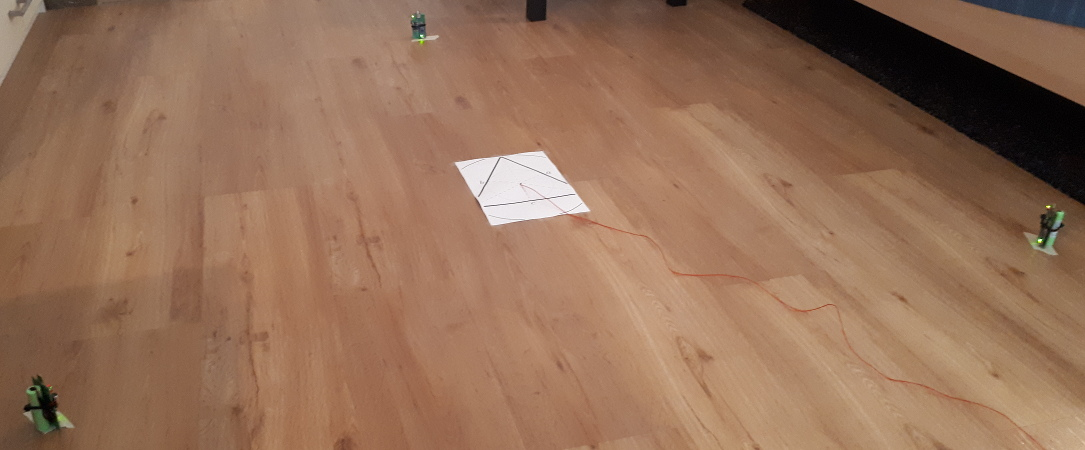
\includegraphics[width=0.9\linewidth]{calibration_triangle2}
	\caption{Versuchsaufbau für die Kalibierung von drei \Glsuseri{uwbm}.}
	\label{fig:calibration_triangle2}
\end{figure}

Initial wird die Antennenverzögerung bei allen \Glsuseri{uwbm} auf null gesetzt und danach reihum von jedem \Gls{uwbm} eintausend Entfernungsmessungen zu den beiden benachbarten \Glsuseri{uwbm} durchgeführt. Insgesamt entstehen dabei sechstausend Datensätze, die mittels dem LGS- bzw. des DecaWave Kalibrierungsverfahren ausgewertet werden, siehe \autoref{tab:calibration_antenna_delay_results}

Das LGS Kalibrierungsverfahren lieferte für jeden Durchlauf reproduzierbare Ergebnisse. Da jedes \Gls{uwbm} herstellungsbedingte Unterschiede aufweist, ist es Plausibel das alle Antennenverzögerungen in einem ähnlichen Wertebereich liegen. Anders sieht es bei dem DecaWave Kalibrierungsverfahren aus. Hier ergeben sich für jeden Durchlauf andere Wertekombinationen, bedingt durch die Zufallskomponente bei der Erstellung der Kandidatenliste. Diese Verhalten von Genetischen Algorithmen ist bekannt und muss daher bei der Auswahl der Wertekombinationen berücksichtigt werden. Am Beispiel der Spalte DecaWave 1 wird es sehr deutlich. Hier beträgt der Unterschied zwischen dem größten und kleinsten Wert ca. \SI{23}{\ns} und entspricht damit einer Abweichung von ca. \SI{6}{\meter} zwischen diesen beiden \Glsuseri{uwbm}.

\begin{table}
	\centering
	\begin{tabular}{||c||c||ccc||}
\hline
\Gls{uwbm} & LGS & DecaWave & DecaWave 1 & DecaWave 2 \\
& [\si{\nano\second}] & [\si{\nano\second}] & [\si{\nano\second}] & [\si{\nano\second}] \\
\hline
\hline
176 & \num{257.45} & \num{242.48} & \num{232.21} & \num{254.50} \\
177 & \num{257.49} & \num{238.47} & \num{249.38} & \num{254.73} \\
178 & \num{257.11} & \num{257.17} & \num{255.36} & \num{215.07} \\
\hline
% Alte Darstellung
%176 & 16451 & 15494 & 14838 & 15912 & 16262 \\
%177 & 16453 & 15238 & 15935 & 15805 & 16277 \\
%178 & 16429 & 16433 & 16317 & 15131 & 13743 \\
	\end{tabular}
	\caption{Berechnete Werte für die Antennenverzögerung pro \glsentrytext{uwbm}.}
	\label{tab:calibration_antenna_delay_results}
\end{table}

Die Wertekombinationen aus den Spalten LGS und DecaWave werden abwechselnd als Antennenverzögerungen in die \Glspl{uwbm} eingetragen und für jede Spalte jeweils eine weitere Messreihe, wie oben beschrieben, aufgezeichnet. Die Ergebnisse sind in der \autoref{tab:calibration_range_results}\footnotemark{} aufgeführt.

\begin{table}
	\centering
	\begin{tabular}{||c||cc||ccc|cc||}
\hline
Kalibrierung & Tag & Anker & Entfernung & $\overline{x}$ & $\sigma$ & Min & Max \\
 & & & [\si{\meter}] & [\si{\meter}] & [\si{\meter}] & [\si{\meter}] & [\si{\meter}] \\
\hline
\hline
Keine & 176 & 177 & \num{1.732} & \num{156.108} & \num{0.018} & \num{156.050} & \num{156.170} \\
Keine & 176 & 178 & \num{1.732} & \num{155.929} & \num{0.021} & \num{155.870} & \num{156.000} \\
Keine & 177 & 176 & \num{1.732} & \num{156.106} & \num{1.025} & \num{156.020} & \num{188.470} \\
Keine & 177 & 178 & \num{1.732} & \num{156.016} & \num{0.023} & \num{155.930} & \num{156.090} \\
Keine & 178 & 176 & \num{1.732} & \num{156.067} & \num{0.022} & \num{156.010} & \num{156.130} \\
Keine & 178 & 177 & \num{1.732} & \num{155.997} & \num{0.019} & \num{155.930} & \num{156.060} \\
\hline
LGS & 176 & 177 & \num{1.732} & \num{1.695} & \num{0.019} & \num{1.640} & \num{1.750} \\
LGS & 176 & 178 & \num{1.732} & \num{1.795} & \num{0.022} & \num{1.740} & \num{1.880} \\
LGS & 177 & 176 & \num{1.732} & \num{1.656} & \num{0.017} & \num{1.590} & \num{1.700} \\
LGS & 177 & 178 & \num{1.732} & \num{1.751} & \num{0.023} & \num{1.670} & \num{1.810} \\
LGS & 178 & 176 & \num{1.732} & \num{1.773} & \num{0.026} & \num{1.700} & \num{1.850} \\
LGS & 178 & 177 & \num{1.732} & \num{1.712} & \num{0.020} & \num{1.660} & \num{1.780} \\
\hline
DecaWave & 176 & 177 & \num{1.732} & \num{11.883} & \num{0.020} & \num{11.820} & \num{11.950} \\
DecaWave & 176 & 178 & \num{1.732} & \num{6.261} & \num{0.021} & \num{6.200} & \num{6.340} \\
DecaWave & 177 & 176 & \num{1.732} & \num{11.857} & \num{0.015} & \num{11.810} & \num{11.900} \\
DecaWave & 177 & 178 & \num{1.732} & \num{7.406} & \num{0.023} & \num{7.340} & \num{7.480} \\
DecaWave & 178 & 176 & \num{1.732} & \num{6.182} & \num{0.025} & \num{6.100} & \num{6.270} \\
DecaWave & 178 & 177 & \num{1.732} & \num{7.458} & \num{0.019} & \num{7.390} & \num{7.520} \\
\hline
	\end{tabular}
	\caption[Stochastische Eigenschaften der \Glspl{uwbm} ohne und mit Antennenkalibrierung bei einem Abstand von \SI{1.73}{\meter}.]{Stochastische Eigenschaften der \Glspl{uwbm} ohne und mit Antennenkalibrierung bei einem Abstand von \SI{1.73}{\meter}.}
	\label{tab:calibration_range_results}
\end{table}

\footnotetext{Bei der Standardabweichung von über einem Meter handelt es sich um einen einzelnen Messfehler in der Messreihe.}

Mit einer initalen Antennenverzögerung von null beträgt die gemessene Entfernung zwischen zwei \Glsuseri{uwbm} ca. \SI{156}{\meter} bei einer tatsächenlichen Entfernung von ca. \SI{1.73}{\meter}. Eine Standardabweichung von ca. \SI{2}{\centi\meter} entspricht dabei den Produkteigenschaften mit denen DecaWave wirbt.

Werden die Antennenverzögerung aus der LGS Kalibrierungsverfahren benutzt, verbleibt die Standardabweichung in der gleichen Größenordnung wie im unkalibrierten Zustand. Jedoch nähert sich jetzt die gemessenen Entfernungen der tatsächlichen sehr stark an und bildet diesen sehr gut ab. Ganz im Gegensatz zu dem DecaWave Kalibrierungsverfahren.


In der \autoref{fig:calibration_histograms} wurden die gemessenen Entfernungen als Histogramm dargestellt. Gut zu erkennen ist die Normalverteilung der Messwerte um den Mittelwert.

\begin{figure}
	\centering
	\begin{subfigure}[b]{0.32\linewidth}
		\centering
		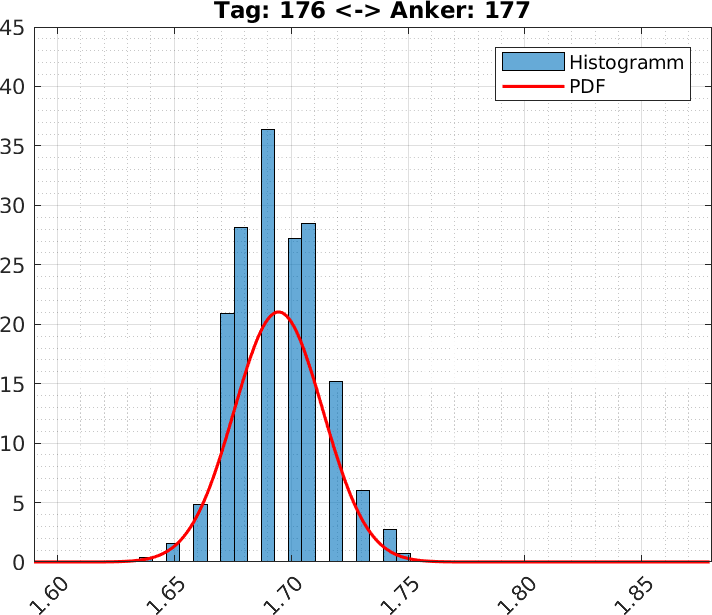
\includegraphics[width=\linewidth]{calibration_histogram_176_177}
	\end{subfigure}
	\hfill
	\begin{subfigure}[b]{0.32\linewidth}
		\centering
		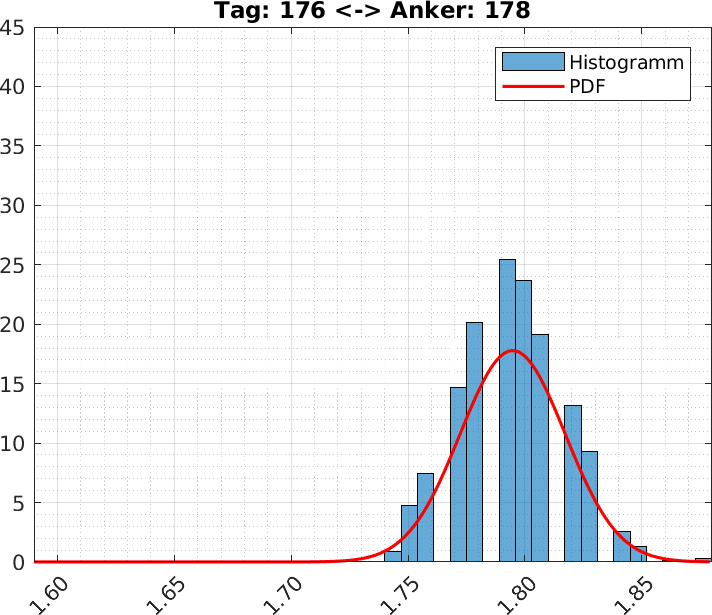
\includegraphics[width=\linewidth]{calibration_histogram_176_178}
	\end{subfigure}
	\hfill
	\begin{subfigure}[b]{0.32\linewidth}
		\centering
		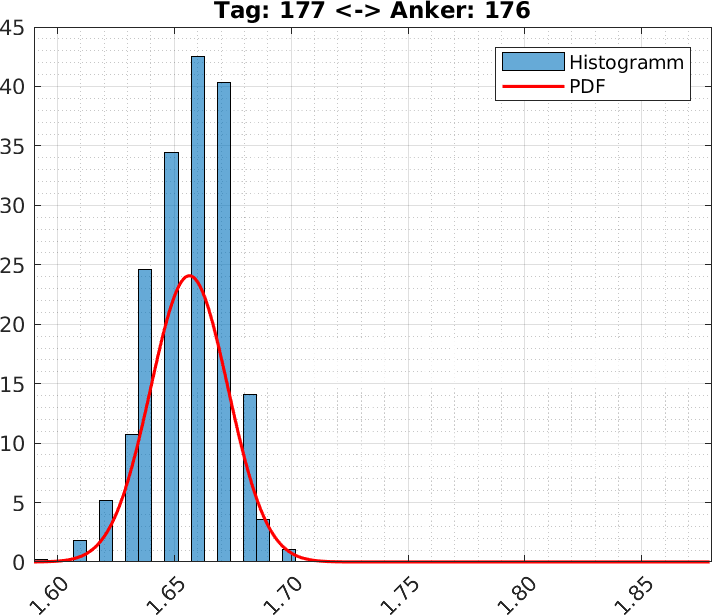
\includegraphics[width=\linewidth]{calibration_histogram_177_176}
	\end{subfigure}
	\par
	\bigskip
	\begin{subfigure}[b]{0.32\linewidth}
		\centering
		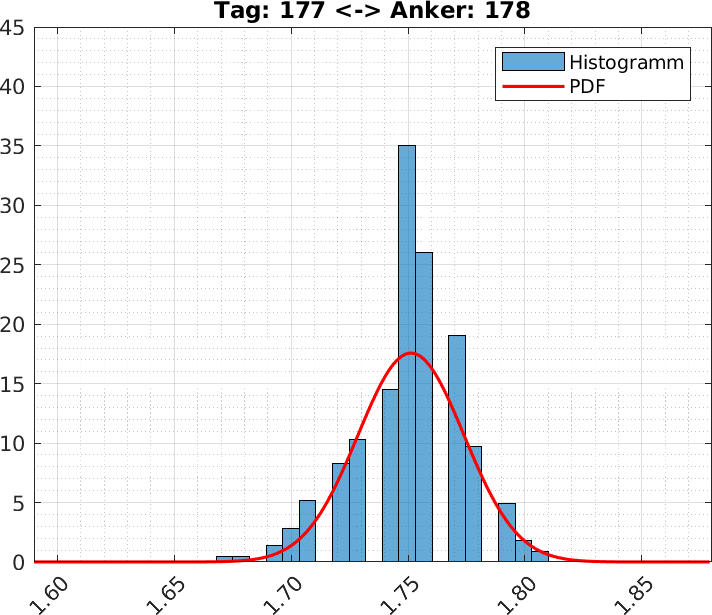
\includegraphics[width=\linewidth]{calibration_histogram_177_178}
	\end{subfigure}
	\hfill
	\begin{subfigure}[b]{0.32\linewidth}
		\centering
		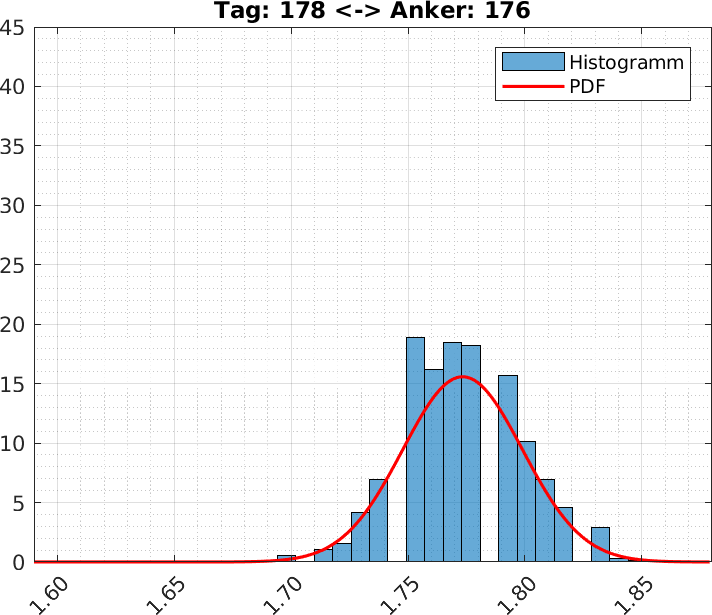
\includegraphics[width=\linewidth]{calibration_histogram_178_176}
	\end{subfigure}
	\hfill
	\begin{subfigure}[b]{0.32\linewidth}
		\centering
		\includegraphics[width=\linewidth]{calibration_histogram_178_177}
	\end{subfigure}
	\caption{Histogramm und Wahrscheinlichkeitsdichtefunktion der kalibrierten Entfernungsmessungen.}
	\label{fig:calibration_histograms}
\end{figure}

Im zweiten Kalibriervorgang werden alle fünf \Glspl{uwbm} eingeschlossen. Jetzt reicht ein Dreieck nicht mehr aus, statt dessen wird ein regelmäßiges Fünfeck verwendet, siehe \autoref{fig:calibration_pentagram2}. Dieses lässt sich mathematisch ähnlich gut beschreiben wie das Dreieck. Aus der Seitenlänge $a = \SI{4.5}{\meter}$, zwischen zwei benachbarten Spitzen, wird über die \autoref{eq:fuenfeck_diagonale} die Entfernung $d$, zwischen den diagonalen Spitzen, berechnet. Der Umkreisradius $r_u$ ergibt sich aus der \autoref{eq:fuenfeck_umkreisradius}.

\begin{figure}
	\centering
	\includegraphics[width=0.9\linewidth]{calibration_pentagram2}
	\caption{Versuchsaufbau für die Kalibierung von fünf \glsuseri{uwbm}.}
	\label{fig:calibration_pentagram2}
\end{figure}

Für das regelmäßige Fünfeck wurde nur noch das LGS Kalibrierungsverfahren verwendet, die Antennenverzögerungen pro \Gls{uwbm} sind dabei in der \autoref{tab:calibration_pentagramm_antenna_delay_results} aufgeführt.

\begin{table}
	\centering
	\begin{tabular}{||c||c||}
\hline
\Gls{uwbm} & LGS \\
 & [\si{\nano\second}] \\
\hline\hline
176 & \num{257.30} \\
177 & \num{256.67} \\
178 & \num{256.67} \\
179 & \num{256.41} \\
180 & \num{257.20} \\

% Alte Darstellung
%176 & 16441 \\
%177 & 16401 \\
%178 & 16401 \\
%179 & 16384 \\
%180 & 16435 \\
\hline
	\end{tabular}
	\caption{Berechnete Werte für die Antennenverzögerung pro \glsentryshort{uwbm} für das regelmäßige Fünfeck.}
	\label{tab:calibration_pentagramm_antenna_delay_results}
\end{table}


%%%%%%%%%%%%%%%%%%%%%%%%%%%%%%%%%%%%%%%%%%%%%%%%%%%%%%%%%%%%%%%%%%%%%%%%%%%%%%%%
%
%	- Wie verändert sich die Genauigkeit der Entfernungsmessung bei einer direkten Sichtverbindung (engl. Line-of-sight (LOS)) und indirekten Sichtverbindung (engl. Non-line-of-sight (NLOS))?
%	- Stochastik
%		- https://matheguru.com/stochastik/mittel-durchschnitt-und-lageparameter.html
%		- https://matheguru.com/stochastik/standardabweichung.html
%		- https://matheguru.com/stochastik/standardfehler.html

%
%%%%%%%%%%
\section{Entfernungsmessung}

Um die Charakteristik der Entfernungsmessung zu bestimmen, wird eine \Gls{los}- und drei \Gls{nlos} Messreihen aufgezeichnet. Jede Messreihe beginnt bei einer Entfernung von einem Meter zwischen \Gls{tag} und \Gls{anchor}. Pro Entfernung werden jeweils fünfhundert Messwerte aufgezeichnet. Danach wird die Entfernung um einen halben Meter erhöht, indem der \Gls{anchor} verschoben wird. Dies erfolgt solange bis eine Entfernung von neun Meter erreicht ist. Somit enthält jede Messreihe siebzehn Entfernungen mit achttausendfünfhundert Entfernungsmessungen.

Bei der ersten \Gls{nlos} Messreihe wird ein \SI{19x12x10}{\centi\meter} großer, mit Wasser gefüllter Kunststoffbehälter in einem Abstand von \SI{2}{\centi\meter} vor der \Gls{uwb} Antenne platziert, siehe \autoref{fig:entfernungsmessung_versuchsaufbau_20180120_133013}. Bei den letzten zwei \Gls{nlos} Messreihen wird ein \SI{44x25}{\centi\meter} großes Aluminiumblech mit einer Dicke von \SI{0.5}{\milli\meter} vor die \Gls{uwb} Antenne platziert, jeweils in einem Abstand von \SI{5}{\centi\meter} und \SI{50}{\centi\meter}, siehe \autoref{fig:entfernungsmessung_versuchsaufbau_20180120_140118} und \autoref{fig:entfernungsmessung_versuchsaufbau_20180120_122434}.


Das auffälligste Merkmal der \Gls{los}- als auch der \Gls{nlos} Entfernungsmessungen ist die systematische Verschiebung aller Messwerte um ca. \SI{20}{\centi\meter} deren Ursache ungeklärt bleibt, siehe \autoref{fig:entfernungsmessung_2018_01_20}.

Bei der \Gls{los} Messreihe beträgt die Standardabweichung, wie bereits bei der Kalibrierung, ca. \SI{2}{\centi\meter}. Mit steigender Entfernung steigt auch die Standardabweichung von ca. \SI{1.8}{\centi\meter} bei einem Meter auf ca. \SI{2.3}{\centi\meter} bei neun Meter an. Größere Ausreißer sind bei den Messwerten nicht vorhanden, siehe \autoref{fig:entfernungsmessung_2018_01_20_los} und \autoref{tab:entfernungsmessung_2018_01_20_los}.

In der \autoref{fig:entfernungsmessung_2018_01_20_nlos_water} ist deutlich zu erkennen, das Wasser einen sehr störenden Einfluss auf die Entfernungsmessung ausübt. Die Messwerte streuen über einen sehr großen Bereich, das spiegelt sich auch in der Standardabweichung, die im besten Fall ca. \SI{5}{\centi\meter} und im schlimmsten Fall ca. \SI{34}{\centi\meter} beträgt, siehe \autoref{tab:entfernungsmessung_2018_01_20_nlos_water}.

Ähnlich verhält es sich bei der \Gls{nlos} Messreihe mit einem Aluminiumblech, das sehr nah vor der \Gls{uwb} Antenne platziert wurde, siehe \autoref{fig:entfernungsmessung_2018_01_20_nlos_metal2} und \autoref{tab:entfernungsmessung_2018_01_20_nlos_metal2}. Einzig im Bereich von zwei bis fünf Meter beträgt die Standardabweichung ca. \SI{2}{\centi\meter}.

Keinen besonders großen Einfluss hat das Aluminiumblech, wenn es sich in einer Entfernung von \SI{50}{\centi\meter} befindet, siehe \autoref{tab:entfernungsmessung_2018_01_20_nlos_metal}. Die Werte der Standardabweichung ähneln der \Gls{los} Messreihe. Nur im Bereich zwischen achteinhalb und neun Meter steigt die Standardabweichung auf einen Wert von ca. \SI{30}{\centi\meter} an. Dies könnte darauf zurückzuführen sein, das im hinteren Bereich des Raums Metallstühle auf den Tischen standen, siehe \autoref{fig:entfernungsmessung_versuchsaufbau_20180120_122434}.


\begin{figure}
	\centering
	\begin{subfigure}[t]{0.49\linewidth}
		\centering
		\includegraphics[width=\linewidth]{entfernungsmessung_2018_01_20_los}
		\caption{\glsentryshort{los}}
		\label{fig:entfernungsmessung_2018_01_20_los}
	\end{subfigure}
	\hfill
	\begin{subfigure}[t]{0.49\linewidth}
		\centering
		\includegraphics[width=\linewidth]{entfernungsmessung_2018_01_20_nlos_water}
		\caption{\glsentryshort{nlos} mit einem wassergefüllten Kunststoffbehälter.}
		\label{fig:entfernungsmessung_2018_01_20_nlos_water}
	\end{subfigure}
	\par
	\bigskip
	\begin{subfigure}[t]{0.49\linewidth}
		\centering
		\includegraphics[width=\linewidth]{entfernungsmessung_2018_01_20_nlos_metal}
		\caption{\glsentryshort{nlos} mit einem Aluminiumblech in einer Entfernung von \SI{50}{\centi\meter}.}
		\label{fig:entfernungsmessung_2018_01_20_nlos_metal}
	\end{subfigure}
	\hfill
	\begin{subfigure}[t]{0.49\linewidth}
		\centering
		\includegraphics[width=\linewidth]{entfernungsmessung_2018_01_20_nlos_metal2}
		\caption{\glsentryshort{nlos} mit einem Aluminiumblech in einer Entfernung von \SI{5}{\centi\meter}.}
		\label{fig:entfernungsmessung_2018_01_20_nlos_metal2}
	\end{subfigure}
	\caption{Tatsächliche und gemessene \glsentryshort{los}- und \glsentryshort{nlos} Entfernungen.}
	\label{fig:entfernungsmessung_2018_01_20}
\end{figure}


%%%%%%%%%%%%%%%%%%%%%%%%%%%%%%%%%%%%%%%%%%%%%%%%%%%%%%%%%%%%%%%%%%%%%%%%%%%%%%%%
%
%
%
%%%%%%%%%%
\section{Trajektorie}

Der Softwarearchitektur, siehe \autoref{fig:architektur_grouped}, ist zu entnehmen, dass die Odometriedaten eine wichtige Rolle für den \gls{roslam} spielen. Insgesamt stehen drei Odometriequellen zur Verfügung. Einmal die Inkrementalgeber der Antriebseinheit und zwei laserbasierte Odometrieen. Alle drei Verfahren werden im Folgenden auf ihre Genauigkeit untersucht.

Für die Untersuchung werden zwei Messfahrten durchgeführt. Bei der ersten Messfahrt entspricht die Trajektorie einem abgerundeten Rechteckt und bei der zweiten wird das abgerundete Rechteck um mehrere Kreisbahnen erweitert. In beiden Fällen kehrte die Roboterplattform zu der Startposition zurück um den Versatz berechnen zu können. Im Folgenden wird nur noch die zweite Messfahrt betrachtet, da bei der ersten alle Verfahren in etwa gleich abgeschnitten haben, siehe \autoref{fig:Record_2018-02-08-12-30-43_trajectory}.

Alle \gls{ros} Nachrichten, der beiden Messfahrten, wurden aufgezeichnet und in separaten Bag Dateien abgespeichert. Bevor die Bag Dateien mit den laserbasierten Odometriequellen untersucht werden können, müssen die Odometriedaten der Inkrementalgeber entfernt werden, um widersprüchliche Informationen aus mehreren Odometriequellen zu verhindern. Für die Filterung der Bag Dateien ist das Kommandozeilenprogramm rosbag zuständig. Über den Parameter filter und einem Python-Ausdruck werden alle Transformationsnachrichten zwischen dem Roboterplattform- und dem Odometrie-Koordinatensystem entfernt.

Mit dem \gls{rosm} hector\_trajectory\_server und dem Skript trajectory\_to\_csv.py wurden die Trajektorien der drei Odometriequellen in eine CSV Datei gespeichert, um diese auswerten zu können. Dabei wurden aus den ungefilterten Aufzeichnungen die Trajektorie der Inkrementalgeber extrahiert. Mit den \glsuseri{rosm} für die laserbasierten Odometrieen und den gefilterten Aufzeichnungen wurden die laserbasierten Trajektorien extrahiert.

Das \gls{rosm} hector\_trajectory\_server hat die Möglichkeit, die Trajektorie im Odometrie- und im Karten-Koordinatensystem aufzunehmen. Die Transformation zwischen dem Karten- und dem Roboterplattform-Koordinatensystem wird durch das \gls{rosm} hector\_mapping anhand der 2D-Laser-Entfernungsmessung bestimmt. Dadurch eignet es sich ideal, um als Ground Truth Trajektorie verwendet zu werden. Diese Ground Truth Trajektorie wird dann mit den Trajektorien verglichen, die im Odometrie-Koordinatensystem der jeweiligen Odometriequelle aufgezeichnet wurde.

% Um die Trajektorie in einer Karte der Umwelt darzustellen, wird die Belegtheitskarte aus dem \gls{rosm} \textit{hector\_mapping} extrahiert. Das erfolgt mit dem Befehl \textit{rosrun map\_server map\_saver -f file\_name}.

Sowohl die Karte der Umwelt als auch die verfahrenen Trajektorien sind in der \autoref{fig:Record_2018-02-08-12-33-53_trajectory} dargestellt. Die Ground Truth Trajektorie, mit der die anderen Trajektorien verglichen werden, ist in der \autoref{fig:Record_2018-02-08-12-33-53_trajectory1} zu sehen. Deutlich zu erkennen ist, dass die Trajektorie der Inkrementalgeber sowohl in der X- als auch in der Y-Achse gestaucht ist, siehe \autoref{fig:Record_2018-02-08-12-33-53_trajectory2}. Die laserbasierte Odometrie des LSM Verfahrens hat große Problem mit den gefahrenen Kreisbahnen und driftet zum Ende hin sehr stark von der Startposition ab, siehe \autoref{fig:Record_2018-02-08-12-33-53_trajectory3}. Einzig die laserbasierte Odometrie des \gls{rf2o} Verfahrens bildet die gefahrene Trajektorie gegenüber dem Ground Turth gut ab, auch wenn die Start- und Zielpositionen voneinander abweichen, siehe \autoref{fig:Record_2018-02-08-12-33-53_trajectory4}.

\begin{figure}
	\centering
	\begin{subfigure}{0.49\linewidth}
		\centering
		\includegraphics[width=\linewidth]{Record_2018-02-08-12-33-53_trajectory1}
		\caption{Ground Truth}
		\label{fig:Record_2018-02-08-12-33-53_trajectory1}
	\end{subfigure}
	\hfill
	\begin{subfigure}{0.49\linewidth}
		\centering
		\includegraphics[width=\linewidth]{Record_2018-02-08-12-33-53_trajectory2}
		\caption{Inkrementalgeber}
		\label{fig:Record_2018-02-08-12-33-53_trajectory2}
	\end{subfigure}
	\par
	\bigskip
	\begin{subfigure}{0.49\linewidth}
		\centering
		\includegraphics[width=\linewidth]{Record_2018-02-08-12-33-53_trajectory3}
		\caption{LSM}
		\label{fig:Record_2018-02-08-12-33-53_trajectory3}
	\end{subfigure}
	\hfill
	\begin{subfigure}{0.49\linewidth}
		\centering
		\includegraphics[width=\linewidth]{Record_2018-02-08-12-33-53_trajectory4}
		\caption{RF2O}
		\label{fig:Record_2018-02-08-12-33-53_trajectory4}
	\end{subfigure}
	\caption{Die Trajektorien der verschiedenen Odometriequellen.}
	\label{fig:Record_2018-02-08-12-33-53_trajectory}
\end{figure}

Bei der stochastischen Auswertung war eine direkte zeitliche Zuordnung der Messwerte aller drei Verfahren zum Ground Truth nicht möglich, da jede Odometriequelle eine spezifische Verarbeitungsdauer besitzt. Deshalb wird pro Sekunde der Mittelwert der verfügbaren Positionen gebildet und aus dieser dann die Entfernung zur Ground Truth Position berechnet, siehe \autoref{tab:stochastik_odometrie_quellen}.

Bestätigt wird die visuelle Einschätzung durch die stochastischen Auswertungen der Entfernung der Position zur Ground Truth Position, siehe \autoref{tab:stochastik_odometrie_quellen}. Das LSM Verfahren weicht im Mittelwert und bei der Standardabweichung deutlich von dem Inkrementalgebern und dem \gls{rf2o} Verfahren ab. Das der Mittelwert und die Standardabweichung zwischen den Inkrementalgebern und dem \gls{rf2o} Verfahren nur sehr geringe Unterschiede aufweisen, jedoch große Unterschiede in der visuellen Trajektorie festzustellen sind, kann nur damit erklärt werden, das sich die aufsummierten Fehler der Inkrementalgebern bei der Rückfahrt wieder aufheben.

\begin{table}
	\centering
	\begin{tabular}{||l||c|c|c||c|c||}
		\hline
		Odometriequelle & $\overline{x}$ & $\sigma$ & $SE_{\overline{x}}$ & Min & Max \\
		& [\si{\meter}] & [\si{\meter}] & [\si{\meter}] & [\si{\meter}] & [\si{\meter}] \\
		\hline
		\hline
		Inkrementalgeber & \num{0.327} & \num{0.203} & \num{0.017} & \num{0.000} & \num{0.806} \\
		LSM & \num{0.875} & \num{0.929} & \num{0.079} & \num{0.000} & \num{2.477} \\
		RF2O & \num{0.247} & \num{0.180} & \num{0.015} & \num{0.002} & \num{0.558} \\
		\hline
	\end{tabular}
	\caption{Stochastische Eigenschaften der Entfernungen zwischen der Odometrie- und der Ground Truth Position.}
	\label{tab:stochastik_odometrie_quellen}
\end{table}

Da die Trajektorie des laserbasierten \gls{rf2o} Verfahren am besten der Ground Truth Trajektorie entspricht, wird diese als Odometriequelle für das \gls{roslam} Verfahren verwendet.


%%%%%%%%%%%%%%%%%%%%%%%%%%%%%%%%%%%%%%%%%%%%%%%%%%%%%%%%%%%%%%%%%%%%%%%%%%%%%%%%
%
%
%
%%%%%%%%%%
\section{RO-SLAM}


%%%%%%%%%%%%%%%%%%%%%%%%%%%%%%%%%%%%%%%%%%%%%%%%%%%%%%%%%%%%%%%%%%%%%%%%%%%%%%%%
%
%	- Fragen
%		- Wer ist für die Positionsschätzung zuständig? => PF
%		- Welche Datensätze wurden verwendet?
%		- Wie gut ist die Positionsschätzung?
%
%%%%%%%%%%
\subsection{Positionsschätzung}

Im vorherigen Abschnitt wurde bereits die Trajektorie der verschiedenen Odometriequellen untersucht. Die Entscheidung fiel auf das \gls{rf2o} Verfahren, mit dem nun die Positionsschätzung des \gls{roslam} Verfahren untersucht wird. Es wird dabei die Trajektorie mit dem abgerundeten Rechteck mit mehrere Kreisbahnen verwendet, siehe \autoref{fig:Record_2018-02-08-12-33-53_trajectory}. Da auch die Entfernungsmessungen der \glspl{uwbm} einen Einfluss auf die Positionsschätzung haben, werden neben den realen auch virtuelle \glsuseri{uwbm} verwendet. Die virtuellen \glspl{uwbm} zeichnen sich dadurch aus, dass ihre Entfernungsmessungen keine Fehler aufweisen und daher als perfekt angesehen werden können.

In der \autoref{fig:Record_2018-02-08-12-33-53_filtered_trajectory_pf} ist die tatsächliche Trajektorie und die des \gls{roslam} Partikel Filters abgebildet. Die oberen zwei Abbildungen verwenden die Entfernungsmessungen der realen \glspl{uwbm} und die unteren zwei Abbildungen die Entfernungsmessung von virtuellen \glspl{uwbm}. Auf der linken Seite befinden sich die Positionsschätzungen die die Ground Truth Trajektorie gut abbilden und auf der rechten Seite die die sie schlecht abbilden. Während bei den realen \glsuseri{uwbm} die Positionsschätzung sehr große Abweichungen von der Ground Truth Trajektorie besitzt, bildet die Positionsschätzung der virtuellen \glspl{uwbm} die Ground Truth Trajektorie deutlich besser ab, selbst bei der schlechten Abbildung weist die Positionsschätzung nur einen leichten Winkelfehler auf.

Das führt zu der Vermutung, dass die Qualität der Entfernungsmessung einen entscheidenden Einfluss auf die Positionsschätzung des \gls{roslam} Verfahrens besitzt. Je geringe die Abweichungen der Entfernungsmessung von der tatsächlichen Entfernung desto besser. Bemerkenswert ist es auch, dass die Reproduzierbarkeit der Ergebnisse mit den virtuellen \glsuseri{uwbm} deutlich eher gegeben war, als mit den realen \glsuseri{uwbm}.

% pose_diff.m -> viz_trajectory(...)
\begin{figure}
	\centering
	\begin{subfigure}{0.49\linewidth}
		\centering
		\includegraphics[width=\linewidth]{Record_2018-02-08-12-33-53_filtered_3_trajectory_pf}
		\caption{Gute Trajektorie mit den realen \glsuseri{uwbm}.}
		\label{fig:Record_2018-02-08-12-33-53_filtered_3_trajectory_pf}
	\end{subfigure}
	\hfill
	\begin{subfigure}{0.49\linewidth}
		\centering
		\includegraphics[width=\linewidth]{Record_2018-02-08-12-33-53_filtered_1_trajectory_pf}
		\caption{Schlechte Trajektorie mit den realen \glsuseri{uwbm}.}
		\label{fig:Record_2018-02-08-12-33-53_filtered_1_trajectory_pf}
	\end{subfigure}
	\par
	\bigskip
	\begin{subfigure}{0.49\linewidth}
		\centering
		\includegraphics[width=\linewidth]{Record_2018-02-08-12-33-53_filtered_5_trajectory_pf}
		\caption{Gute Trajektorie mit den virtuellen \glsuseri{uwbm}.}
		\label{fig:Record_2018-02-08-12-33-53_filtered_5_trajectory_pf}
	\end{subfigure}
	\hfill
	\begin{subfigure}{0.49\linewidth}
		\centering
		\includegraphics[width=\linewidth]{Record_2018-02-08-12-33-53_filtered_4_trajectory_pf}
		\caption{Schlechte Trajektorie mit den virtuellen \glsuseri{uwbm}.}
		\label{fig:Record_2018-02-08-12-33-53_filtered_4_trajectory_pf}
	\end{subfigure}
	\caption{Resultierende Trajektorie aus der Positionsschätzung des \glsentryshort{roslam} mit realen und virtuellen \glsuseri{uwbm}.}
	\label{fig:Record_2018-02-08-12-33-53_filtered_trajectory_pf}
\end{figure}


%%%%%%%%%%%%%%%%%%%%%%%%%%%%%%%%%%%%%%%%%%%%%%%%%%%%%%%%%%%%%%%%%%%%%%%%%%%%%%%%
%
%
%
%%%%%%%%%%
\subsection{Positionsschätzung der \glsentrytext{uwbm}e}

Mit den gleichen Datensätzen wie in \autoref{fig:Record_2018-02-08-12-33-53_filtered_trajectory_pf} wurden nun in der \autoref{fig:Record_2018-02-08-12-33-53_filtered_beacon_error} die Fehlerellipsen für die \glspl{uwbm} eingezeichnet. Um die Fehlerellipsen darstellen zu können, wurde diese mit einem Faktor von 10 skaliert. Die Ground Truth Position der \gls{uwbm} ist an dem schwarzen Kreuz erkennbar. Die Roboterplattform wird durch einen blauen Stern symbolisiert, der sich zu unterschiedlichen Zeitpunkten auf der Trajektorie befindet. Die gepunkteten Linien ordnen der Roboterplattform, zu einem bestimmten Zeitpunkt, die Positionsschätzung der \glspl{uwbm} zu.

Sowohl mit den realen als auch mit den virtuellen \glsuseri{uwbm} verringert sich die Unsicherheit der Positionsschätzung der \glspl{uwbm} kontinuierlich über die Zeit. Durch die ungenaue Positionsschätzung der Roboterplattform durch die realen \glspl{uwbm} sind auch die Positionsschätzungen der \gls{uwbm} entsprechend verschoben im Bezug zu ihren Ground Truth Position, siehe \autoref{fig:Record_2018-02-08-12-33-53_filtered_3_beacon_error} und \autoref{fig:Record_2018-02-08-12-33-53_filtered_1_beacon_error}. Besser verhält es sich bei den virtuellen \glsuseri{uwbm}, hier entspricht die Positionsschätzung der \glspl{uwbm} dem der Ground Truth Position, siehe \autoref{fig:Record_2018-02-08-12-33-53_filtered_5_beacon_error}. Der Winkelfehler in der Positionsschätzung aus der \autoref{fig:Record_2018-02-08-12-33-53_filtered_4_trajectory_pf} spiegelt sich ebenfalls in der Positionsschätzung der \glspl{uwbm} wieder, siehe \autoref{fig:Record_2018-02-08-12-33-53_filtered_beacon_error}.

Anzumerken ist, dass das \gls{roslam} Verfahren von der Annahme ausgeht das die Position der \glspl{uwbm} sich über die Zeit nicht ändert. Während der Auswertung der Daten konnte jedoch mehrfach beobachtet werden, dass sich die Positionen der \glspl{uwbm} über die Zeit änderten konnte. Somit ist nicht ausgeschlossen, dass die Positionsänderungen der \glspl{uwbm} verfolgt werden kann, sobald die \gls{wdf} durch das \gls{ekf} Verfahren repräsentiert wird.

% viz_bor_mean_cov, cov=cov*10
\begin{figure}
	\centering
	\begin{subfigure}{0.49\linewidth}
		\centering
		\includegraphics[width=\linewidth]{Record_2018-02-08-12-33-53_filtered_3_beacon_error}
		\caption{Reale \glsentrytext{uwbm}e}
		\label{fig:Record_2018-02-08-12-33-53_filtered_3_beacon_error}
	\end{subfigure}
	\hfill
	\begin{subfigure}{0.49\linewidth}
		\centering
		\includegraphics[width=\linewidth]{Record_2018-02-08-12-33-53_filtered_1_beacon_error}
		\caption{Reale \glsentrytext{uwbm}e}
		\label{fig:Record_2018-02-08-12-33-53_filtered_1_beacon_error}
	\end{subfigure}
	\par
	\bigskip
	\begin{subfigure}{0.49\linewidth}
		\centering
		\includegraphics[width=\linewidth]{Record_2018-02-08-12-33-53_filtered_5_beacon_error}
		\caption{Virtuelle \glsentrytext{uwbm}e}
		\label{fig:Record_2018-02-08-12-33-53_filtered_5_beacon_error}
	\end{subfigure}
	\hfill
	\begin{subfigure}{0.49\linewidth}
		\centering
		\includegraphics[width=\linewidth]{Record_2018-02-08-12-33-53_filtered_4_beacon_error}
		\caption{Virtuelle \glsentrytext{uwbm}e}
		\label{fig:Record_2018-02-08-12-33-53_filtered_4_beacon_error}
	\end{subfigure}
	\caption{Positionsschätzungen der realen und virtuellen \glsentrytext{uwbm}en zu bestimmten Zeitpunkten.}
	\label{fig:Record_2018-02-08-12-33-53_filtered_beacon_error}
\end{figure}

In den \autoref{tab:distance_between_real_uwb_and_gt} und \autoref{tab:distance_between_virtual_uwb_and_gt} sind die Entfernungen der Positionsschätzung der \glspl{uwbm} zu den Ground Truth Positionen an ausgewählten Zeitpunkten aufgelistet. Wie bereits zu erwarten schneiden die virtuellen \glspl{uwbm} deutlich besser ab als ihre realen Vertreter. Neben einer Verbesserung der Positionsschätzung der \glspl{uwbm} ist eine Verschlechterung ebenfalls möglich, siehe linke Spalte 179 und rechte Spalte 4. Die Verschlechterung tritt sowohl die virtuellen als auch die realen \glspl{uwbm} gleichermaßen.

Einige Entfernungen kommen pro Spalte doppelt bzw. dreifach hintereinander vor. Das liegt daran, das zu großen Zeiträumen keine Positionsschätzungen zu diesen \glsuseri{uwbm} durch das \gls{mrpt} \gls{rosm} bereitgestellt wurden. Aus diesem Grund wurde die letzte bekannte Entfernung angegeben. Die Ursache für dieses Phänomen konnte bis zum Schluss nicht geklärt werden.

% viz_bor_mean_cov, cov=cov*10
\begin{table}
	\centering
	\begin{tabular}{||r||c|c|c|c||c|c|c|c||}
		\hline
 & 177 & 178 & 179 & 180 & 177 & 178 & 179 & 180 \\
\hline
\SI{6}{\second} & \SI{0.317}{\meter} & \SI{0.159}{\meter} & \SI{1.561}{\meter} & \SI{1.601}{\meter} & \SI{0.396}{\meter} & \SI{0.212}{\meter} & \SI{0.488}{\meter} & \SI{2.439}{\meter} \\
\SI{39}{\second} & \SI{0.739}{\meter} & \SI{0.261}{\meter} & \SI{0.816}{\meter} & \SI{0.414}{\meter} & \SI{0.426}{\meter} & \SI{0.162}{\meter} & \SI{1.049}{\meter} & \SI{0.687}{\meter} \\
\SI{71}{\second} & \SI{0.584}{\meter} & \SI{0.404}{\meter} & \SI{0.883}{\meter} & \SI{0.406}{\meter} & \SI{0.396}{\meter} & \SI{0.175}{\meter} & \SI{0.905}{\meter} & \SI{0.360}{\meter} \\
\SI{103}{\second} & \SI{0.536}{\meter} & \SI{0.460}{\meter} & \SI{0.972}{\meter} & \SI{0.424}{\meter} & \SI{0.240}{\meter} & \SI{0.167}{\meter} & \SI{1.046}{\meter} & \SI{0.441}{\meter} \\
\SI{135}{\second} & \SI{0.567}{\meter} & \SI{0.490}{\meter} & \SI{0.975}{\meter} & \SI{0.396}{\meter} & \SI{0.281}{\meter} & \SI{0.170}{\meter} & \SI{1.036}{\meter} & \SI{0.709}{\meter} \\
\hline
	\end{tabular}
	\caption{Entfernung der Positionsschätzung der realen \glsentrytext{uwbm}e zu den Ground Truth Positionen.}
	\label{tab:distance_between_real_uwb_and_gt}
\end{table}

% viz_bor_mean_cov, cov=cov*10
\begin{table}
	\centering
	\begin{tabular}{||r||c|c|c|c||c|c|c|c||}
		\hline
 & 1 & 2 & 3 & 4 & 1 & 2 & 3 & 4 \\
\hline
\SI{7}{\second} & \SI{0.074}{\meter} & \SI{0.049}{\meter} & \SI{1.572}{\meter} & \SI{0.102}{\meter} & \SI{0.161}{\meter} & \SI{0.756}{\meter} & \SI{1.106}{\meter} & \SI{0.438}{\meter} \\
\SI{39}{\second} & \SI{0.049}{\meter} & \SI{0.165}{\meter} & \SI{0.205}{\meter} & \SI{0.100}{\meter} & \SI{0.156}{\meter} & \SI{0.828}{\meter} & \SI{0.986}{\meter} & \SI{0.486}{\meter} \\
\SI{71}{\second} & \SI{0.050}{\meter} & \SI{0.177}{\meter} & \SI{0.205}{\meter} & \SI{0.108}{\meter} & \SI{0.162}{\meter} & \SI{0.829}{\meter} & \SI{0.956}{\meter} & \SI{0.491}{\meter} \\
\SI{103}{\second} & \SI{0.050}{\meter} & \SI{0.177}{\meter} & \SI{0.226}{\meter} & \SI{0.158}{\meter} & \SI{0.153}{\meter} & \SI{0.861}{\meter} & \SI{0.976}{\meter} & \SI{0.528}{\meter} \\
\SI{135}{\second} & \SI{0.051}{\meter} & \SI{0.177}{\meter} & \SI{0.228}{\meter} & \SI{0.159}{\meter} & \SI{0.154}{\meter} & \SI{0.861}{\meter} & \SI{0.976}{\meter} & \SI{0.529}{\meter} \\
\hline
	\end{tabular}
	\caption{Entfernung der Positionsschätzung der virtuellen \glsentrytext{uwbm}e zu den Ground Truth Positionen.}
	\label{tab:distance_between_virtual_uwb_and_gt}
\end{table}


%%%%%%%%%%%%%%%%%%%%%%%%%%%%%%%%%%%%%%%%%%%%%%%%%%%%%%%%%%%%%%%%%%%%%%%%%%%%%%%%
%
%	- Fragen
%		- Wie lange dauerte es bei SOG/MC bis diese in eine Normalverteilung umgewandelt werden?
%		- PDF, Wahrscheinlichkeitsdichtefunktion (WDF)
%			- Darstellung der WDF durch eine SOG oder durch einen ringförmigen MC Partikel Filter
%		- Kann man den Schwellwert dafür setzen?
%			- MC ja: MC_maxStdToGauss
%			- SOG nein: Fix auf < 0.10
%		- CBeaconMap::internal_insertObservation
%
%%%%%%%%%%
\subsection{Konvergenz der \glsentryshort{wdf}}

Solange die Positionsschätzung der \gls{uwbm} Mehrdeutigkeiten aufweist, werden als \gls{wdf} das \gls{sog}- oder das \gls{mc} Verfahren eingesetzt. Liegen keine Mehrdeutigkeiten mehr vor, wird die \gls{wdf} mit dem \gls{ekf} Verfahren abgebildet. Das bedeutet, das jedes \gls{uwbm} nur noch über die Parameter Mittelwert und Kovarianz beschrieben wird, was zu einer Reduktion der genutzten Ressourcen der Verarbeitungseinheit führt.

In der \autoref{tab:timespan_and_distance_to_switch_to_ekf} sind die Zeitspannen und die zurückgelegte Entfernung der Roboterplattform pro \gls{uwbm} aufgelistet, bis die \gls{wdf} durch das \gls{ekf} Verfahren abgebildet wird. Sowohl mit den virtuellen als auch mit den realen \gls{uwbm} findet die Umwandlung bereits nach weniger als \SI{1}{\meter} bzw. weniger als \SI{10}{\second} statt. Einzig bei den virtuellen \glsuseri{uwbm} benötigte das \gls{sog} Verfahren deutlich länger. Im Allgemeinen konvergieren sowohl das \gls{sog}- als auch das \gls{mc} Verfahren gleich schnell.

% conversion_time.m
\begin{table}
	\centering
	\begin{tabular}{||c|c||c||c|c||}
		\hline
\gls{uwbm} & ID & Verfahren & Zeitspanne [\si{\second}] & Entfernung [\si{\meter}] \\
\hline
% Record_2018-02-08-12-33-53_filtered_3
Real & \num{177} & \gls{sog} & \num{3.8} & \num{0.505} \\
Real & \num{178} & \gls{sog} & \num{4.4} & \num{0.616} \\
Real & \num{179} & \gls{sog} & \num{5.0} & \num{0.708} \\
Real & \num{180} & \gls{sog} & \num{7.0} & \num{1.047} \\
\hline
\hline
% Record_2018-02-08-12-33-53_filtered_7
Real & \num{177} & \gls{mc} & \num{5.6} & \num{0.821} \\
Real & \num{178} & \gls{mc} & \num{8.3} & \num{1.207} \\
Real & \num{179} & \gls{mc} & \num{4.8} & \num{0.670} \\
Real & \num{180} & \gls{mc} & \num{8.0} & \num{1.168} \\
\hline
\hline
% Record_2018-02-08-12-33-53_filtered_5
Virtuell & \num{1} & \gls{sog} & \num{3.0} & \num{0.357} \\
Virtuell & \num{2} & \gls{sog} & \num{10.0} & \num{1.396} \\
Virtuell & \num{3} & \gls{sog} & \num{15.5} & \num{2.245} \\
Virtuell & \num{4} & \gls{sog} & \num{4.5} & \num{0.606} \\
\hline
\hline
% Record_2018-02-08-12-33-53_filtered_6
Virtuell & \num{1} & \gls{mc} & \num{1.0} & \num{0.047} \\
Virtuell & \num{2} & \gls{mc} & \num{6.1} & \num{0.868} \\
Virtuell & \num{3} & \gls{mc} & \num{1.0} & \num{0.047} \\
Virtuell & \num{4} & \gls{mc} & \num{5.5} & \num{0.761} \\
\hline
	\end{tabular}
	\caption{Die Zeitspanne und die zurückgelegte Entfernung der Roboterplattform bis die \glsentryshort{wdf} durch das \glsentryshort{ekf} Verfahren abgebildet wird.}
	\label{tab:timespan_and_distance_to_switch_to_ekf}
\end{table}


	%%%%%%%%%%%%%%%%%%%%%%%%%%%%%%%%%%%%%%%%%%%%%%%%%%%%%%%%%%%%%%%%%%%%%%%%%%%%%%%%
%
%	- [Wikipedia, Wireless USB]
%		- Eine aktuelle Recherche (3. Januar 2017) in den einschlägigen deutschen Bestellportalen (Ebay, Amazon, Conrad, Euronics, …) ergab, dass Geräte mit CWUSB-Unterstützung dort derzeit in Deutschland nicht bestellbar sind.
%		- Bei Amazon ließen sich in den Kundenrezensionen Spuren finden, dass im Jahr 2010 entsprechende Geräte auch vertrieben wurden.
%		- Zwei Entwicklungen machen es den Geräten schwer, sich am Markt zu behaupten:
%			- Einerseits wurde mit USB 3.0 die Datendurchsatzrate deutlich angehoben, was die Anforderungen an den Wireless-USB-Standard verschärft.
%			- Andererseits hat die Marktentwicklung bei den Smartphones die Verbreitung des Bluetooth-Standards stark ausgebaut.
%			- Während das Bluetooth-Konsortium seinen Standard laufend weiterentwickelt (zuletzt 2016 mit Version 5), datiert die letzte Version des USBCV-Tools für den Test und die Entwicklung von Wireless USB auf den 17. Juli 2009. Vor diesem Hintergrund erscheint es derzeit fraglich, ob CWUSB noch einmal aus der Versenkung auftauchen wird. 
%	
%	- Vielleicht sollte man sich diese Einschätzung für das Fazit aufgewahren? Komnsumer Markt nein, Spezial Markt ja.
%	
%
%%%%%%%%%%
\chapter{Zusammenfassung und Ausblick}

Im Grundlagen Kapitel wurden zu erste der Unterschied zwischen der Entfernungsmessung mittels Triangulation und der Trilateration beschrieben. Die Triangulation bestimmt die Entfernung durch das Messen der Winkel zwischen mehreren Referenzpunkten, während die Trilateration die Entfernungen anhand der Signallaufzeit bestimmt. Die Trilateration wird von den \glsuseri{uwbm} verwendet um Nachrichten auszutauschen. Durch den Nachrichtenaustausch ist es auch möglich die Entfernung zwischen zwei \glsuseri{uwbm} zu bestimmen. Dazu wird der Nachrichtenversand zu einem zukünftigen Zeitpunkt geplant, um den Zeitstempel des Sendevorgangs in die Nachricht einzubetten. Das empfangende \gls{uwbm} ist nun im Besitz aller Informationen um die Entfernung zu errechnen. Dies ist unter dem Namen \gls{sstwr}-Verfahren bekannt. Eine Verbesserung stellt das \gls{dstwr}-Verfahren dar, das für die Entfernungsmessung verwendet wird, da es den Fehler der lokalen Zeitgeber minimiert.

Im Geometrie Abschnitt wurden die mathematischen Gleichungen für das Konstruieren und Berechnen der relevanten Längen des gleichseitigen Dreiecks und eines regelmäßigen Fünfecks beschrieben.

Die Wahrscheinlichkeitstheorie legt den Grundstein um die Funktionsweise der verschieden \gls{slam}-Varianten zu verstehen. Dabei wurden die Konzepte der Zufallsvariablen, der einfachen und mehrdimensionalen Normalverteilung und deren Gesetzmäßigkeiten wie die bedingte Wahrscheinlichkeit, die Abhängigkeiten zwischen Zufallsvariablen und der Satz von Bayes vorgestellt.

Mit einem Zustandschätzer ist es möglich, Abschätzungen über den zukünftigen Zustand eines Systems zu erstellen. Der Zustand beschreibt dabei alle Aspekte eines Roboters und seiner Umwelt die einen Einfluss auf die Zukunft haben können. Die Abschätzungen werden dabei durch die Steuerbefehle, die der Roboter an die Aktorik sendet, und die Wahrnehmungen der Umwelt gesteuert. Das interne Wissen des Roboters über den Zustand seiner Umwelt wird dabei als Belief bezeichnet. Die Basis aller Zustandschätzer bildet dabei der rekursive Bayes Filter, der jeden Zustand in zwei Schritten schätzt. Im Prognose-Schritt wird der nächste Zustand mit den Steuerbefehlen vorhergesagt und dann im Korrektur-Schritt mit den Wahrnehmungen korrigiert. Bei dem Bayes Filter handelt es sich um einen sehr abstrakten Algorithmus, der durch den Kalman Filter konkret umgesetzt wird. Der Kalman Filter nutzt dabei eine mehrdimensionale Normalverteilung um den Belief zu repräsentieren. Dadurch entstehen bei der Nutzung von nicht linearen Funktionen, die bei Rotationsbewegungen auftreten, aber auch Probleme. Diese werden durch den \gls{ekf} mittels einer Linearisierung der nicht linearen Funktion gelöst.

Bedingt durch die Verwendung einer Normalverteilung, können sowohl der Kalman Filter als auch der \gls{ekf} keine multimodalen Verteilungen darstellen. Diese Einschränkungen können durch den \gls{pf} umgangen werden. Dieser nutzt eine Menge von Partikeln um den Belief darzustellen. Dadurch ist es möglich eine beliebige Verteilung abzubilden. Jedes Partikel wird mit einem Gewicht versehen, um die Relevanz zu beschreiben. Im Resampling-Schritt werden die Partikel aussortiert, bei denen die Gewichtung unter einen festgelegten Grenzwert fällt, und durch neue Partikel ersetzt.

Wenn es notwendig wird, das nicht nur der Zustand des Roboters geschätzt, sondern auch gleichzeitig eine Karte der Umwelt erstellt wird, spricht man von einem \gls{slam}-Verfahren. Der \gls{ekf}-\gls{slam} gehört dabei zu den Standardverfahren der Robotik. Hierbei wird der Zustand des Roboters, als auch der der Umwelt mittels eines kombinierten Zustandsvektors modelliert. Das \gls{slam}-Verfahren kann auch mithilfe eines \gls{pf} gelöst werden, dazu muss der Zustandsvektor aufgespalten werden da \gls{pf} in großen Zustandsräumen nicht praktikabel sind. Der \gls{pf} stellt somit durch seine Partikel eine Hypothese des Pfades dar und jedem Partikel wird dann eine Menge von Landmarken zugewiesen.

Das Grundlagen Kapitel schließt mit einer kurzen Betrachtung der \gls{ros}-Begrifflichkeiten ab. Hierzu gehört der \gls{ros}-Master, der die Verbindung zwischen verschieden Verarbeitungseinheiten, auch als Knoten bezeichnet, bereitstellt. Damit eine Kommunikation zwischen den Knoten stattfinden kann, werden Nachrichten über Datenbusse übertragen.

In den ersten beiden Veröffentlichungen im Kapitel Stand der Forschung und Technik werden die Positionen der \glspl{beacon} zuerst solange beobachtet, bis die Unsicherheit so gering ist, dass diese problemlos mit einem \gls{ekf}-\gls{slam} verarbeitet werden können. In der ersten Veröffentlichung werden die ungefähren \gls{beacon}-Positionen durch die Kombination von \gls{propgrid} angenähert. Anders geht die zweite Veröffentlichung vor, hier werden die beobachteten Entfernungen in einem Gitter eingetragen. Sobald sich ein Gipfel gebildet hat, wird die Positionsschätzung an den \gls{ekf}-\gls{slam} übergeben.

Die nächsten zwei Veröffentlichungen nutzen den \gls{pf}-\gls{slam}. Beim ersten wird für jedes Partikel ein Hilfspartikel Filter eingesetzt, um die radiale Verteilung zu modellieren. Der Zweite verwendet anstatt einem Hilfspartikel Filter eine Menge von Normalverteilungen die ebenfalls radial angeordnet und mit Gewichten versehen sind. Sobald beide Verfahren gegen eine \gls{beacon}-Positionen konvergiert sind, wird der Hilfspartikel Filter und die Menge von Normalverteilungen durch einen \gls{ekf} ersetzt.

Einen vollkommen anderen Weg beschreibt die letzte Veröffentlichung, hier werden die \gls{beacon}-Positionen nicht in Kartesische Koordinaten, sondern in Polarkoordinaten beschrieben.

Das Ultra-Wideband Kapitel beginnt mit der Beschreibung der Unterschiede zwischen der Übertragung von Informationen durch das Aufmodulieren auf eine sinusförmige Trägerfrequenz und der Übertragung von Informationen im Basisband durch das Erzeugen von kurzen Impulsen im Nanosekundenbereich. Die Ultra-Wideband Technologie verwendet das letzte Verfahren und kann dank der hohen Bandbreite auch entsprechend hohe Datenmengen übertragen.

Danach geht es an die Erstellung der Hardware, sprich der \glspl{uwbm}. Zu den Hauptanforderungen gehört die gemeinsame Hardwareplattform, eine separate Stromversorgung und eine optionale Kommunikationsschnittstelle. Das Herzstück der \glspl{uwbm} ist dabei der \gls{uwbt} von \textit{DecaWave}. Dieser \gls{ic} sorgt für die komplette Verarbeitung und Auswertung der \gls{uwb}-Signale. Gesteuert wird dieser über die \gls{spi}-Schnittstelle durch einen Arduino kompatiblen Mikrocontroller, dem Pro Trinket. Da der Mikrocontroller über keine eigene Kommunikationsschnittstelle zur Verarbeitungseinheit verfügt, wird diese über eine separate Kommunikationsschnittstelle gelöst. Im Vorfeld wurden zwei Prototypen der \gls{uwbm} aufgebaut. Zum einen um die Beschaltung der elektrischen Komponenten zu testen und zum anderen um den Nachrichtenaustausch mit gleichzeitiger Entfernungsmessung auszuprobieren. Nach der erfolgreichen Prototypenphase wurde ein Platinendesign erstellt und durch einen entsprechenden Dienstleister gefertigt.

Als Software für die Steuerung des \gls{uwbt} durch den Mikrocontroller wurde ein GitHub-Projekt verwendet. Dieses stellte die Basis für die Kommunikation mit dem \gls{uwbt} bereit. Zusätzlich waren die Kommunikationsprotokolle für die Entfernungsmessung bereits implementiert. Lediglich die Kommunikationsschnittstelle zwischen dem Mikrocontroller und der Verarbeitungseinheit, und die Integration der Entfernungsmessungen in das \gls{ros}-System mussten entwickelt werden.

Nach dem die \glspl{uwbm} erstellt und die Kommunikationsschnittstelle bereitstand, musste die Antennenverzögerung durch eine Kalibierung der \glspl{uwbm} bestimmt werden. Hierfür wurde zum einen das herstellerspezifische Verfahren implementiert, das auf Basis eines genetischen Algorithmus die Antennenverzögerung bestimmte. Durch die Erkenntnis, dass das Verfahren nur unzureichende Ergebnisse lieferte, wurde ein weiteres Verfahren auf der Basis eines linearen Gleichungssystems entwickelt.

Um das \gls{roslam}-Verfahren auszuprobieren wurde eine Roboterplattform benötigt. Die Wahl fiel auf den Robotino 2 von \textit{Festo Didactic}. Diese ist mit einem holonomen Antrieb aufgerüstet und kann die Eigenbewegung über Inkrementalgeber bestimmen. Als zusätzlichen Sensor verfügt die Roboterplattform über einen 2D-Laser-Entfernungsmesser. Um die Daten zu verarbeiten und das \gls{roslam}-Verfahren auszuführen verfügt die Roboterplattform über eine eigene Verarbeitungseinheit.

Der Softwarearchitektur ist zu entnehmen, dass das \gls{roslam}-Verfahren zwei Datenquellen benötigt. Zum einen den Transformationsbaum, der die statischen Transformationen zwischen dem Mittelpunkt der Roboterplattform und dem \gls{uwbm} bereithält, als auch die dynamischen Transformationen zwischen dem Koordinatensystem der Roboterplattform und dem Koordinatensystem der Odometrie. Zum anderen die Daten der Entfernungsmessung. Allgemein gilt, dass die Odometriedaten der Inkrementalgeber eines holonomen Antrieb durch den Schlupf der Räder verfälscht sind. Daher werden zwei laserbasierte Verfahren als alternative Odometriequelle erprobt.

Die \glspl{rosm} wurden dabei in zwei Kategorien unterteilt, Haupt- und Hilfsmodule. Zu den Hauptmodulen gehören alle Module die für die Steuerung der Roboterplattform, die \gls{uwb}-Entfernungsmessung und Koordinatentransformation zuständig sind und somit die Ausführung des \gls{roslam}-Verfahrens ermöglichen. Die Hilfsmodule stellen Funktionalitäten bereit die im Nachgang für die Auswertung benötigt werden, dazu gehört der 2D-Laser-Entfernungsmesser, die laserbasierte Odometrie und die Belegtheitskarten.

Das \gls{roslam}-Verfahren wird durch das \gls{mrpt}-Framework bereitgestellt. Hierbei handelt es sich um eine Bibliothek die Datenstrukturen und Algorithmen aus dem aktiven Forschungsbereich der Robotik bereitstellt. Zusätzlich zu der Bibliothek werden auch fertige \glspl{rosm} bereitgestellt. Diese beinhalten sowohl den  \gls{roslam} auf Basis eines Hilfspartikel Filter, als auch den mit der Menge von radial angeordneten Normalverteilungen.

Das Kapitel Evaluation bezieht sich zuerst auf die Auswertung der Tauglichkeit der erstellten \glspl{uwbm} und in dem letzten Abschnitt findet eine Auswertung des \gls{roslam}-Verfahrens statt. Es gibt zwei Arten von \glsuseri{uwbm}, der \gls{tag} wird auf der Roboterplattform befestigt und von dieser mit Energie versorgt, die \gls{anchor} werden auf der Messstrecke verteilt und erhalten ihre Energie aus einem Lithium-Ion Akku. Daher findet die erste Auswertung im Rahmen der Bewertung der Laufzeit statt.

Danach wird die Kalibrierung der Antennenverzögerung durchgeführt. Dazu werden die \glspl{uwbm} an die Spitzen eines gleichseitigen Dreiecks positioniert und von jedem \gls{uwbm} die Entfernungen zu den beiden anderen \glsuseri{uwbm} gemessen. Die Daten wurden danach von den beiden Kalibrierungsverfahren ausgewertet, die neuen Antennenverzögerungen in die \glspl{uwbm} einprogrammiert und die Resultate miteinander verglichen. Danach wurden alle \glspl{uwbm} an die  Spitzen eines regelmäßigen Fünfecks positioniert und erneut die Entfernungen zu den vier anderen \glsuseri{uwbm} gemessen. Somit konnten die Antennenverzögerungen für alle fünf \glspl{uwbm} bestimmt werden.

Nach der Kalibrierung wurden Entfernungsmessung mit \gls{los} und \gls{nlos} durchgeführt. Hierfür wurde die Entfernung zwischen den \glsuseri{uwbm} sukzessive von \SI{1}{\meter} auf \SI{9}{\meter} erhöht. Die \gls{nlos} Versuche wurden mit einem wassergefüllten Behälter und einem Aluminiumblech als Hindernis durchgeführt.

Da die Inkrementalgeber als Odometriequelle verfälschte Informationen liefern, wurden die 2D-Laser-Entfernungsmessungen aufgezeichnet und mit den laserbasierten Odometriequellen verarbeitet. Die Trajektorien aller drei Verfahren wurde im Nachgang mit einer Ground Truth Trajektorie verglichen.

Nachdem die beste Odometriequelle bestimmt wurde, fand die Untersuchung für die Positionsschätzung der Roboterplattform und der \glspl{uwbm} durch das \gls{roslam}-Verfahren statt. Hierfür wurden sowohl reale als auch virtuelle \glspl{uwbm} verwendet. Es wurde dabei die gleiche Trajektorie verfahren wie in dem vorherigen Versuch. Der Abschluss der Untersuchung des \gls{roslam}-Verfahrens bildete die Bestimmung der Konvergenzdauer der Hilfspartikel Filter bzw. der Menge von Normalverteilungen hin zu einem \gls{ekf}.


%%%%%%%%%%%%%%%%%%%%%%%%%%%%%%%%%%%%%%%%%%%%%%%%%%%%%%%%%%%%%%%%%%%%%%%%%%%%%%%%
%
% Wurden alle Fragen aus dem Expose geklärt/beantwortet?
%
%%%%%%%%%%
\section{Fazit}


Fragestellung:
\begin{itemize}
	\item UWB
	\begin{itemize}
		\item Welche elektrische Beschaltung ist notwendig um das DWM1000 Modul von DecaWave in Betrieb nehmen zu können?
		\item Wie erfolgt die Entfernungsmessung zwischen den einzelnen UWB--Modulen?
		\item Wie erfolgt der Datenaustausch zwischen einem UWB--Modul und der Verarbeitungseinheit?
		\item Kann über die Kalibrierung der Antennenverzögerung eine genauere Entfernungsmessung erreicht werden?
		\item Wie verändert sich die Genauigkeit der Entfernungsmessung bei einer direkten Sichtverbindung (engl. Line--of--sight (LOS)) und indirekten Sichtverbindung (engl. Non--line--of--sight (NLOS))?
	\end{itemize}
	\item RO--SLAM
	\begin{itemize}
		\item Ist ein RO--SLAM mit den selbstgebauten UWB--Modulen möglich?
		\item Welche Hardware-- und Software--Konfiguration ist für ein RO--SLAM notwendig?
		\item Wie genau kann der RO--SLAM die eigene Positionen und die der Basisstationen schätzen?
	\end{itemize}
\end{itemize}

Hypothen:
\begin{itemize}
	\item Die Kalibrierung der Antennenverzögerung verbessert die Genauigkeit der Entfernungsmessung signifikant.
	\item Indoor kann eine Lokalisierung mit einer Genauigkeit von \SI{10}{\cm} erreicht werden.
	\item Das Mobile Robot Programming Toolkit (MRPT) verfügt über ein Robot Operating System (ROS)--Modul, das einen RO--SLAM implementiert.
	\item Mit dem RO--SLAM ist es möglich sowohl die eigene Position als auch die der Basisstation mit einer Genauigkeit von \SI{10}{\cm} zu schätzen.
\end{itemize}


%%%%%%%%%%%%%%%%%%%%%%%%%%%%%%%%%%%%%%%%%%%%%%%%%%%%%%%%%%%%%%%%%%%%%%%%%%%%%%%%
%
%	- UWB-Module
%		- Stärker Prozessor um den DWM mit maximaler SPI-Geschwindigkeit anzusteuern (20 Mhz)
%		- Identifier über DIP Schalter einstellbar
%		- Größerer Speicher um mehr Anchor/Tags verwalten zu können.
%		- Stromsparfunktionen
%		- vergleich mit dem kommerziellen Produkt
%	- RO-SLAM
%		- 
%
%%%%%%%%%%
\section{Ausblick}
	\cleardoublepage

%
% Literatur
%
% 	- http://linorg.usp.br/CTAN/macros/latex/contrib/biblatex/doc/biblatex.pdf
% 		- bibnumbered, bibintoc
%	- https://de.sharelatex.com/learn/Bibliography_management_with_biblatex
%
	%\nocite{mcelroy2014comparison}
	%\nocite{herranz2014comparison}
	%\nocite{gonzalez2009mobile}
	%\nocite{durrant2006simultaneous}
	%\nocite{thrun2005probabilistic}
	%\nocite{schroeder2005low}
	%\nocite{smith2004tracking}
	\printbibliography[heading=bibintoc,filter=papersonly,title={Literaturverzeichnis}]
	\printbibliography[heading=subbibintoc,type=online,title={Internetquellen}]
	\printbibliography[heading=subbibintoc,type=manual,title={Handbücher}]
	\cleardoublepage

	%%%%%%%%%%%%%%%%%%%%%%%%%%%%%%%%%%%%%%%%%%%%%%%%%%%%%%%%%%%%%%%%%%%%%%%%%%%%%%%%
%
%
%
%%%%%%%%%%
\begin{appendices}


%%%%%%%%%%%%%%%%%%%%%%%%%%%%%%%%%%%%%%%%%%%%%%%%%%%%%%%%%%%%%%%%%%%%%%%%%%%%%%%%
%
%
%
%%%%%%%%%%
\chapter{Abbildungen}

% Grundlagen - Geometrie - Gleichseitiges Dreieck

\begin{figure}[h]
	\centering
	\includegraphics[width=0.45\linewidth]{wikipedia_gleichseitiges_dreieck}
	\captionwithcite{Ein gleichseitiges Dreieck.}{\cite{wikipedia2018dreieck}}
	\label{fig:wikipedia_gleichseitiges_dreieck}
\end{figure}


% Grundlagen - Geometrie - Regelmäßiges Fünfeck

\begin{figure}[h]
	\centering
	\includegraphics[width=0.45\linewidth]{wikipedia_regelmaessiges_fuenfeck}
	\captionwithcite{Ein regelmäßiges Fünfeck in rot und ein Pentagramm in violett.}{\cite{wikipedia2018fuenfeck}}
	\label{fig:wikipedia_regelmaessiges_fuenfeck}
\end{figure}


%%%%%%%%%%%%%%%%%%%%%%%%%%%%%%%%%%%%%%%%%%%%%%%%%%%%%%%%%%%%%%%%%%%%%%%%%%%%%%%%
%
%
%
%%%%%%%%%%
\chapter{Tabellen}

\begin{sidewaystable}[h]
	\centering
	\begin{tabular}{||c|c|l|c|l|c|r||} 
		\hline
		\gls{tag} & \gls{anchor} & Anbieter & Artikelnummer & Komponente & Anzahl & Stückpreis\\\hline
		\hline
		\CheckedBox & \CheckedBox & Digi-Key & 1479-1002-1-ND & Decawave Limited DWM1000 & 1 & \SI{21.23}{\euro}\\\hline
		\CheckedBox & \CheckedBox & Digi-Key & 1528-1040-ND & Adafruit Pro Trinket \SI{3}{\volt} & 1 & \SI{8.25}{\euro}\\\hline
		\hline
		\CheckedBox & \CheckedBox & Conrad & 1417697-62 & Kohleschicht-Widerstand \SI{10}{\kilo\ohm} & 1 & \SI{0.06}{\euro}\\\hline
		\CheckedBox & \CheckedBox & Conrad & 1417644-62 & Kohleschicht-Widerstand \SI{180}{\ohm} & 4 & \SI{0.06}{\euro}\\\hline
		\CheckedBox & \CheckedBox & Conrad & 180134-62 & LED Grün & 2 & \SI{0.25}{\euro}\\\hline
		\CheckedBox & \CheckedBox & Conrad & 184756-62 & LED Rot & 2 & \SI{0.34}{\euro}\\\hline
		\Square & \CheckedBox & Conrad & 251007-62 & Emmerich LiIon Akku ICR-18650 NH-SP & 1 & \SI{9.99}{\euro}\\\hline
		\hline
		\Square & \CheckedBox & EXP-Tech & EXP-R15-577 & Adafruit Pro Trinket LiPoly/LiIon Backpack & 1 & \SI{5.55}{\euro}\\\hline
		\CheckedBox & \Square & EXP-Tech & EXP-R15-1157 & Adafruit CP2104 Friend & 1 & \SI{6.45}{\euro}\\\hline
		\Square & \CheckedBox & EXP-Tech & EXP-R15-419 & Breadboard-friendly SPDT Slide Switch & 1 & \SI{1.20}{\euro}\\\hline
		\Square & \CheckedBox & EXP-Tech & EXP-R15-1074 & JST 2-Pin Cable & 1 & \SI{0.80}{\euro}\\\hline
		\hline
		\CheckedBox & \CheckedBox & AISLER & -- & \acrlong{pcb} & 1 & \SI{7.74}{\euro}\\\hline
		\hline
		\multicolumn{6}{|r|}{Gesamtpreis für einen \gls{tag}:} & \SI{45.15}{\euro}\\\hline
		\multicolumn{6}{|r|}{Gesamtpreis für einen \gls{anchor}:} & \SI{56.24}{\euro}\\\hline
	\end{tabular}
	\caption{Materialkosten pro \glsentryshort{tag} bzw. \glsentryshort{anchor}.}
	\label{tab:kosten_pro_modul}
\end{sidewaystable}


% ------------------------------------------------------------------------------
% Evaluation - Entfernungsmessung
% ------------------------------------------------------------------------------

\begin{table}[h]
	\centering
	\begin{tabular}{||c||ccc||cc||c||}
\hline
Entfernung & $\overline{x}$ & $\sigma$ & $SE_{\overline{x}}$ & Min & Max & Bias \\
{[}\si{\meter}{]} & {[}\si{\meter}{]} & {[}\si{\meter}{]} & {[}\si{\meter}{]} & {[}\si{\meter}{]} & {[}\si{\meter}{]} & {[}\si{\meter}{]} \\
\hline
\hline
\num{1.0} & \num{1.222} & \num{0.018} & \num{0.0008} & \num{1.130} & \num{1.270} & \num{0.222} \\
\num{1.5} & \num{1.760} & \num{0.017} & \num{0.0007} & \num{1.680} & \num{1.820} & \num{0.260} \\
\num{2.0} & \num{2.262} & \num{0.019} & \num{0.0008} & \num{2.220} & \num{2.350} & \num{0.262} \\
\num{2.5} & \num{2.729} & \num{0.018} & \num{0.0008} & \num{2.670} & \num{2.790} & \num{0.229} \\
\num{3.0} & \num{3.240} & \num{0.021} & \num{0.0009} & \num{3.190} & \num{3.300} & \num{0.240} \\
\num{3.5} & \num{3.758} & \num{0.021} & \num{0.0009} & \num{3.710} & \num{3.810} & \num{0.258} \\
\num{4.0} & \num{4.210} & \num{0.019} & \num{0.0008} & \num{4.150} & \num{4.260} & \num{0.210} \\
\num{4.5} & \num{4.702} & \num{0.018} & \num{0.0008} & \num{4.640} & \num{4.760} & \num{0.202} \\
\num{5.0} & \num{5.182} & \num{0.019} & \num{0.0008} & \num{5.120} & \num{5.260} & \num{0.182} \\
\num{5.5} & \num{5.690} & \num{0.020} & \num{0.0009} & \num{5.630} & \num{5.750} & \num{0.190} \\
\num{6.0} & \num{6.205} & \num{0.021} & \num{0.0009} & \num{6.120} & \num{6.270} & \num{0.205} \\
\num{6.5} & \num{6.714} & \num{0.022} & \num{0.0010} & \num{6.660} & \num{6.810} & \num{0.214} \\
\num{7.0} & \num{7.227} & \num{0.025} & \num{0.0011} & \num{7.160} & \num{7.310} & \num{0.227} \\
\num{7.5} & \num{7.735} & \num{0.026} & \num{0.0011} & \num{7.670} & \num{7.810} & \num{0.235} \\
\num{8.0} & \num{8.209} & \num{0.023} & \num{0.0010} & \num{8.140} & \num{8.280} & \num{0.209} \\
\num{8.5} & \num{8.707} & \num{0.023} & \num{0.0010} & \num{8.630} & \num{8.770} & \num{0.207} \\
\num{9.0} & \num{9.204} & \num{0.023} & \num{0.0010} & \num{9.120} & \num{9.290} & \num{0.204} \\
\hline
	\end{tabular}
	\caption{Stochastische Merkmale der \glsentryshort{los}--Entfernungsmessung.}
	\label{tab:entfernungsmessung_2018_01_20_los}
\end{table}

\begin{table}[h]
	\centering
	\begin{tabular}{||c||ccc||cc||c||}
\hline
Entfernung & $\overline{x}$ & $\sigma$ & $SE_{\overline{x}}$ & Min & Max & Bias \\
{[}\si{\meter}{]} & {[}\si{\meter}{]} & {[}\si{\meter}{]} & {[}\si{\meter}{]} & {[}\si{\meter}{]} & {[}\si{\meter}{]} & {[}\si{\meter}{]} \\
\hline
\hline
\num{1.0} & \num{1.617} & \num{0.164} & \num{0.0073} & \num{1.170} & \num{2.160} & \num{0.617} \\
\num{1.5} & \num{2.026} & \num{0.193} & \num{0.0086} & \num{1.520} & \num{2.340} & \num{0.526} \\
\num{2.0} & \num{2.471} & \num{0.192} & \num{0.0086} & \num{2.120} & \num{2.900} & \num{0.471} \\
\num{2.5} & \num{2.681} & \num{0.042} & \num{0.0019} & \num{2.590} & \num{3.030} & \num{0.181} \\
\num{3.0} & \num{3.139} & \num{0.039} & \num{0.0017} & \num{3.060} & \num{3.500} & \num{0.139} \\
\num{3.5} & \num{3.796} & \num{0.154} & \num{0.0069} & \num{3.580} & \num{4.420} & \num{0.296} \\
\num{4.0} & \num{4.384} & \num{0.215} & \num{0.0096} & \num{4.060} & \num{5.000} & \num{0.384} \\
\num{4.5} & \num{4.928} & \num{0.212} & \num{0.0095} & \num{4.550} & \num{5.940} & \num{0.428} \\
\num{5.0} & \num{5.786} & \num{0.111} & \num{0.0050} & \num{5.310} & \num{5.940} & \num{0.786} \\
\num{5.5} & \num{6.530} & \num{0.263} & \num{0.0118} & \num{5.800} & \num{7.140} & \num{1.030} \\
\num{6.0} & \num{6.879} & \num{0.054} & \num{0.0024} & \num{6.740} & \num{7.300} & \num{0.879} \\
\num{6.5} & \num{7.364} & \num{0.060} & \num{0.0027} & \num{7.240} & \num{7.850} & \num{0.864} \\
\num{7.0} & \num{7.819} & \num{0.076} & \num{0.0034} & \num{7.690} & \num{8.690} & \num{0.819} \\
\num{7.5} & \num{8.466} & \num{0.193} & \num{0.0086} & \num{8.210} & \num{9.750} & \num{0.966} \\
\num{8.0} & \num{8.907} & \num{0.125} & \num{0.0056} & \num{8.750} & \num{9.540} & \num{0.907} \\
\num{8.5} & \num{9.626} & \num{0.340} & \num{0.0152} & \num{9.190} & \num{11.010} & \num{1.126} \\
\num{9.0} & \num{10.680} & \num{0.315} & \num{0.0141} & \num{9.980} & \num{11.680} & \num{1.680} \\
\hline
	\end{tabular}
	\caption{Stochastische Merkmale der \glsentryshort{nlos}--Entfernungsmessung mit einem wassergefüllten Kunststoffbehälter.}
	\label{tab:entfernungsmessung_2018_01_20_nlos_water}
\end{table}

\begin{table}[h]
	\centering
	\begin{tabular}{||c||ccc||cc||c||}
\hline
Entfernung & $\overline{x}$ & $\sigma$ & $SE_{\overline{x}}$ & Min & Max & Bias \\
{[}\si{\meter}{]} & {[}\si{\meter}{]} & {[}\si{\meter}{]} & {[}\si{\meter}{]} & {[}\si{\meter}{]} & {[}\si{\meter}{]} & {[}\si{\meter}{]} \\
\hline
\hline
\num{1.0} & \num{1.285} & \num{0.021} & \num{0.0009} & \num{1.230} & \num{1.360} & \num{0.285} \\
\num{1.5} & \num{1.770} & \num{0.019} & \num{0.0008} & \num{1.710} & \num{1.840} & \num{0.270} \\
\num{2.0} & \num{2.305} & \num{0.020} & \num{0.0009} & \num{2.240} & \num{2.360} & \num{0.305} \\
\num{2.5} & \num{2.803} & \num{0.020} & \num{0.0009} & \num{2.740} & \num{2.870} & \num{0.303} \\
\num{3.0} & \num{3.303} & \num{0.022} & \num{0.0010} & \num{3.250} & \num{3.370} & \num{0.303} \\
\num{3.5} & \num{3.816} & \num{0.022} & \num{0.0010} & \num{3.750} & \num{3.880} & \num{0.316} \\
\num{4.0} & \num{4.269} & \num{0.024} & \num{0.0011} & \num{4.170} & \num{4.340} & \num{0.269} \\
\num{4.5} & \num{4.728} & \num{0.021} & \num{0.0010} & \num{4.670} & \num{4.860} & \num{0.228} \\
\num{5.0} & \num{5.250} & \num{0.023} & \num{0.0010} & \num{5.180} & \num{5.320} & \num{0.250} \\
\num{5.5} & \num{5.707} & \num{0.023} & \num{0.0010} & \num{5.630} & \num{5.780} & \num{0.207} \\
\num{6.0} & \num{6.276} & \num{0.032} & \num{0.0014} & \num{6.150} & \num{6.360} & \num{0.276} \\
\num{6.5} & \num{6.801} & \num{0.029} & \num{0.0013} & \num{6.730} & \num{6.890} & \num{0.301} \\
\num{7.0} & \num{7.253} & \num{0.040} & \num{0.0018} & \num{7.150} & \num{7.560} & \num{0.253} \\
\num{7.5} & \num{7.788} & \num{0.055} & \num{0.0025} & \num{7.650} & \num{8.140} & \num{0.288} \\
\num{8.0} & \num{8.290} & \num{0.030} & \num{0.0013} & \num{8.200} & \num{8.400} & \num{0.290} \\
\num{8.5} & \num{9.066} & \num{0.379} & \num{0.0169} & \num{8.630} & \num{10.280} & \num{0.566} \\
\num{9.0} & \num{9.490} & \num{0.237} & \num{0.0106} & \num{9.110} & \num{10.250} & \num{0.490} \\
\hline
	\end{tabular}
	\caption{Stochastische Merkmale der \glsentryshort{nlos}--Entfernungsmessung mit einem Aluminiumblech in einer Entfernung von \SI{50}{\centi\meter}.}
	\label{tab:entfernungsmessung_2018_01_20_nlos_metal}
\end{table}

\begin{table}[h]
	\centering
	\begin{tabular}{||c||ccc||cc||c||}
\hline
Entfernung & $\overline{x}$ & $\sigma$ & $SE_{\overline{x}}$ & Min & Max & Bias \\
{[}\si{\meter}{]} & {[}\si{\meter}{]} & {[}\si{\meter}{]} & {[}\si{\meter}{]} & {[}\si{\meter}{]} & {[}\si{\meter}{]} & {[}\si{\meter}{]} \\
\hline
\hline
\num{1.0} & \num{1.722} & \num{0.234} & \num{0.0105} & \num{1.320} & \num{2.350} & \num{0.722} \\
\num{1.5} & \num{1.744} & \num{0.056} & \num{0.0025} & \num{1.660} & \num{2.410} & \num{0.244} \\
\num{2.0} & \num{2.260} & \num{0.028} & \num{0.0012} & \num{2.190} & \num{2.360} & \num{0.260} \\
\num{2.5} & \num{2.800} & \num{0.025} & \num{0.0011} & \num{2.730} & \num{2.870} & \num{0.300} \\
\num{3.0} & \num{3.284} & \num{0.025} & \num{0.0011} & \num{3.210} & \num{3.390} & \num{0.284} \\
\num{3.5} & \num{3.803} & \num{0.034} & \num{0.0015} & \num{3.730} & \num{4.290} & \num{0.303} \\
\num{4.0} & \num{4.285} & \num{0.029} & \num{0.0013} & \num{4.210} & \num{4.380} & \num{0.285} \\
\num{4.5} & \num{4.754} & \num{0.033} & \num{0.0015} & \num{4.660} & \num{5.030} & \num{0.254} \\
\num{5.0} & \num{5.320} & \num{0.166} & \num{0.0074} & \num{5.140} & \num{6.370} & \num{0.320} \\
\num{5.5} & \num{6.113} & \num{0.381} & \num{0.0170} & \num{5.690} & \num{7.790} & \num{0.613} \\
\num{6.0} & \num{6.538} & \num{0.339} & \num{0.0152} & \num{6.160} & \num{7.700} & \num{0.538} \\
\num{6.5} & \num{7.311} & \num{0.382} & \num{0.0171} & \num{6.650} & \num{8.760} & \num{0.811} \\
\num{7.0} & \num{8.531} & \num{0.342} & \num{0.0153} & \num{7.500} & \num{9.190} & \num{1.531} \\
\num{7.5} & \num{8.783} & \num{0.285} & \num{0.0128} & \num{8.020} & \num{9.750} & \num{1.283} \\
\num{8.0} & \num{9.543} & \num{0.077} & \num{0.0034} & \num{9.190} & \num{10.300} & \num{1.543} \\
\num{8.5} & \num{10.089} & \num{0.230} & \num{0.0103} & \num{9.480} & \num{10.740} & \num{1.589} \\
\num{9.0} & \num{10.622} & \num{0.353} & \num{0.0158} & \num{10.160} & \num{11.500} & \num{1.622} \\
\hline
	\end{tabular}
	\caption{Stochastische Merkmale der \Gls{nlos}--Entfernungsmessung mit einem Aluminiumblech in einer Entfernung von \SI{5}{\centi\meter}.}
	\label{tab:entfernungsmessung_2018_01_20_nlos_metal2}
\end{table}


%%%%%%%%%%%%%%%%%%%%%%%%%%%%%%%%%%%%%%%%%%%%%%%%%%%%%%%%%%%%%%%%%%%%%%%%%%%%%%%%
%
%
%
%%%%%%%%%%
\chapter{Auflistungen}


\begin{listing}
	\begin{minted}[frame=single]{xml}
<node pkg="joy" type="joy_node" name="joy_node">

  <param name="dev" type="string" value="/dev/input/js0" />
</node>
	\end{minted}
	\unskip
	\caption{Konfiguration des \textit{joy\_node}.}
	\label{lst:joy_node}
\end{listing}


\begin{listing}
	\begin{minted}[frame=single]{xml}
<node pkg="hector_trajectory_server" type="hector_trajectory_server" name="hector_trajectory_server_node">

  <param name="target_frame_name" value="map"/>
  <param name="source_frame_name" value="base_link" />
  <param name="trajectory_update_rate" value="10.0" />
  <param name="trajectory_publish_rate" value="10"/>
</node>
	\end{minted}
	\unskip
	\caption{Konfiguration der \textit{hector\_trajectory\_server}.}
	\label{lst:hector_trajectory_server_node}
\end{listing}


\end{appendices}

	\backmatter

\end{document}